\documentclass[12pt, a4paper, oneside, openright]{article}


\usepackage[dirty]{ucs} % Fix latvian letters
\usepackage[utf8x]{inputenc}
\usepackage[T2A,T1]{fontenc}
\usepackage[russian,english]{babel}

\selectlanguage{english}

\usepackage{geometry}
 \geometry{
 a4paper,
 total={210mm,297mm},
 left=30mm,
 right=20mm,
 top=30mm,
 bottom=20mm,
}


\usepackage[table,xcdraw]{xcolor}
\usepackage{setspace} \onehalfspacing

\usepackage{fancyhdr} % Required for custom headers
\usepackage{lastpage} % Required to determine the last page for the footer
\usepackage{extramarks} % Required for headers and footers
\usepackage{graphicx} % Required to insert images
\usepackage{lipsum} % Used for inserting dummy 'Lorem ipsum' text into the template
\usepackage{mathtools}
\usepackage{multicol}
\usepackage{amsmath}
\usepackage{subfig}
\usepackage{url}
\usepackage{circuitikz}
\usepackage{tikz}
\usepackage{hyperref}
\usepackage{abstract}
\usepackage{enumerate}
\usepackage{amssymb}
\usepackage[strict]{changepage}

% Reference packages
\usepackage{refcount} 
\usepackage{prettyref}
\usepackage{amsmath}
%\usepackage{xcolor}

\usepackage{totcount}
\usepackage{listings}
\usepackage{color}

\usepackage{graphicx}               % Necessary to use \scalebox
\usepackage{amsmath,amssymb}

\usepackage[center,uppercase]{titlesec} % section centering

\usepackage[variablett]{lmodern}

% WORD Splitting disabled
\usepackage[none]{hyphenat}
\hyphenpenalty 10000
\exhyphenpenalty 10000

%\usepackage[backend=biber]{biblatex}
%\addbibresource{\bibliography.bib}

\usepackage{multido,totcount} % total counter

\newtotcounter{cimages}
\newrefformat{cimages}{\ref{#1}}
\renewcommand{\thecimages}{\arabic{cimages}}

\newtotcounter{ctables}
\newrefformat{ctables}{\ref{#1}}
\renewcommand{\thectables}{\arabic{ctables}}


\renewcommand\thesection{\arabic{section}.}
\renewcommand\thesubsection{\thesection\arabic{subsection}}

\makeatletter
\def\ps@myPS{%
    \def\@oddfoot{\null\hfill\thepage}
    \def\@evenfoot{\thepage}%
    \def\@evenhead{\null\hfil\slshape\leftmark}%
    \def\@oddhead{{\slshape\rightmark}}}%
\makeatother
\pagestyle{myPS}

\definecolor{darkgreen}{RGB}{0,127,0}
\fontencoding{T1}\selectfont


\begin{document}
\fontencoding{T1}\selectfont
\begin{titlepage}

	\begin{center}
	
	{\fontencoding{T1}\fontsize{16}{16}\selectfont
	\textbf{RĪGAS TEHNISKĀ UNIVERSITĀTE}\\
	Datorzinātnes un informācijas tehnoloģijas fakultāte\\
	Lietišķo datorsistēmu institūts \\
	Mākslīgā intelekta un sistēmu inženierijas katedra}\\[3cm]

	\normalsize{
	\textbf{Ēvalds URTĀNS}\\
		Akadēmiskā maģistru studiju programma\\„Intelektuālās robotizētās sistēmas”\\
		(stud. apl. nr. 131RDM003)
	}\\[3.5cm]

	{ \fontsize{16}{16}\selectfont \textbf{AKTĪVIE INFRASARKANIE MARĶIERI PAPLAŠINĀTAJAI UN VIRTUĀLAI REALITĀTEI}}\\[0.4cm]


	\textbf{\normalsize Maģistra darbs}\\[5cm]

	\begin{flushright} 
	Zinātniskais vadītājs: \\
	Dr.sc.ing., docents\\ 
	Agris ŅIKITENKO\\
	\end{flushright}
	\vspace{3.0cm}


	% Bottom of the page
	{\fontsize{16}{16}\selectfont
	\textbf{Rīga - 2015}}

	\end{center}

\end{titlepage}

\thispagestyle{empty}
\newpage

\begin{center}	
	{\fontsize{14}{14}\selectfont
	\textbf{DARBA IZPILDES UN NOVĒRTĒJUMA LAPA}\\
	}
\end{center}	
	\vspace{\baselineskip}
	
\normalsize{
	Maģistra darbs izstrādāts \textbf{\textit{Mākslīgā intelekta un sistēmu inženierijas katedrā}}.Ar parakstu apliecinu, ka visi izmantotie materiāli ir norādīti literatūras sarakstā un iesniegtais darbs ir oriģināls. 
\vspace{\baselineskip}\\
	Darba autors:
\begin{flushright}
 stud. \textbf{Ē.Urtāns} 
 \makebox[10cm]{\dotfill}\\  
 \fontsize{10}{10}\selectfont
 (paraksts, datums)\ \ \ \ \ \ \ \ \ \ \ \ \ \ \ \
\end{flushright}
\vspace{\baselineskip}
Maģistra darbs ieteikts aizstāvēšanai:
\vspace{\baselineskip}\\
	Zinātniskais vadītājs:
\begin{flushright}
 Dr.sc.ing., docents. \textbf{A.Ņikitenko} 
 \makebox[8cm]{\dotfill}\\  
 \fontsize{10}{10}\selectfont
 (paraksts, datums)\ \ \ \ \ \ \ \ \ \ \ \ \ \ \ \
\end{flushright}
\vspace{\baselineskip}
Maģistra darbs pielaists aizstāvēšanai:
\vspace{\baselineskip}\\
	Mākslīgā intelekta un sistēmu inženierijas katedras vadītājs:
\begin{flushright}
 Dr.habil.sc.ing., prof. \textbf{J.Grundspeņķis} 
 \makebox[8cm]{\dotfill}\\  
 \fontsize{10}{10}\selectfont
 (paraksts, datums)\ \ \ \ \ \ \ \ \ \ \ \ \ \ \ \
\end{flushright}
\vspace{\baselineskip}
\vspace{\baselineskip}
{Maģistra darbs aizstāvēts mākslīgā intelekta un sistēmu inženierijas katedras gala pārbaudījumu
komisijas \makebox[1.5cm]{\dotfill} gada \makebox[2.5cm]{\dotfill} sēdē un novērtēts ar atzīmi (\makebox[1cm]{\dotfill}) \makebox[3cm]{\dotfill}\\}
\vspace{0cm}
\hspace{2cm}{
\fontsize{10}{10}\selectfont
(gads)\hspace{1cm}(datums, mēnesis)
}
\vspace{\baselineskip}
\vspace{\baselineskip}\\
Mākslīgā intelekta un sistēmu inženierijas katedras gala pārbaudījumu komisijas
\begin{flushright}
 sekretāre 
 \makebox[8cm]{\dotfill}\\  
 \fontsize{10}{10}\selectfont
 (paraksts, datums)\ \ \ \ \ \ \ \ \ \ \ \ \ \ \ \
\end{flushright}
}	
	
\newcommand{\totalbibliocount}{50 }

%\maketitle
\thispagestyle{empty}
\newpage
\renewcommand{\abstractname}{\normalsize{ANOTĀCIJA}}
\begin{abstract}
\fontencoding{T1}\selectfont
\normalsize {
VIRTUĀLĀ REALITĀTE, PAPLAŠINĀTĀ REALITĀTE,\\ INFRASARKANIE MARĶIERI, INFRASARKANĀ KAMERA, SIGNĀLU APSTRĀDE
\vspace{\baselineskip}\\
\par
Šajā pētījumā ir piedāvāta inovatīva sistēma un algoritmi, lai nodrošinātu
cilvēkam neredzamu marķieru pozīciju atpazīšanu, izmantojot Leap Motion 
sensora augstas frekvences infrasarkano kameru un Arduino mikrokontroliera shēmu ar infrasarkanās gaismas diodēm.
%
Iegūtās marķieru pozīcijas apraksta fizisku objektu atrašanās vietu un orientāciju, kura
tiek attēlota, izmantojot Oculus Rift ekrāna iekārtu.
%
\par
Pēc sistēmas izveides tika noskaidrots, ka tā ir stabila, tikai ar 1.5\% kļūdu datu pārraidē, un tā ir izmantojama reālā laikā ar 111 Hz frekvences kameru. 
Sistēmas veiktspēja ir ierobežota tikai ar kameras attēlu frekvences ātrumu, un, izmantojot 300 Hz frekvences kameru, tā spētu darboties tādā pašā ātrumā kā tradicionālo kvadrātveida statisko marķieru sistēma.
Piedāvātā sistēma var pārraidīt ne tikai marķiera identifikatora kodu, bet arī papildu informāciju par aprakstāmo objektu, kā, piemēram, lietotāja ievades interfeisa datus vai sensoru mērījumus.
\par
Darba pamattekstā ir \pageref{LastPage} lappuses, \total{cimages} attēli, \total{ctables} tabulas un
\totalbibliocount informācijas avoti.

}
\end{abstract}

\thispagestyle{empty}
\newpage
\renewcommand{\abstractname}{\normalsize{ANNOTATION}}
\begin{abstract}
\fontencoding{T1}\selectfont
\normalsize {
VIRTUAL REALITY, AUGMENTED REALITY, INFRARED MARKERS, INFRARED TRACKER, SIGNAL PROCESSING
\vspace{\baselineskip}\\
\par
This research is purposing synthesis of algorithms and methods to
create system that can recognize positions and orientations of markers that are invisible to humans.
It uses high frequency infrared camera of Leap Motion sensor and Arduino microcontroller that uses infrared light emitting diodes.
Positions and orientation acquired by the algorithm are display as overlays over physical
objects using Oculus Rift head mounted display.
\par
After implementation of purposed system it was found that it is stable with only 1.5\% of error in data transmission. 
It can be used in real time with Leap Motion's 111Hz frequency camera. Performance of system is limited only
by the speed of infrared camera and it would preform as well as traditional rectangular marker systems using 300Hz frequency infrared camera.
Purposed system can not only send identification of a marker, but also additional \\ information like user interaction or data from sensors in object that has markers attached.
\par
The volume of the Master Thesis is \pageref{LastPage} pages, \total{cimages} figures, \total{ctables} tables and \totalbibliocount 
bibliographical sources.

}
\end{abstract}

\selectlanguage{russian}
\fontencoding{T2A}\selectfont
\thispagestyle{empty}

\thispagestyle{empty}
\newpage
\thispagestyle{empty}
\renewcommand{\abstractname}{\normalsize{АННОТАЦИЯ}}
\begin{abstract}

\normalsize {
ВИРТУАЛЬНАЯ РЕАЛЬНОСТЬ, ДОПОЛНЕННОЙ РЕАЛЬНОСТИ, ИК МАРКЕРЫ, ИНФРАКРАСНАЯ КАМЕРА, ОБРАБОТКИ СИГНАЛОВ
\vspace{\baselineskip}\\
\par
Это исследование предполагала синтез алгоритмов и методов
для того, чтобы создать систему, которая может распознавать позиции и ориентации маркеров, 
которые невидимы для человеческого глаза.
Используя \\ 
высокочастотную инфракрасную камеру Leap Motion и Arduino схему 
микроконтроллёра с инфракрасными светодиодами. Используя Oculus Rift оборудование с 
экраном можно изобразить ориентацию и позицию \\ физических объектов с помощью получених позиций маркеров.
\par
После создания системы было обнаружено, что она устойчива и в передаче данных имеет только 1,5\% ошибку. Её можна использовать с Leap Motion 111Hz камерой в режиме реального времени.
\par
Производительность системы ограничивается только
скоростью \\ инфракрасной камеры и она может работать так же как 
традиционные прямоугольные системы маркеров с использованием частотной 300Hz \\ инфракрасной камерой.
\par
Система может не только отправить идентификацию маркера, но и дополнительную информацию, например взаимодействия пользователя или данные от датчиков в объекте.
\par
Объём магистрскои работы \pageref{LastPage} стр., \total{cimages} рис., \total{ctables} таблица и \totalbibliocount источников
литературы.

}
\end{abstract}

\selectlanguage{english}

\fontencoding{T1}\selectfont

\newpage
\renewcommand{\contentsname}{Satura rādītājs}
\tableofcontents

% Piedavajums praktiskai dalai
% Tekstiņi
% Mērķi un uzdevumi

\newpage
\section{Ievads}\label{ievads}
\fontencoding{T1}\selectfont

\par
Šī \textbf{darba mērķis} ir izveidot un izpētīt funkcionālu prototipu datorsistēmai, kura nodrošina,
ka tās lietotājs var manipulēt ar fiziskiem objektiem virtuālajā un paplašinātajā realitātē bez cilvēkam redzamiem 
marķieriem.

\par
\textbf{Darba uzdevumi} definēti sekojoši:
\begin{enumerate}
\item Izpētīt pašreiz pieejamos risinājumus virtuālās realitātes
nodrošināšanai, kā arī Oculus Rift pielietojamību.
\item Izpētīt Leap Motion sensora pielietojamību virtuālās un paplašinātās realitātes \\ nodrošināšanai.
\item Izpētīt esošās marķieru sistēmas virtuālajai un paplašinātajai realitātei.
\item Izpētīt signālu apstrādi, izmantojot redzamās un infrasarkanās gaismas kameras.
\item Implementēt infrasarkano marķieru sistēmu, ievietojot to fiziskos objektos.
\item Novērtēt infrasarkano marķieru sistēmas efektivitāti, priekšrocības un trūkumus.
\end{enumerate}

\par
Virtuālā realitāte (VR), kas tika popularizēta "Atpakaļ nākotnē" ("\textit{Back to the future}") filmās 
astoņdesmitajos gados, jau vairākus gadu desmitus ir bijis zinātnieku un datorlietotāju sapnis, 
taču līdz šim neveiksmīgi implementācijas mēģinājumi kā, piemēram, Nintendo Virtual Boy ir 
mazinājuši šīs tehnoloģijas nozīmību mūsdienu pasaulē. 
Tā tas bija līdz 2012. gadam, kad Oculus Rift iekārtas radīšanai ar sabiedrības atbalstu caur 
finansēšanas platformu Kickstarter tika savākti 2.4 miljoni ASV dolāru \cite{olivier_bau_revel:_2013}. 
Pēc tam 2013. gadā izstrādātājiem jau bija pieejami pirmie ierīces modeļi, un pašlaik 
tiek izstrādāti nākamās paaudzes modeļi, kas nodrošinās daudz augstāku attēla rezolūciju un 
precīzāku galvas kustību izsekošanu. Strauji attīstoties šim produktam, tirgū ir ienākušas vairākas 
līdzvērtīgas konkurentu iekārtas no Sony, Carl Zeiss, Razer, u.c \cite{olivier_bau_revel:_2013}. 
Visām šim iekārtām ir līdzīgs princips - pie galvas 
piestiprināms ekrāns, kas nodrošina attēla projicēšanu acu priekšā vai uz acu tīklenes, radot ilūziju par virtuālo realitāti.
%
Šī pētījuma lielākā vērtība ir tajā, ka fizisko objektu marķieri nav redzami cilvēkam, tāpēc
labākais pielietojums tai ir paplašinātajā realitātē, kur lietotājam pie redzamās pasaules objektiem tiek
pievienota papildus funkcionalitāte un informācija.
Viens no veidiem, kā var izveidot šādu datorsistēmu ir, izmantojot, Leap Motion sensoru, 
kas tiek piestiprināts acu vietā pie Oculus Rift ekrāna korpusa. 
Leap Motion sensorā ir iebūvētas divas infrasarkanās stereo kameras \cite{JozeGuna2014}, kuras nodrošina
fiziskās pasaules attēlojumu, kas nepieciešamas paplašinātās realitātes iegūšanai, \\
izmantojot katrai acij reālā laika video. 
Šo video pēc tam attēlo uz Oculus Rift ekrāna, kur, balstoties uz marķieru pozīcijām, 
tiek pievienoti telpiski precīzi novietoti virtuāli objekti.
%
Izmantojot Oclus Rift iekārtu, ir tikuši veikti jau daudzi pētījumi gan akadēmiskajās, 
gan komerciālajās aprindās 
\cite{mark_bolas_open_2013} 
\cite{oliver_kreylos_eye-tracked_2014}. 
Arī šī pētījuma vizuālo VR risinājumu nodrošinās Oculus Rift iekārtas 2014. gada versija.
\par
Pēdējos gados, kopš par pircējiem pieejām cenām tirgū ir pieejami telpas dziļuma sensori, kā 
Microsoft Kinect, PrimeSense, u.c vairākos virtuālās \\ realitātes pētījumos ir plaši pielietotas 
to sniegtās funkcijas 
\cite{whelan_kintinuous:_2012} 
\cite{richard_a._newcombe_kinectfusion:_2011} 
\cite{andrea_colaco_mime:_2013}. 
Šie sensori arī ir izmantojami ar aktīvo infrasarkano marķieru tehnoloģiju, bet tiem
pagaidām, nav pieejama stereo videokamera, kas ir vēlama paplašinātās realitātes nodrošināšanai,
izmantojot \\ Oculus Rift.
Tāpēc svarīga šī pētījuma daļa ir Leap Motion infrasarkanās stereo videokameras implementācija, 
kura nodrošina datu iegūšanu no aktīvajiem infrasarkanajiem marķieriem. 

Leap Motion sensors parasti tiek izmantots,lai noteiktu pirkstu un roku atrašanās pozīcijas telpā. 

Paši marķieri ir implementēti, izmantojot 
Ardunio platformu un 850nm infrasarkanās gaismas diodes, kuras pārraida digitālu informāciju, izmantojot
protokolus, kuri aprakstīti šajā pētījumā.

\refstepcounter{cimages}\label{cimages:MainDiagram}
\vspace{10pt}
\begin{samepage}
\begin{center}
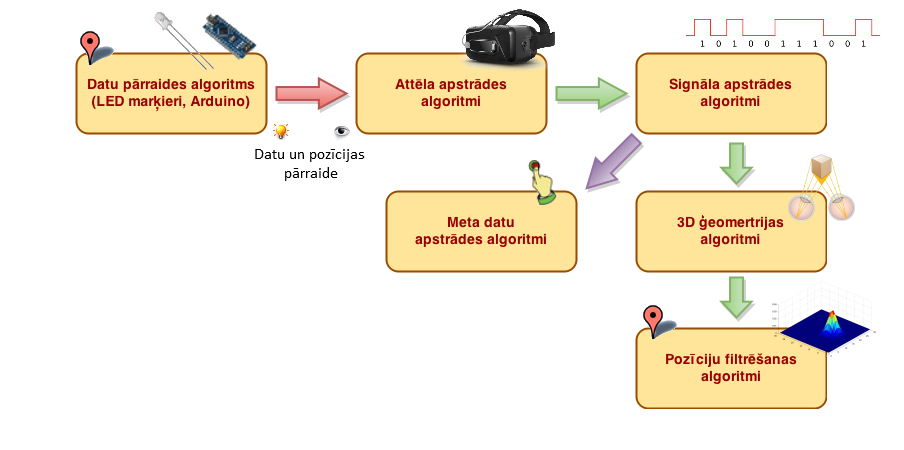
\includegraphics[width=1\columnwidth]{images/MainDiagram.png}
\begin{center}
\footnotesize{
\textit{\thecimages. attēls. Piedāvātās sistēmas darbību secību diagramma.}}
\end{center}
\end{center}
\end{samepage}


\par
Līdz šim ir veikti dažādi mēģinājumi virtuālo attēlu saistīt ar fizisko pasauli, 
lai datorsistēmas lietotājs fiziski to varētu aizskart
jeb iegūt haptisko atgriezenisko saiti. 
Nesenākā no šādām sistēmām ir MIT izstrādātā fiziski aizskaramu pikseļu virsma inFORM, 
kur katrs pikselis var tikt izbīdīts uz āru, radot reljefu un objekta apveidus 
\cite{sean_follmer_inform:_2013}. Pirms tam Walt Disney studijā izveidotā AIREAL sistēma, kas izmanto Microsoft Kinect tipa dziļuma sensoru, ir demonstrējusi skāriena imitāciju 3D telpā, izmantojot mērķētus tvaika burbuļus \cite{rajinder_sodhi_aireal:_2013}. Un vēl pirms šī pētījuma MIT laboratorijā tika izstrādāta sistēma ZeroN \cite{jinha_lee_zeron:_2011}, kas ar elektromagnētu palīdzību 3D telpā var stabili pozicionēt metāla lodīti, kuru lietotājs var izmantot saskarnei ar datoru. 
MIT pētījumā plānotā sistēma, izmantojot helikopteru, arī sasniedz līdzīgus rezultātus, bet neliela helikoptera sistēma ir daudz lētāka un vieglāk \\
adaptējama jau esošām darba vidēm. Kā arī helikoptera sistēma ir plānota darbībai tieši virtuālajā realitātē (VR), bet ZeroN, ir galvenokārt paredzēta fiziskai datora komunikācijai ar lietotāju bez atsevišķa vizuālā interfeisa. Līdzīgs risinājums ZeroN ir arī japāņu radītā 3D levitācijas metode, izmantojot skaņas viļņus \cite{yoichi_ochiai_three-dimensional_2013}, bet tā pašlaik nebūtu piemērota radīt pietiekami daudzveidīgu un precīzu taustes sajūtu virtuālās realitātes vajadzībām.
\par
Citi risinājumi atgriezeniskās saites iegūšanai izmanto speciāli izveidotus robotizētus statīvus 
vai cimdus 
\cite{jose-luis_rodrguez_haptic_2012} 
\cite{andrea_f.abate_haptic-based_2009}. 
Ir arī pētījumi, kuros analizētas iespējas radīt taustes sajūtu, 
izmantojot plašāk pieejamākas ierīces, kā, \\ piemēram, slēdžus \cite{monica_bordegoni_haptic_2006}, 
un pat veikti eksperimenti, imitējot citas formas virtuālus elementus, 
kas atšķiras no fiziski taustāmiem elementiem \cite{luv_kohli_warping_2013}. 
%
Šajā pētījumā piedāvātā sistēma virtuālajai realitātei nodrošina taustāmu atgriezenisko saiti
jebkuram fiziskam objektam, pie kura ir pievienoti infrasarkanie marķieri, kas atšķirībā no
tradicionālajiem, paplašinātajā realitātē izmantotajiem, marķieriem nav redzami cilvēka acij.
Aktīvos infrasarkanos marķierus var pievienot jebkuras formas un krāsas fiziskiem objektiem. 
Viena no \\ interesantākajām implementācijām šādai sistēmai var tik izveidota, pievienojot šādus marķierus 
fiziskā telpā kustīgiem objektiem, kuri var tikt izmantoti kā manipulatori virtuālajai realitātei, piemēram,
mazai iekštelpu helikoptera platformai, kura reprezentē taustāmas virsmas virtuālajā realitātē 
jebkurā telpas vietā.
\par
Galvenā priekšrocība infrasarkanajiem marķieriem ir tieši paplašinātajā realitātē. 
Ar tiem var iegūt precīzu objekta atrašanās vietu telpā neatkarīgi no 
šī objekta vizuālā izskata vai formas. Ar to palīdzību ir iespējams atpazīt ātri objektus, kurus
ir grūti vai neiespējami atpazīt ar tradicionālajiem redzamajiem marķieriem. Piemēram, šos
marķierus ir iespējams ievietot rotaļlietās un tām piešķirt virtuālas īpašības paplašinātajā 
vai virtuālajā realitātē.

\par
Infrasarkano marķieru pielietojumi ir daudz plašāki par virtuālo realitāti.
Tie var tikt iebūvēti ikdienā izmantojamos fiziskos objektos, piemēram, traukos,
atvieglojot robotam to atpazīšanu, tādējādi tuvinot mūs soli tuvāk robotizētai virtuvei.
Tos var izmantot arī dažādās industriālās ierīcēs, kuras var izmantot gan roboti, gan cilvēki,
piemēram, svirās un vārstuļos. Tie netraucē cilvēkam vizuāli uztvert fizisko objektu, 
bet palīdz datorsistēmai iegūt informāciju par šo objektu pozīciju un orientāciju telpā.

\par 
Vairākas neredzamu marķieru sistēmas ir izveidotas medicīnas vai ražošanas aprīkojumam \cite{WeiLiu2014} \cite{BMWServices2014}.
Šajās sistēmās tiek izmantoti statiski, bet neredzami marķieri, kas veiksmīgi kontrolētā vidē nodrošina paplašinātās
realitātes ilūziju.

%%%%%%%%%%%%%%%%%%%%%%%%%%%%%%%%%%%%%%%%%%%%%%%%%%%%%%%%%%%%%%%%%%%%%%%%%%%%%%%%%%%%%%%%%%%%%%%%%%%%%%%%%%%%%%

\newpage
\section{Risinājumi virtuālai un paplašinātai realitātei}

\par
Virtuālā un paplašinātā realitāte šajā darbā tika pētīta, izmantojot komerciālas,
visiem pieejamas, pirmās paaudzes 
%ref leap motion presentation
tehnoloģijas. Šīs iekārtas tiek sauktas par pirmās paaudzes tehnoloģijām, neskatoties
uz to, ka pirms tam tās vairākus desmitus gadu tika izmantotas akadēmiskās laboratorijās
%ref
, taču tām neizdevās piesaistīt vajadzīgo finansējumu un \\ uzņēmumus, kuri spētu tehnoloģiju
novest līdz tirgum. Pirmās paaudzes iekārtas nepiedāvā pilnu sensoro un saskarnes nodrošinājumu, 
lai būtu iespējams realizēt funkcionālu virtuālo vai paplašināto realitāti.
Šobrīd pilnu risinājumu var nodrošināt, izveidojot komplektāciju no ievades ierīcēm, sensoriem, kamerām
un pie galvas piestiprināmiem ekrāniem. \\
Sakomplektējot kameras ar virtuālās realitātes ekrāniem ir iespējams iegūt arī paplašinātās
realitātes risinājumu, jo pašlaik pieejami paplašinātās realitātes ekrāni nepiedāvā telpisku 
virtuālu objektu precīzu attēlojumu telpā.
\par
Labākās, pašlaik komerciāli pieejamās pirmās paaudzes virtuālās realitātes ekrānu iekārtas:
\begin{itemize}
\item \textbf{Oculus Rift} \hfill \\
Pie galvas piestiprināms ekrāns.\\
Ekrāna rezolūcija 1920x1080 pikseļi (960x1080 px katrai acij).\\
75 Hz frekvence attēla pārzīmēšanai.\\
100$\deg$ redzamības lauks (\textit{FOV}).\\
6 brīvības pakāpes kustībai.\\
1000 Hz žiroskops, akselometrs, magnetometrs.\\
30 Hz infrasarkanā kamera pozīcijas noteikšanai.
% atsauce uz http://doc-ok.org/?p=1124
% http://www.oculus.com

\refstepcounter{cimages}\label{cimages:OculusLeap.png.png}
\vspace{10pt}
\begin{samepage}
\begin{center}
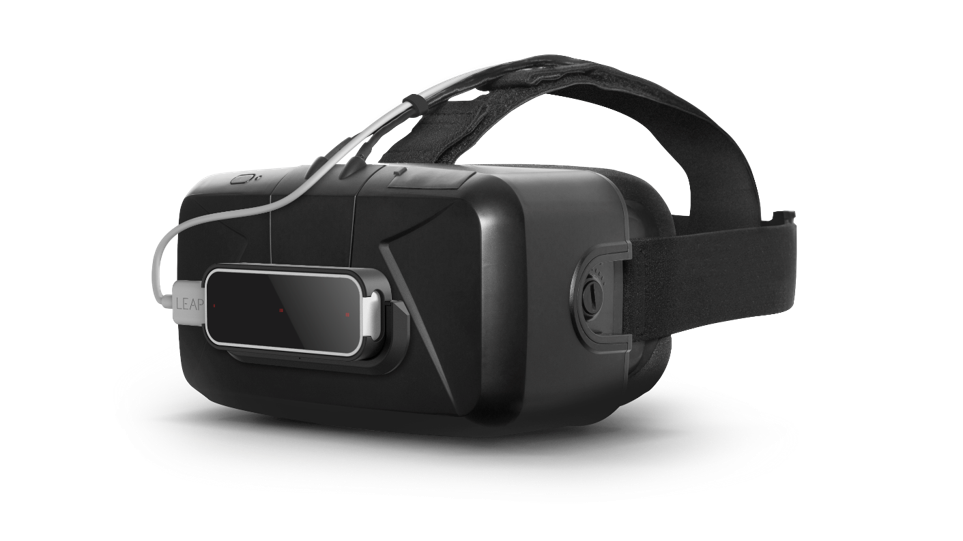
\includegraphics[width=0.8\columnwidth]{images/OculusLeap.png}
\begin{center}
\footnotesize{
\textit{\thecimages. attēls. Pētījumā izmantotais Oculus Rift DK2 ekrāns ar piestiprinātu Leap Motion sensoru.}}
\end{center}
\end{center}
\end{samepage}


\item \textbf{Sony Morpheus} \hfill \\
Pie galvas piestiprināms ekrāns.\\
Tehniskie parametri tādi paši kā Oculus Rift, 
tikai ekrāna attēla pārzīmēšanas frekvence ir 120 Hz. \\
Šobrīd, 2015. gada jūnijā nav iespējams vēl šo ierīci iegādāties.

\refstepcounter{cimages}\label{cimages:morpheus.jpg}
\vspace{10pt}
\begin{samepage}
\begin{center}
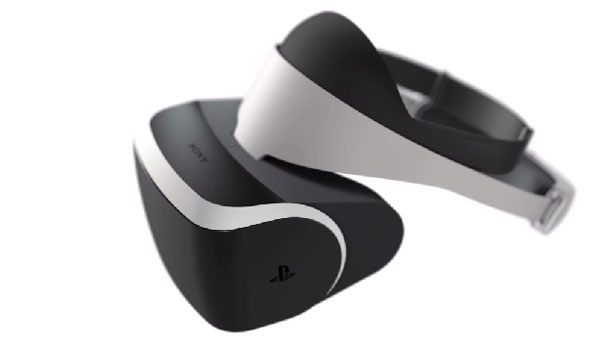
\includegraphics[width=0.4\columnwidth]{images/morpheus.jpg}
\begin{center}
\footnotesize{
\textit{\thecimages. attēls. Sony Morpheus pie galvas piestiprināms ekrāns.}}
\end{center}
\end{center}
\end{samepage}

% http://www.sony.com/SCA/company-news/press-releases/sony-computer-entertainment-america-inc/2014/sony-computer-entertainment-announces-project-morp.shtml

\item \textbf{Razer Open-Source Virtual Reality (OSVR)} \hfill \\
Pie galvas piestiprināms ekrāns.\\
Ekrāna rezolūcija 1920x1080 pikseļi (960x540 px katrai acij).\\
60 Hz frekvence attēla pārzīmēšanai.\\
100$\deg$ redzamības lauks (\textit{FOV}).\\
6 brīvības pakāpes kustībai.\\
Iekļauts žiroskops, akselometrs, magnetometrs.\\
30 Hz infrasarkanā kamera pozīcijas noteikšanai. \\
Šobrīd, 2015. gada jūnijā nav iespējams vēl šo ierīci iegādāties.

\refstepcounter{cimages}\label{cimages:osvr.jpg}
\vspace{10pt}
\begin{samepage}
\begin{center}
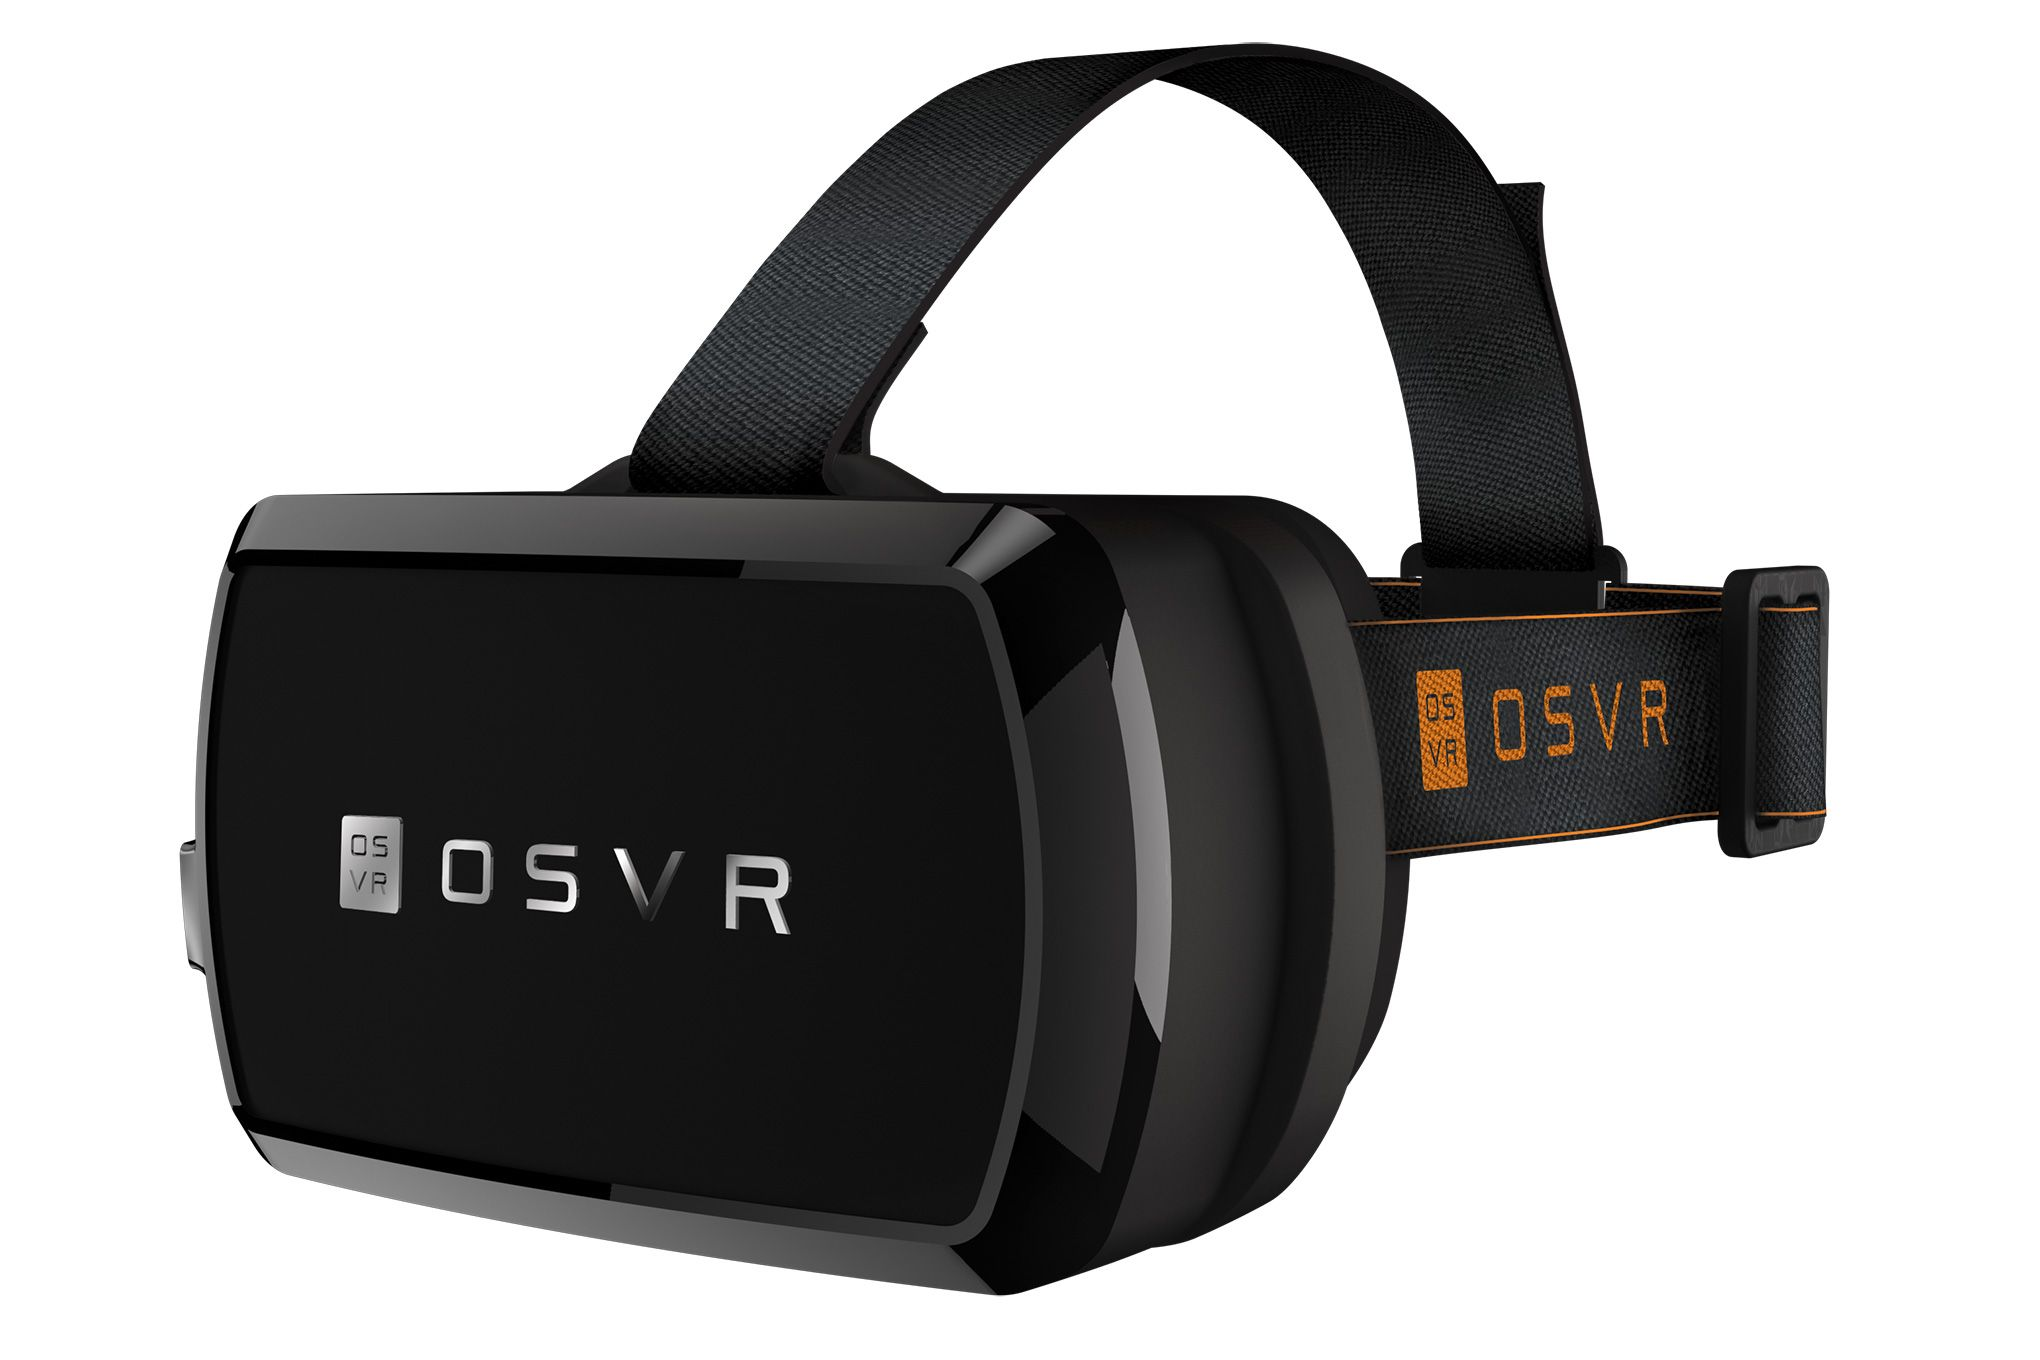
\includegraphics[width=0.4\columnwidth]{images/osvr.jpg}
\begin{center}
\footnotesize{
\textit{\thecimages. attēls. Razer OSVR pie galvas piestiprināms ekrāns.}}
\end{center}
\end{center}
\end{samepage}


\item \textbf{Samsung Gear VR} \hfill \\
Pie galvas piestiprināms ekrāna turētājs.\\
Kā ekrāns tiek izmantots viedtālrunis Samsung Galaxy Note 4.
Ekrāna rezolūcija 2560×1440 pikseļi (1280x720 px katrai acij).\\
60 Hz frekvence attēla pārzīmēšanai.\\
96$\deg$ redzamības lauks (\textit{FOV}).\\
3 brīvības pakāpes kustībai.\\
50 Hz žiroskops, akselometrs, magnetometrs.\\

Ar šo sistēmu nav iespējams precīzi noteikt kameras pārvietojumu telpā, jo
netiek izmantots ārējs atskaites marķieris, kā citās sistēmās. Priekšrocība
šai iekārtai ir tajā, ka lietotājs nav piesaistīts pie datora ar vadiem.
Lai arī mazāku dimensiju ekrāns ar augstu rezolūciju caur optiskajām lēcām 
dod labāku rezultātu kā citas iekārtas, diemžēl viedtālruņa grafiskais
procesors nevar dot pilnvērtīgu virtuālās realitātes attēlu kvalitāti.

\refstepcounter{cimages}\label{cimages:samsung_vr.jpg}
\vspace{10pt}
\begin{samepage}
\begin{center}
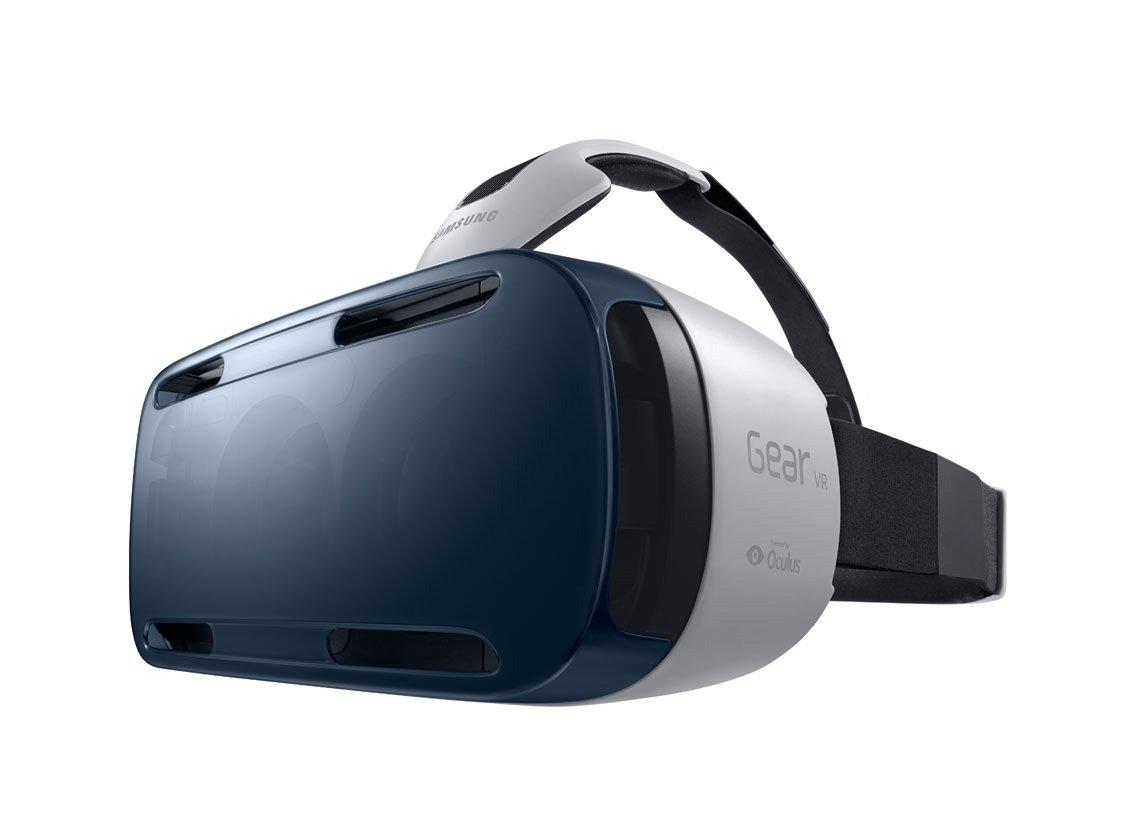
\includegraphics[width=0.4\columnwidth]{images/samsung_vr.jpg}
\begin{center}
\footnotesize{
\textit{\thecimages. attēls. Samsung Gear VR pie galvas piestiprināms ekrāna turētājs un lēcu sistēma.}}
\end{center}
\end{center}
\end{samepage}

\item \textbf{HTC SteamVR} \hfill \\
Pie galvas piestiprināms ekrāns.\\
Ekrāna rezolūcija 2160x1200 pikseļi (1080x600 px katrai acij).\\
90 Hz frekvence attēla pārzīmēšanai.\\
100$\deg$ redzamības lauks (\textit{FOV}).\\
6 brīvības pakāpes kustībai.\\
Tiek izmantoti žiroskops, akselometrs, magnetometrs, \\
un infrasarkanā kamera pozīcijas noteikšanai. \\
Šobrīd, 2015. gada jūnijā nav iespējams vēl šo ierīci iegādāties.

\refstepcounter{cimages}\label{cimages:htc.jpg}
\vspace{10pt}
\begin{samepage}
\begin{center}
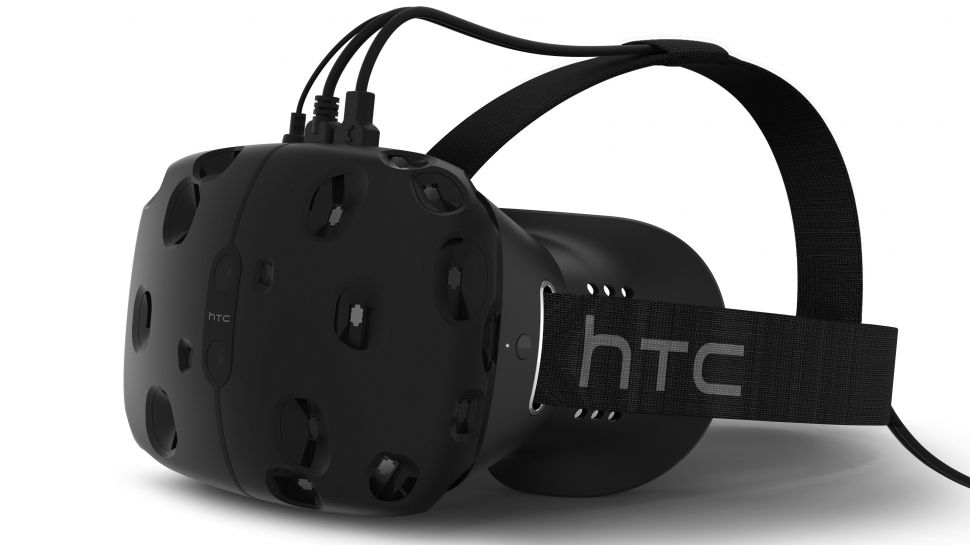
\includegraphics[width=0.4\columnwidth]{images/htc.jpg}
\begin{center}
\footnotesize{
\textit{\thecimages. attēls. HTC SteamVR pie galvas piestiprināms ekrāns.}}
\end{center}
\end{center}
\end{samepage}

\end{itemize}
\par
Pašlaik pieejamās vai izstrādē esošās pirmās paaudzes paplašinātās realitātes ekrānu iekārtas:
\begin{itemize}
\item \textbf{Meta} \hfill \\
Daļēji caurspīdīga ekrāna rezolūcija 960x540 pikseļi (480x540 px katrai acij)
23$\deg$ redzamības lauks (\textit{FOV}).\\
Aktīvs dziļuma mērīšanas sensors, izmantojot mazu infrasarkanās gaismas projektoru un 320x240 pikseļu rezolūcijas infrasarkanās gaismas kameru.
Iekārtai ir 3 brīvības pakāpes kustības noteikšanai, izmantojot žiroskopu, akselometru un magnetometru.
Tā kā iekārta līdzīgi kā Samsung Gear VR nav pievienota personālajam datoram, tad jārēķinās, ka tai nebūs pietiekamu skaitļošanas resursu
pārliecinošas paplašinātās realitātes iegūšanai. Arī šo iekārtu, šobrīd, 2015. gada jūnijā vēl nav iespējams iegādāties.
Šo ierīci ierobežoti varētu būt iespējams izmantot šajā pētījumā piedāvātajā marķieru sistēmā. 

\refstepcounter{cimages}\label{cimages:meta}
\vspace{10pt}
\begin{samepage}
\begin{center}
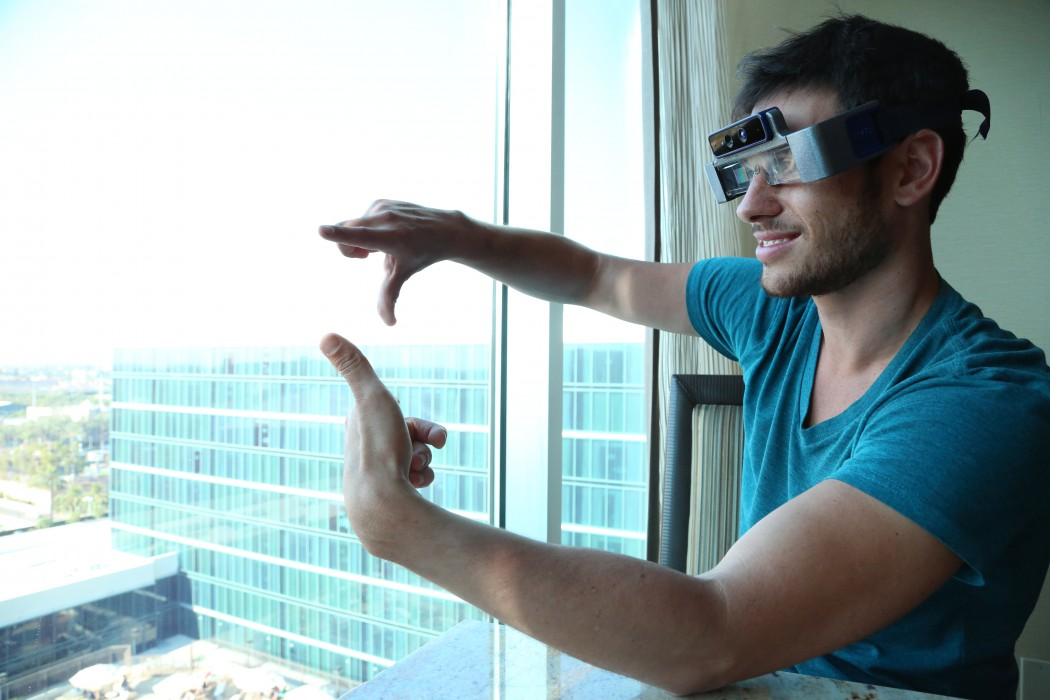
\includegraphics[width=0.4\columnwidth]{images/meta.jpg}
\begin{center}
\footnotesize{
\textit{\thecimages. attēls. Meta brilles.}}
\end{center}
\end{center}
\end{samepage}

\item \textbf{Google Glass} \hfill \\
Google Glass bija ierīce, kas tika izdota 2013. gadā un to bija iespējams iegādāties līdz 2015. gada janvārim.
Līdzīgi kā Meta brilles arī šīs cieš no tām pašām un vēl vairākām tehniskajām problēmām. 
Iekārtai ir ļoti neliels, kvadrātveida ekrāns tikai vienai acij ar 640x360 pikseļu rezolūciju.
Tāpat iekārtai nav nekādu sensoru dziļuma noteikšanai telpā, un papildinātai
realitātei nepieciešamās projekcijas nav piemērotas šādam ekrānam. 
Google Glass piedāvā paplašināto realitāti, dodot papildus grafisko informāciju par tuvumā esošiem
objektiem, neizmantojot precīzas objektu atrašanās vietas telpā. 
Vēl šīm brillēm ir pievienot liela baterija, kura uzkarst un daudziem lietotājiem sagādā galvassāpes.

\refstepcounter{cimages}\label{cimages:glass}
\vspace{10pt}
\begin{samepage}
\begin{center}
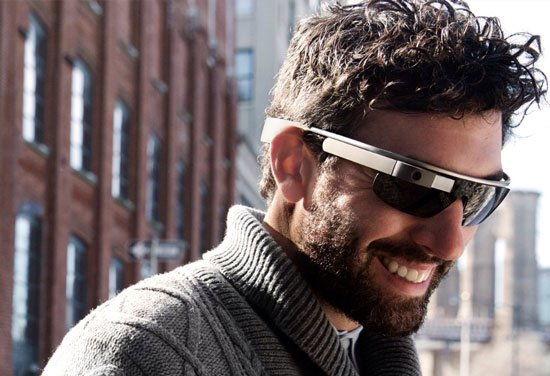
\includegraphics[width=0.4\columnwidth]{images/glass.jpg}
\begin{center}
\footnotesize{
\textit{\thecimages. attēls. Google Glass brilles.}}
\end{center}
\end{center}
\end{samepage}

\item \textbf{Microsoft Hololens} \hfill \\

Microsoft Hololens brilles vēl publiski nav iespējams iegādāties, bet ir jau pieejama ierobežota tehniskā
specifikācija, un ir iespējams novērtēt šīs ierīces piemērotību paplašinātās realitātes
marķieru sistēmām. Briļļu augšējā daļā ir ievietota Microsoft Kinect sensora tehnoloģija,
bet pašās brillēs ir neliels taisnstūra veida puscaurspīdīgs ekrāns. Ņemot vērā, ka
iekārta, tāpat kā iepriekšējās izmanto ļoti nelielu iebūvētu datoru, var prognozēt, ka
iekārtas rezultāts nedos pilnīgi saplūstošu papildinātās realitātes ilūziju, bet šī
sistēma varētu tikt pielāgota arī šajā pētījumā izmantotajai marķieru sistēmai. 
Šo iekārtu, šobrīd, 2015. gada jūnijā vēl nav iespējams iegādāties \cite{olivier_bau_revel:_2013}.

\refstepcounter{cimages}\label{cimages:holo}
\vspace{10pt}
\begin{samepage}
\begin{center}
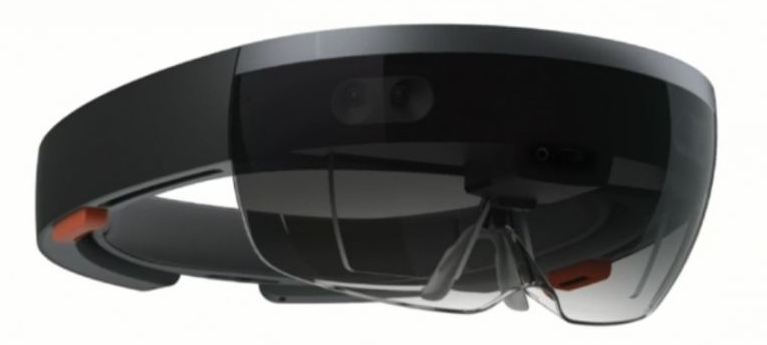
\includegraphics[width=0.4\columnwidth]{images/holo.jpg}
\begin{center}
\footnotesize{
\textit{\thecimages. attēls. Microsoft Hololens brilles.}}
\end{center}
\end{center}
\end{samepage}

\end{itemize}
\par
Labākie pašlaik pieejamie sensori un kameras virtuālās un paplašinātās realitātes sistēmām:
\begin{itemize}
\item \textbf{Leap Motion} \hfill \\
Sistēma, kas darbojas, izmantojot 2 infrasarkano staru gaismas kameras, iegūstot stereo attēlus.
Katra infrasarkanās gaismas kamera ir ar 640x240 pikseļu rezolūciju. Uz platformas ir arī
izvietotas 3 infrasarkanās gaismas diodes telpas apgaismošanai.
Iekārta paredzēta novietošanai uz galda un roku un pirkstu pozīciju un orientāciju noteikšanai,
izmantojot tikai 2 attēlus. Atšķirībā no Microsoft Kinect šī iekārta neprojicē nekādu rakstu
uz telpā esošiem objektiem. Šī pētījuma ietvaros iekārta tiek pievienota pie Oclus Rift
displeja acu augstumā. Kamera ir unikāla un īpaši piemērota šim pētījumam, jo tās
attēlu kadru frekvence ir 111 Hz. Darbības lauks šai iekārtai roku noteikšanai ir $45cm^3$.
Detalizētāks ierīces apraksts dots \ref{sensors_vr}.nodaļā.

\refstepcounter{cimages}\label{cimages:leap_example}
\vspace{10pt}
\begin{samepage}
\begin{center}
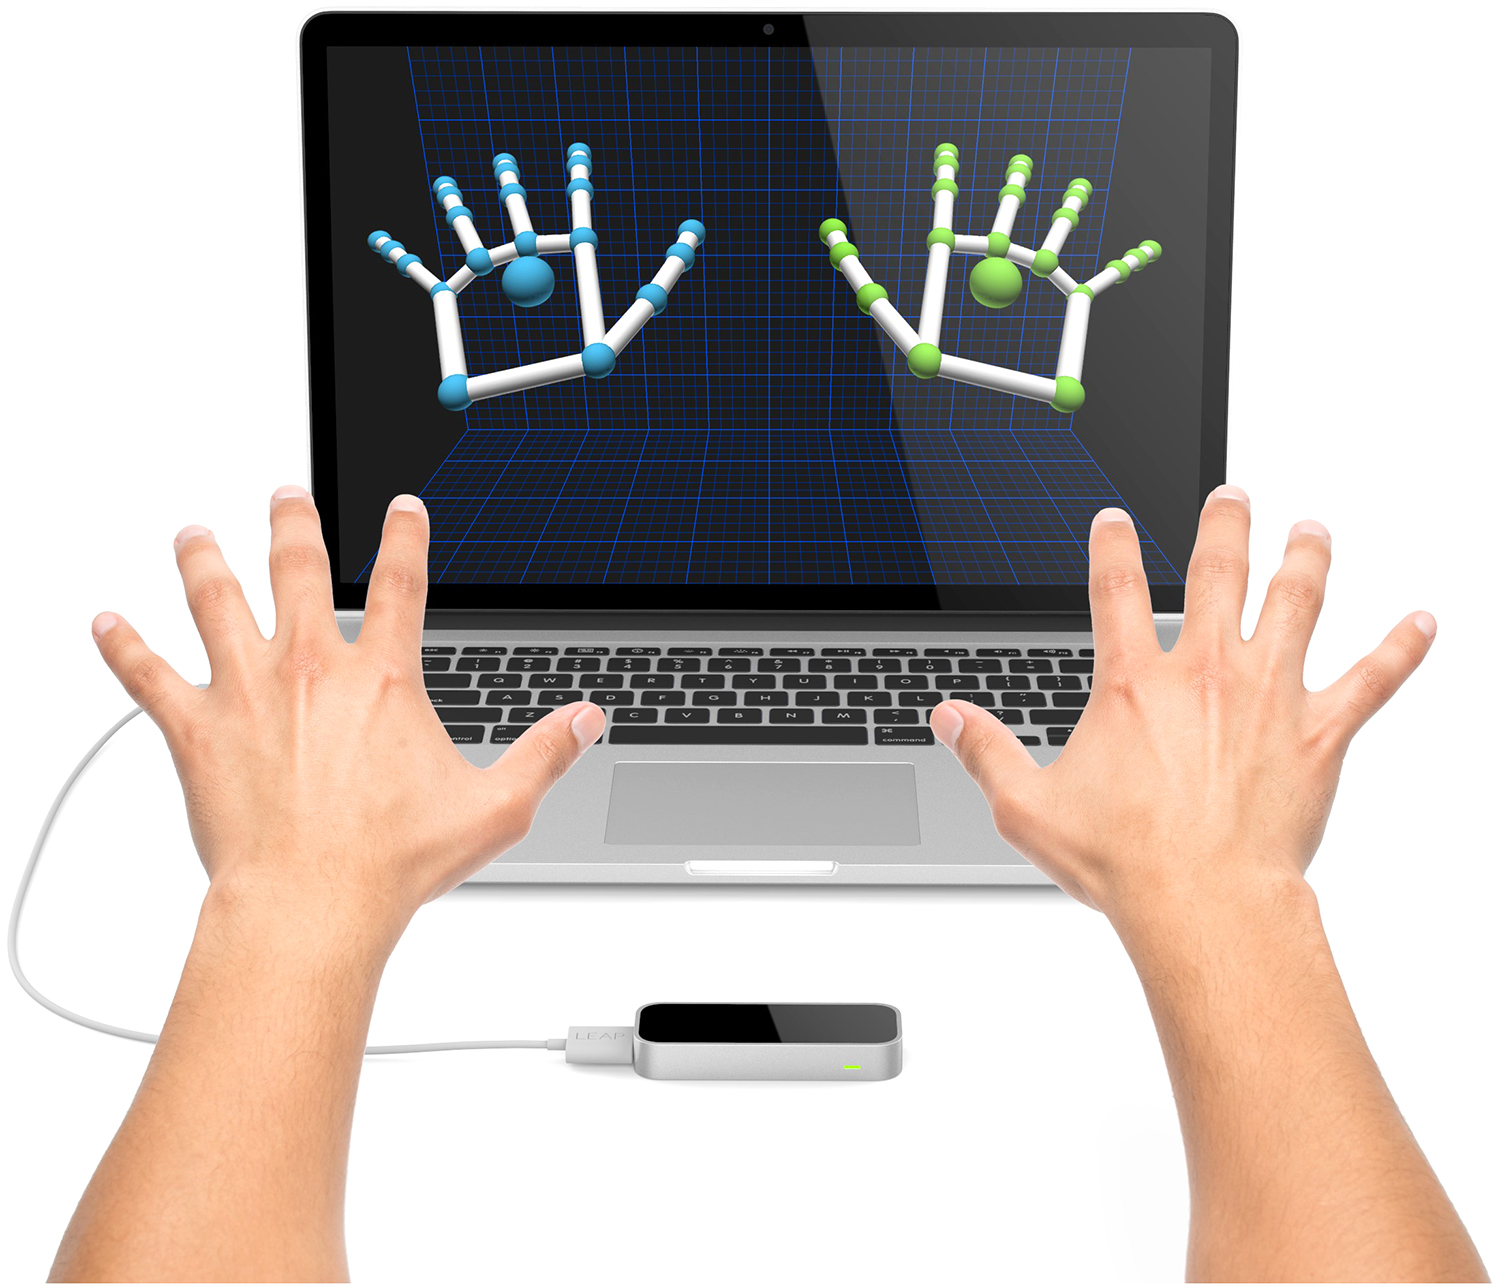
\includegraphics[width=0.5\columnwidth]{images/leap_example.jpg}
\begin{center}
\footnotesize{
\textit{\thecimages. attēls. Leap Motion stereo kamera.}}
\end{center}
\end{center}
\end{samepage}

\item \textbf{Microsoft Kinect V2} \hfill \\

\par
Microsoft piedāvātā Kinect V2 sistēma nosaka punktu dziļumu telpā, izmantojot infrasarkanās
gaismas speciāla raksta lāzera projekciju un infrasarkanās gaismas kameru.
Sensoru sistēma Microsoft Kinect V2 ir pieejama un nav piemērota šajā pētījumā piedāvātajai
marķieru sistēmai, jo tā izmanto tikai vienu kameru un speciālu lēcu sistēmu,
un no iegūtā attēla dziļuma attālumu nevar noteikt, izmantojot marķiera diodes. Tā vietā
dziļums var tikt noteikts, izmantojot tikai Kinect projekcijas rakstu. Tāpat kameras 
attēla frekvence ir pārāk maza, lai varētu veikt datu pārraidi pieņemamā ātrumā.\\

Microsoft Kinect V2 parametri:
\begin{itemize}
\item 1920 x 1080 pikseļu redzamās gaismas kamera
\item 512 x 424 pikseļu infrasarkanās gaismas kamera
\item 30 Hz kameru attēlu frekvence
\item 0.5-4.5 m darbības rādiuss
\end{itemize}

%https://msdn.microsoft.com/en-us/library/jj131033.aspx

\refstepcounter{cimages}\label{cimages:kinect2_store}
\vspace{10pt}
\begin{samepage}
\begin{center}
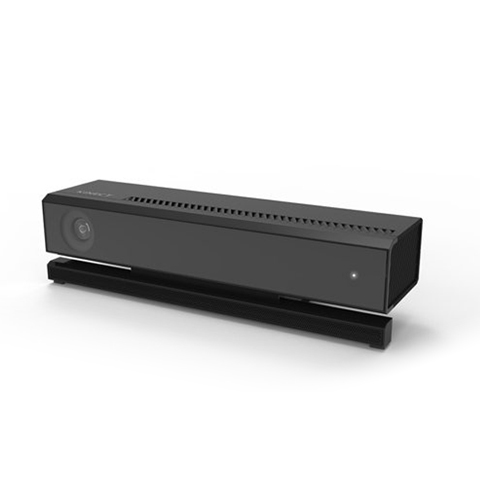
\includegraphics[width=0.4\columnwidth]{images/kinect2_store.jpg}
\begin{center}
\footnotesize{
\textit{\thecimages. attēls. Microsoft Kinect V2 sensoru sistēma.}}
\end{center}
\end{center}
\end{samepage}

\item \textbf{Creative Senz3d} \hfill \\

Creative Senz3d sensoru sistēma piedāvā tieši tās pašas funkcijas, kuras piedāvā Microsoft Kinect V2,
taču iekārta ir kompaktāka un lētāka. \\

Creative Senz3d parametri:
\begin{itemize}
\item 1280 x 720 pikseļu redzamās gaismas kamera
\item 320 x 240 pikseļu infrasarkanās gaismas kamera
\item 30 Hz kameru attēlu frekvence
\item 0.1-1.5 m darbības rādiuss
\end{itemize}

\refstepcounter{cimages}\label{cimages:creative}
\vspace{10pt}
\begin{samepage}
\begin{center}
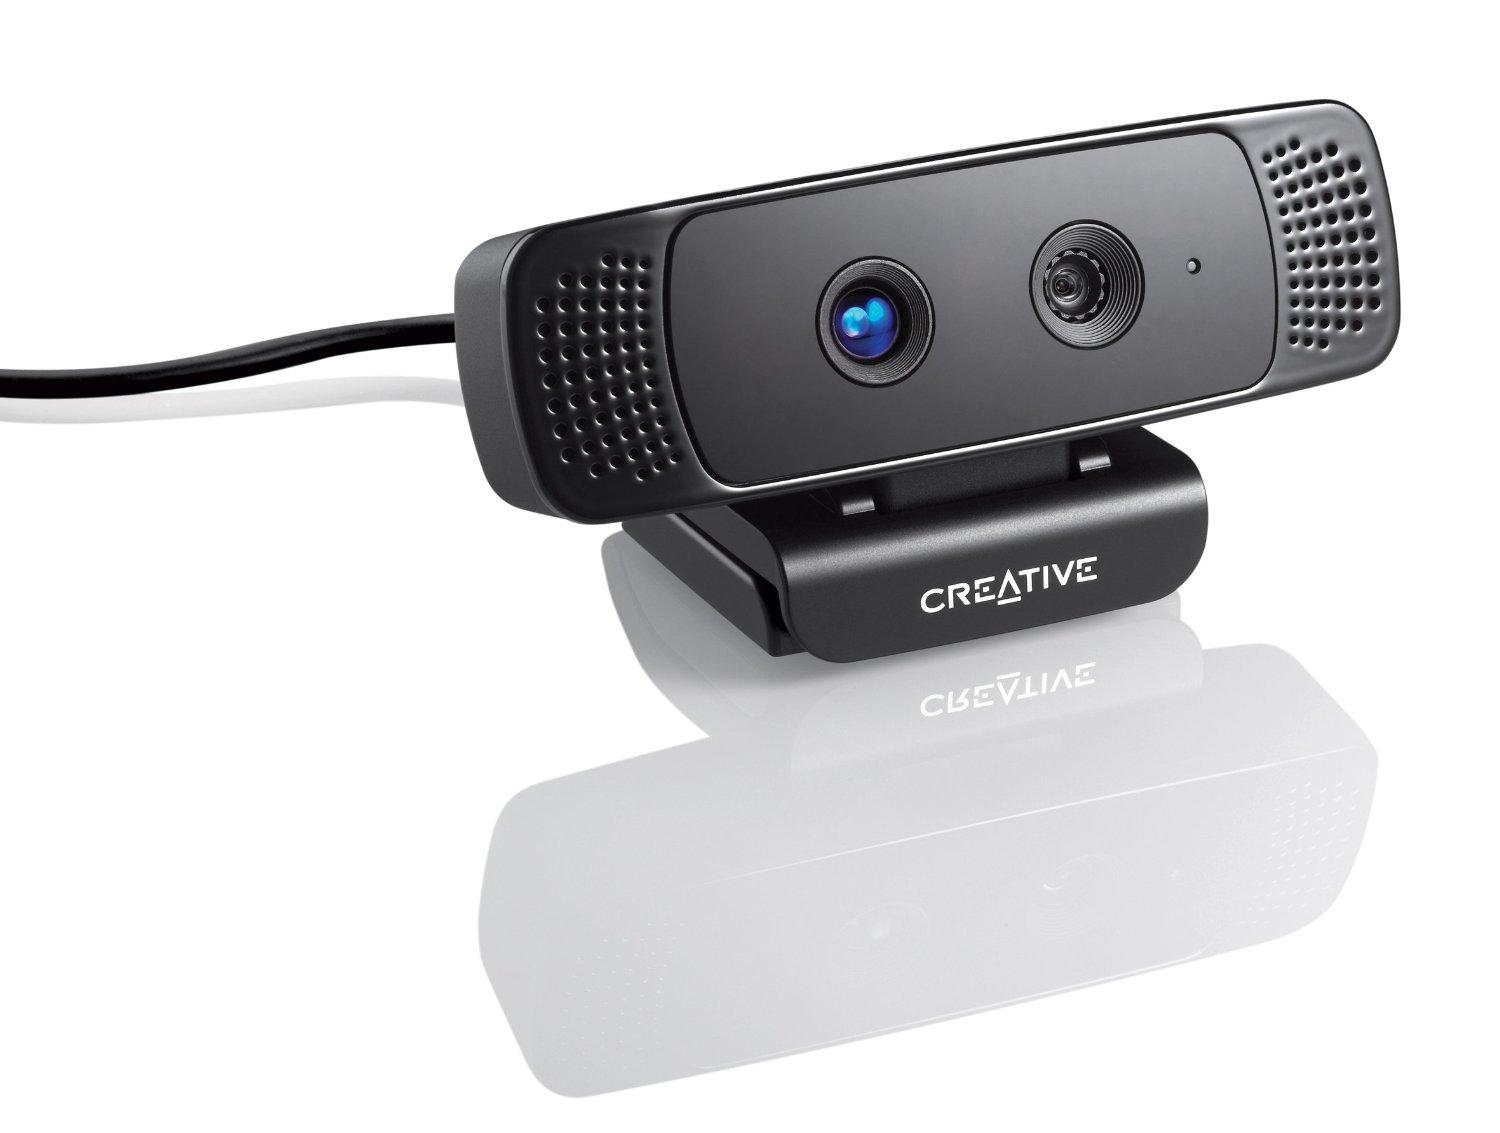
\includegraphics[width=0.4\columnwidth]{images/creative.jpg}
\begin{center}
\footnotesize{
\textit{\thecimages. attēls. Creative Senz3d sensoru sistēma.}}
\end{center}
\end{center}
\end{samepage}

\item \textbf{OVR vision} \hfill \\

OVR vision iekārta nodrošina paplašinātai realitātei nepieciešamos redzamos gaismas attēlus
katrai acij, kuri tiek projicēti uz virtuālās realitātes ekrāna. Ar šo sistēmu nevar implementēt
cilvēkam neredzamās gaismas marķieru sistēmu, bet tā būtu labs papildinājums Leap Motion sensoru
sistēmai, apslēpjot neredzamās gaismas datu pārraidi no redzamā attēla. 

OVR vision parametri:
\begin{itemize}
\item 1280 x 480 pikseļu redzamās gaismas kamera (640 x 480 pikseļi katrai acij)
\item 60 Hz kameru attēlu frekvence \cite{olivier_bau_revel:_2013}
\end{itemize}

\refstepcounter{cimages}\label{cimages:ovr}
\vspace{10pt}
\begin{samepage}
\begin{center}
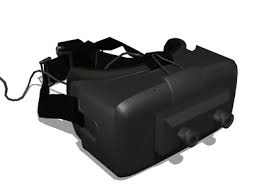
\includegraphics[width=0.4\columnwidth]{images/ovr.jpg}
\begin{center}
\footnotesize{
\textit{\thecimages. attēls. OVR vision stereo kameras sistēma, kura piestiprināta Oculus Rift DK2 iekārtas.}}
\end{center}
\end{center}
\end{samepage}

\end{itemize}
\par
Vēl bez šiem sensoriem ir pieejama virkne tradicionālu ievades iekārtu, kas piemērotas virtuālas
vai paplašinātās realitātes vajadzībām, kā piemēram, spēļu pultis, taču tās nav nepieciešamas 
sistēmas izstrādē, kas balstās uz infrasarkanās gaismas marķieriem.

\newpage
\subsection{Virtuālās un paplašinātās realitātes attēlošanas risinājumi}

\par
Virtuālai realitātei atšķirībā no 3D ekrāniem, anaglifiem, u.t.l. tehnoloģijām
jānodrošina sajūtu, izmantojot redzi, ka lietotājs fiziski atrodas virtuālā telpā.
Virtuālās realitātes ilūziju ir iespējams panākt vismaz 3 veidos:
\begin{itemize}
\item Alas sistēma (\textit{cave}), kad lietotājs atrodas speciāli
izveidotā telpā, kur uz visām sienu virsmām tiek projicēta virtuālā telpa. Šādas
sistēmas ir ārkārtīgi neparocīgas, taču daži risinājumi var tikt implementēti arī
ikdienā izmantojamās telpās, kā piemēram, Microsoft patentētā dzīvojamās istabas projekcija.
% http://mashable.com/2012/09/11/microsoft-patent-gaming-projections/
% http://appft1.uspto.gov/netacgi/nph-Parser?Sect1=PTO2&Sect2=HITOFF&p=1&u=%2Fnetahtml%2FPTO%2Fsearch-bool.html&r=1&f=G&l=50&co1=AND&d=PG01&s1=20120223885.PGNR.&OS=DN/20120223885RS=DN/20120223885

\refstepcounter{cimages}\label{cimages:cave}
\vspace{10pt}
\begin{samepage}
\begin{center}
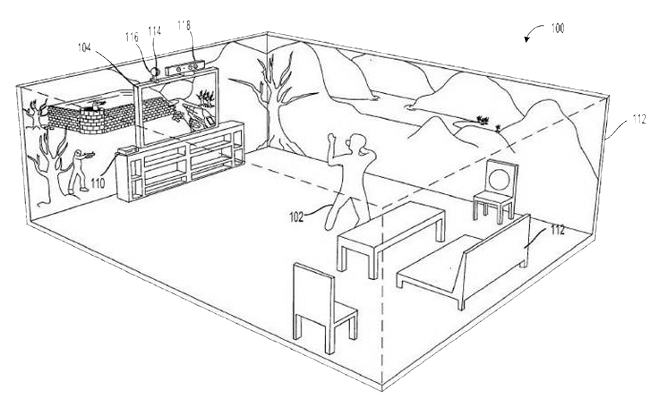
\includegraphics[width=0.6\columnwidth]{images/cave.jpg}
\begin{center}
\footnotesize{
\textit{\thecimages. attēls. Microsoft izveidotā alas veida virtuālās realitātes projekcija (ASV patents nr.20120223885).}}
\end{center}
\end{center}
\end{samepage}



\item Pie galvas piestiprināts ekrāns (\textit{HMD}) ar lēcām. Katrai acij tiek projicēts savs
attēls, kurš mainās atbilstoši galvas orientācijai un pārvietojumam, izmantojot papildus sensorus.
Šī veida ekrāni tika izmantoti šajā pētījumā.
%TODO stereo vision info


\item Pie galvas piestiprināti projektori, kuri projicē attēlu tieši acs tīklenē. Priekšrocība 
šādam risinājumam ir tā, ka šī iekārta neaizsedz visu lietotāja redzamības lauku. Šobrīd
pie šādas tehnoloģijas strādā Google uzņēmums Magic Leap \cite{SebastianAnthony2014} \cite{PaulRidden2013}.
% http://www.magicleap.com/#/home
% http://www.extremetech.com/extreme/191909-google-joins-the-vr-war-invests-in-light-field-cinematic-reality-company-magic-leap

% http://www.ife.ee.ethz.ch/education/sada/winter03_vrd3
% http://www.gizmag.com/avegant-glyph/30233/

\refstepcounter{cimages}\label{cimages:retina_display}
\vspace{10pt}
\begin{samepage}
\begin{center}
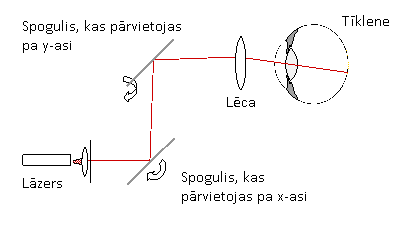
\includegraphics[width=0.6\columnwidth]{images/retina_display.png}
\begin{center}
\footnotesize{
\textit{\thecimages. attēls. Tīklenes projekcijas sistēma VRD (\textit{Virtual Retina Display}).}}
\end{center}
\end{center}
\end{samepage}


\end{itemize}
\par
Pētījuma ietvaros tika notestēta Oculus Rift pirmā versija DK1 (2013.g.), kurai bija
virkne nepilnību, kuru dēļ to nebija iespējams pilnvērtīgi lietot iecerētās sistēmas realizācijai.
Galvenā problēma DK1 ir odometrijas kļūdu akumulācija, kas rodas, aprēķinot pārvietojumu galvai, 
izmantojot tikai akselometru. 
\par
Lai to atrisinātu, Oculus Rift otrā versija DK2 (2014.g.) izmanto ārēju, stacionāru, 
infrasarkano kameru un infrasarkanos marķierus, kuri izvietoti zem ekrāna korpusa, 
kas piestiprināts pie galvas. Ar šādas sistēmas palīdzību ir iespējams iegūt precīzu relatīvu
atrašanās vietu un orientāciju, kas ir svarīga, lai varētu strādāt ar fiziskiem marķieriem telpā.
Tieši Oculus Rift DK2 tika izmantota kā platforma piedāvātās sistēmas izveidē.
\par
Pētījuma ietvaros netika izmantotas paplašinātās realitātes ekrānu iekārtas, jo to funkcionalitāte
pagaidām neļauj realizēt fizisku marķieru sasaisti ar virtuālo telpu precīzās pozīcijās un orientācijas.
\par
Pat potenciāli labākais tirgū pieejamais risinājums, META brilles, piedāvā niecīgu attēla rezolūciju 480x540 px (vienai acij),
salīdzinājumā ar Oculus Rift DK2 \\ 960x1080 px. 

\newpage
\subsection{Sensori virtuālai realitātei}\label{sensors_vr}

% infrared camera connection oculus cable
\par
Virtuālās realitātes ilūzijas iegūšanai ārkārtīgi svarīgi ir iegūt precīzu galvas pozīciju un
orientāciju, kuru nodrošina sensori, kas parasti ir izvietoti pie galvas piestiprinātajā ekrānā.
Oculus Rift gadījumā orientācija tiek noteikta, izmantojot žiroskopu un \\ magnetometru, 
savukārt pārvietojumu nosaka akselometrs un stacionāri novietota infrasarkanās gaismas kamera.

\refstepcounter{cimages}\label{cimages:TrackingCameraGood}
\vspace{10pt}
\begin{samepage}
\begin{center}
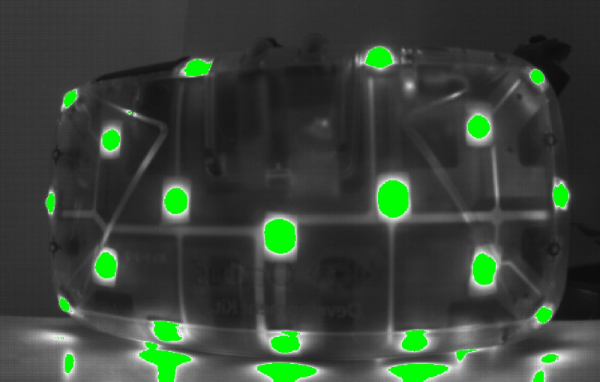
\includegraphics[width=0.5\columnwidth]{images/a6.png}
\begin{center}
\footnotesize{
\textit{\thecimages. attēls. Infrasarkanās gaismas diodes zem Oclus Rift korpusa, kuras paredzētas iekārtas pozīcijas noteikšanai. 
Lai sinhronizētu diožu darbību ar kameras kadru laiku, tiek izmantots papildus vads starp šīm divām ierīcēm.}}
\end{center}
\end{center}
\end{samepage}

\par
Lai nodrošinātu cilvēka roku un pirkstu pozīciju noteikšanu telpā, kuru var izmantot, lai to pēc tam 
rekonstruētu un attēlotu virtuālajā telpā, var izmantot virkni dažādu sensoru, kā iepriekš pieminētos PrimeSense, Kinect V2
vai Leap Motion. Leap Motion sensoram nav publiski pieejamas informācija par tajā izmantoto tehnoloģiju no tā ražotāja, taču
to ir detalizēti izpētījuši slovēņu zinātnieki \cite{JozeGuna2014}. Tā darbības attālums ir no 2.5 cm līdz 60 cm, lai
veiktu roku un pirkstu pozīciju atpazīšanu. Tas darbojas, izmantojot divas infrasarkano staru kameras ar 850nm filtru.
Pētījumā tika noskaidrots, ka Leap Motion sensora precizitāte ir ar nobīdi zem 0.5 mm. Mērījumu veikšana bija apgrūtināta
arī dēļ nestabilas kameru attēlu filmēšanas frekvences, kas ietekmē arī šajā darbā piedāvātās infrasarkano marķieru sistēmas
darbību. Pētot publiski pieejamo informāciju no Leap Motion patentu dokumentiem (US2013/0182079, US2013/0182897, US2013/0182902), 
var secināt, ka iegūtie attēli neveido punktu mākoni, bet gan meklē pozīcijas tikai objektiem, kuri atgādina rokas vai pirkstus.
Neskatoties uz to, ka no šī sensora nav iespējams iegūt punktu mākoni telpā, tas dod iespēju iegūt augstas frekvences (111Hz)
infrasarkano attēlu, kuru var izmantot pēcapstrādē, lai iegūtu informāciju par infrasarkanajiem marķieriem telpā.

\refstepcounter{cimages}\label{cimages:JozeGuna2014}
\vspace{10pt}
\begin{samepage}
\begin{center}
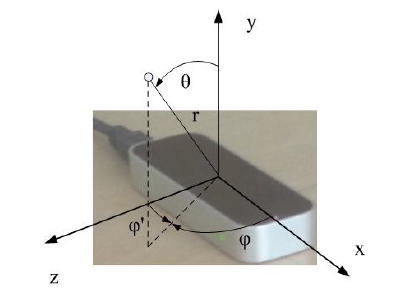
\includegraphics[width=0.5\columnwidth]{images/JozeGuna2014.png}
\begin{center}
\footnotesize{
\textit{\thecimages. attēls. Leap Motion sensors ar tajā izmantoto koordinātu sistēmu.}}
\end{center}
\end{center}
\end{samepage}

\par
Lai nodrošinātu pilnvērtīgu saskarni ar virtuālo realitāti, pie Oculus Rift var piestiprināt papildus
sensorus vai kameras, lai uztvertu roku pozīcijas un apkārtējo vidi. Šajā darbā tika izmantots Leap Motion
sensors, kas izmanto 2 infrasarkanās gaismas kameras, kuras darbojas ar 111Hz frekvenci. 
No iegūtajiem attēliem Leap Motion izrēķina roku pozīcijas pēc patentētiem algoritmiem.
%ref patens leap motion
Pētījumā šie attēli tika izmantoti, lai nolasītu infrasarkano staru marķieru pārraidītos datus,
pēc kuriem, izmantojot ģeometrisku aprēķinu no stereo kamerām, tika aprēķinātas marķieru pozīcijas telpā
pret kameru. 
Tādu pašu implementāciju infrasarkaniem marķieriem var realizēt arī bez stereo kameras, piemēram,
izmantojot Kinect V2 sensoru, kam ir tikai viena infrasarkanā kamera (30 Hz). Šajā gadījumā
marķieru pozīciju var aprēķināt ar tuvinājumu vienādojumu sistēmas risināšanā (PnP problēma).
Risinājumus var iegūt ar Levenberg-Marquardt optimizācijas algoritmu, X.S. Gao, X.-R. Hou, J. Tang, H.-F. Chang "perspektīvas trīs punktu" algoritmu
vai \\ F.Moreno-Noguer, V.Lepetit and P.Fua metodi kameras pozīcijas noteikšanai.

%TODO Solve PnP
% Iterative method is based on Levenberg-Marquardt optimization. In this case the function finds such a pose that minimizes reprojection error, that is the sum of squared distances between the observed projections imagePoints and the projected (using projectPoints() ) objectPoints .
% Method is based on the paper of X.S. Gao, X.-R. Hou, J. Tang, H.-F. Chang “Complete Solution Classification for the Perspective-Three-Point Problem”. In this case the function requires exactly four object and image points.
% Method has been introduced by F.Moreno-Noguer, V.Lepetit and P.Fua in the paper “EPnP: Efficient Perspective-n-Point Camera Pose Estimation

\newpage
\subsection{Sensori paplašinātai realitātei}

\par
Sensori, kas izmantojami virtuālai realitātei, ir piemēroti arī paplašinātās realitātes \\
nodrošināšanai. Taču praktiskai pielietojamībai nosacījums šiem sensoriem ir tāds, ka tie var tikt ērti piestiprināmi pie
paša lietotāja, lai to izmantojamība netiktu ierobežota stacionārā sistēmas konfigurācijā,
kas nav problēma virtuālās realitātes gadījumā. 

\par
Sensori paplašinātās realitātes nodrošināšanai neaprobežojas tikai ar kamerām, bet var tikt izmantotas 
arī analogas gaismas diodes. Šādas diodes izmanto televīzijas tālvadības pultīs. Ja tās novietot iepriekš
zināmā ģeometriskā konfigurācijā, tad no iegūtajiem datiem ir iespējams rekonstruēt pārraidošās gaismas
diodes atrašanās vietu. Ar šādu sistēmu, izmantojot diodes, kuras izvietotas uz ģeometriskas kuba struktūras (\prettyref{cimages:ThibautRaharijaona2013_1} attēls), 
veiksmīgi var tikt atrastas objektu pozīcijas reālā laikā, kā to ir demonstrējuši franču zinātnieki \cite{ThibautRaharijaona2013}.

\refstepcounter{cimages}\label{cimages:ThibautRaharijaona2013_1}
\vspace{10pt}
\begin{samepage}
\begin{center}
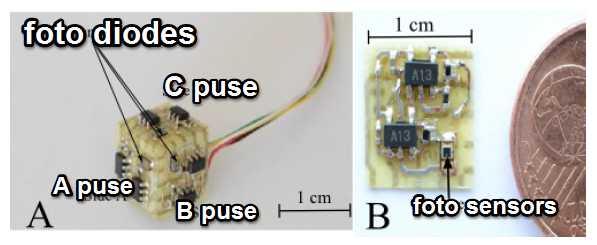
\includegraphics[width=0.5\columnwidth]{images/ThibautRaharijaona2013_1.png}
\begin{center}
\footnotesize{
\textit{\thecimages. attēls. Infrasarkano diožu konfigurācija kuba formā, lai noteiktu pārraidītāja diodes pozīciju telpā.}}
\end{center}
\end{center}
\end{samepage}

\newpage
\subsection{Redzamie marķieri paplašinātajai realitātei}

\par
Pēdējos gados redzamo marķieru tehnoloģija ir strauji attīstījusies no melnbaltiem \\ kvadrātveida simboliem
līdz jebkuras noteiktas formas plakanam attēlam vai virsmai. 

\refstepcounter{cimages}\label{cimages:a2}
\vspace{10pt}
\begin{samepage}
\begin{center}
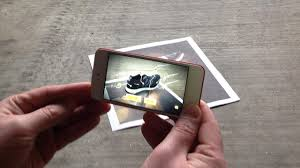
\includegraphics[width=0.5\columnwidth]{images/a2.jpg}
\begin{center}
\footnotesize{
\textit{\thecimages. attēls. Taisnstūra attēls, kas tiek izmantots kā marķieris paplašinātajai realitātei.}}
\end{center}
\end{center}
\end{samepage}

Neskatoties uz to, šo marķieru funkcionalitāte nereti apgrūtina lietotāju, jo cilvēkam pielietojamu
objektu virsmas ne vienmēr ir piemērotas marķieru izvietošanai, kā arī tas nav praktiski telpiskam objektam visas 
šķautnes apdrukāt ar redzamiem marķieriem.

\par
Vēl bieži tiek izmantotas redzamas retroflektīvu jeb atstarojošu marķieru konfigurācijas. Nereti
tā sastāv no nelielu, atstarojošu bumbiņu ģeometriskas konfigurācijas, kuru pozīcijas filmē ar vienu vai 
vairākām kamerām. Šie atstarojošie elementi var atstarot gaismu infrasarkanajā spektrā un pie kamerām 
var izvietot infrasarkano apgaismojumu. Izmantojot infrasarkano gaismas spektru un kameras filtrus, 
var mazināt kļūdu varbūtību, identificējot marķierus kameras attēlos. Šādas sistēmas ir pat uzstādītas
uz kvadrokopteriem, lai nodrošinātu savstarpēju pozīciju koordināciju \cite{MarkCutler2013}. Dotajā piemērā
tika izmantota 100Hz infrasarkanā kamera un 3 marķieru konfigurācija. 
Problēma ar šādām vienkāršām marķieru sistēmām ir tā, ka visi marķieri izskatās vienādi no kameras iegūtajā attēlā,
un, lai tos identificētu, tiek izmantotas ļoti ierobežotas ģeometriskas metodes. Piemēram, marķieru
secīgs attālums no kameras attēla augšējās daļas. Taču šāda metode nepareizi identificēs marķierus,
ja kamera tiks pagriezta lielā leņķī vai tā būs novietota uz sāniem. Tāpat šāda sistēma nav piemērota, lai 
to piestiprinātu ikdienā izmantojamiem priekšmetiem, kā arī tās darbība ir apgrūtināta, ja telpā atrodas
vairākas šādas marķieru konfigurācijas vienlaicīgi.

\refstepcounter{cimages}\label{cimages:MarkCutler2013_1}
\vspace{10pt}
\begin{samepage}
\begin{center}
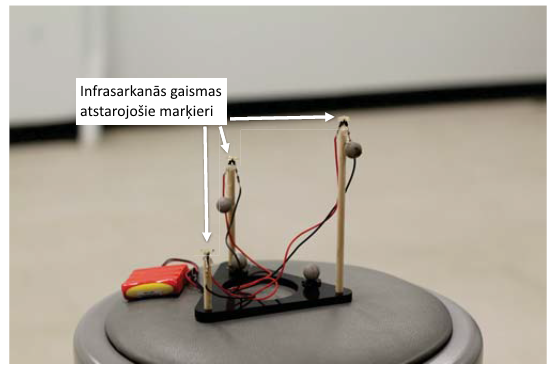
\includegraphics[width=0.5\columnwidth]{images/MarkCutler2013_1.png}
\begin{center}
\footnotesize{
\textit{\thecimages. attēls. Infrasarkano marķieru sistēma, izmantojot atstarojošos elementus.}}
\end{center}
\end{center}
\end{samepage}

\refstepcounter{cimages}\label{cimages:MarkCutler2013_2}
\vspace{10pt}
\begin{samepage}
\begin{center}
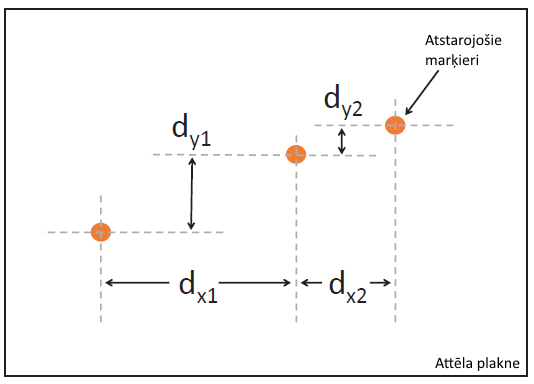
\includegraphics[width=0.5\columnwidth]{images/MarkCutler2013_2.png}
\begin{center}
\footnotesize{
\textit{\thecimages. attēls. Statisku marķieru pozīcijas attēla plaknē. Marķieri tiek identificēti pēc to attāluma no attēla plaknes augšējās daļas.}}
\end{center}
\end{center}
\end{samepage}

\refstepcounter{cimages}\label{cimages:MarkCutler2013_13}
\vspace{10pt}
\begin{samepage}
\begin{center}
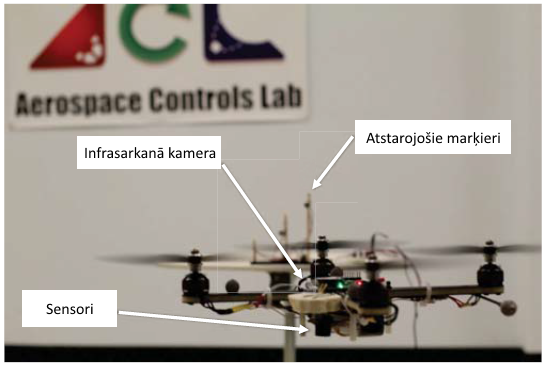
\includegraphics[width=0.5\columnwidth]{images/MarkCutler2013_3.png}
\begin{center}
\footnotesize{
\textit{\thecimages. attēls. Statisko infrasarkano marķieru sistēma, kas izvietota uz lidojošas kvadrokoptera platformas.}}
\end{center}
\end{center}
\end{samepage}

\par
%PnPSolve


\par
Šajā darbā piedāvātā infrasarkanās gaismas komunikācija nav saistīta ar Li-Fi, kas ir augstas
frekvences datu pārraide, izmantojot redzamo vai neredzamo gaismu. Piedāvātajā sistēmā kā datu
saņēmējs tiek izmantota infrasarkanā kamera, ar kuras palīdzību tiek aprēķināta gaismas avota
relatīvā pozīcija telpā attiecībā pret kameru. Savukārt Li-Fi un citos datu pārraides risinājumos,
izmantojot gaismu, pārsvarā kā datu uztvērējs tiek lietota fotodiode \cite{StefanSchmid2013} \cite{JosefZiegler2014} \cite{StefanMangold2013}. 
Izmantojot LeapMotion
kameru, marķieru datu lasīšanas funkcija papildina šīs kameras pamatfunkciju, kas ir roku un pirkstu
pozīciju noteikšana un attēla iegūšana paplašinātās realitātes iegūšanai no stereo kamerām, kuras
piestiprinātas pie Oculus Rift. Datu pārraide, izmantojot redzamās gaismas marķierus un kameru,
ir implementēta Casio PicapiCamera, MIT NewsFlash un PureVLC produktos. Šīs sistēmas piedāvā ļoti
lēnu datu pārraidi, kuru ierobežo telefona kameras kadru frekvence, \\ apgaismojums un skaitļošanas
resursi. Piemēram ar Casio PicapiCamera 8 bitu datu virknes ir jāpārraida vairākas sekundes.

\refstepcounter{cimages}\label{cimages:CasioPicapiCamera}
\vspace{10pt}
\begin{samepage}
\begin{center}
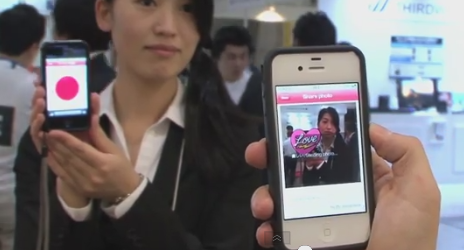
\includegraphics[width=0.5\columnwidth]{images/CasioPicapiCamera.png}
\begin{center}
\footnotesize{
\textit{\thecimages. attēls. Redzamās gaismas datu pārraide, izmantojot Casio PicapiCamera programmatūru.}}
\end{center}
\end{center}
\end{samepage}

\par
Alternatīvs risinājums visām redzamām marķieru sistēmām ir par marķieriem izmantot jau
telpā vai objektā esošās iezīmes \cite{MasayukiKanbara2002} \cite{GeorgKlein2007}. 
Iegūtie rezultāti, izmantojot pašlokalizācijas algoritmus, kā EKF-SLAM u.c \cite{MontemerloThrunKollarWegbreit} \cite{SebastianThrun}. nodrošina
augstu precizitāti, bet ir problemātiski interpretēt atrastos objektus, lai pie tiem pievienotu
informāciju paplašinātajā realitātē. Šāda sistēma ir arī jūtīga pret objektu izkārtojuma izmaiņām
telpā.

\refstepcounter{cimages}\label{cimages:a3}
\vspace{10pt}
\begin{samepage}
\begin{center}
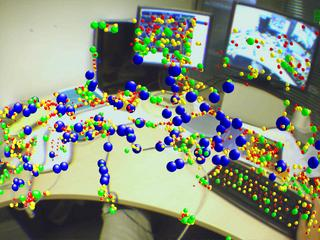
\includegraphics[width=0.5\columnwidth]{images/a3.png}
\begin{center}
\footnotesize{
\textit{\thecimages. attēls. Marķieru sistēma, izmantojot apkārtējo objektu iezīmes un EKF-SLAM algoritmu.}}
\end{center}
\end{center}
\end{samepage}

\newpage
\subsection{Neredzamie marķieri paplašinātajai realitātei}

\par
Neredzamo marķieru sistēmas pārsvarā līdz šim ir tikušas izmantotas kinematogrāfijā, ierakstot
aktieru kustības, sejas izteiksmes u.t.t. Nereti tiek izmantoti retroreflektīvie infrasarkanie
marķieri, kuri izveidoti no spoguļveidīga materiāla, kurš atstaro gaismu infrasarkanajā gaismas spektrā. 
Šī marķieru sistēma darbojas, izmantojot infrasarkano kameru ar attēlu iegūšanas frekvenci līdz pat 1000 Hz.
Salīdzinājumā infrasarkanā kamera, kas tika izmantota šajā pētījumā, spēj iegūt attēlus ar 111 Hz frekvenci, bet,
piemēram, Microsoft Kinect kamera spēj iegūt infrasarkanos attēlus tikai ar 30 Hz frekvenci. 
Jo lielāka attēlu iegūšanas frekvence, jo precīzāk ir iespējams izsekot marķiera pārvietojumu attiecībā pret
kameru, novēršot vajadzību identificēt katru marķieri pēc katra tā \\ pārvietojuma.
Kinematogrāfijā aktīvās infrasarkano marķieru sistēmas identificē marķierus, tikai uzsākot scēnas filmēšanu,
bet pēc tam izseko tikai to pārvietojumam. Parasti kinematogrāfijā tiek lietotas pasīvas infrasarkano marķieru sistēmas,
kur mākslinieks pēc filmēšanas manuāli atzīmē katra marķiera atsauces 3D modelēšanas programmatūrā.
\par 
Viena no aktīvo infrasarkano marķieru priekšrocībām atšķirībā no visām citām \\ datorredzē izmantotajām 
marķieru sistēmām ir tā, ka tos ir iespējams paslēpt zem \\ infrasarkano gaismu neabsorbējošiem materiāliem,
piemēram, dažādu veidu plastmasas. Paslēpjot diodes zem objekta korpusa vai tā virsmas, tās būs
redzamas infrasarkanās gaismas kamerai, bet ne cilvēka acij vai redzamās gaismas kamerai.
Šādā veidā, novietojot diodes zem sarežģīta telpiska objekta virsmas, ir iespējams noteikt šī objekta
pozīciju un orientāciju telpā, nemainot tā izskatu redzamajā gaismas spektrā.

%TODO info par materiāliem, kas laiž cauri IR

\par
Infrasarkano diožu pozīciju noteikšana telpā ir arī veiksmīgi tikusi realizēta, izmantojot diodes ar dažādām
mirgošanas frekvencēm (11.5 kHz, 3.5 kHz, 1kHz) un ar analogām uztveršanas diožu shēmām (\prettyref{cimages:ThibautRaharijaona2013_2}., \prettyref{cimages:ThibautRaharijaona2013_3} attēli). 
Ar šādu sistēmu franču zinātniekiem ir
izdevies veiksmīgi vadīt kvadrokopterus reāla laikā \cite{ThibautRaharijaona2013}. Šādas sistēmas 
priekšrocība ir implementācijas vienkāršībā, taču šāda sistēma nav pielietojama, ja telpā var atrasties
dažādi objekti ar dažādiem infrasarkanās gaismas datu pārraides protokoliem, kuri arī izmanto infrasarkanos marķierus pozīciju noteikšanai.

\refstepcounter{cimages}\label{cimages:ThibautRaharijaona2013_2}
\vspace{10pt}
\begin{samepage}
\begin{center}
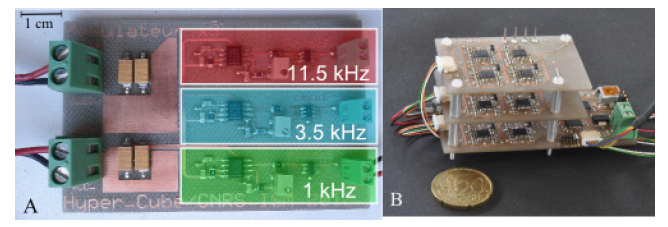
\includegraphics[width=0.5\columnwidth]{images/ThibautRaharijaona2013_2.png}
\begin{center}
\footnotesize{
\textit{\thecimages. attēls. Infrasarkano diožu konfigurācija kvadrokoptera pozīcijas noteikšanai.}}
\end{center}
\end{center}
\end{samepage}

\refstepcounter{cimages}\label{cimages:ThibautRaharijaona2013_3}
\vspace{10pt}
\begin{samepage}
\begin{center}
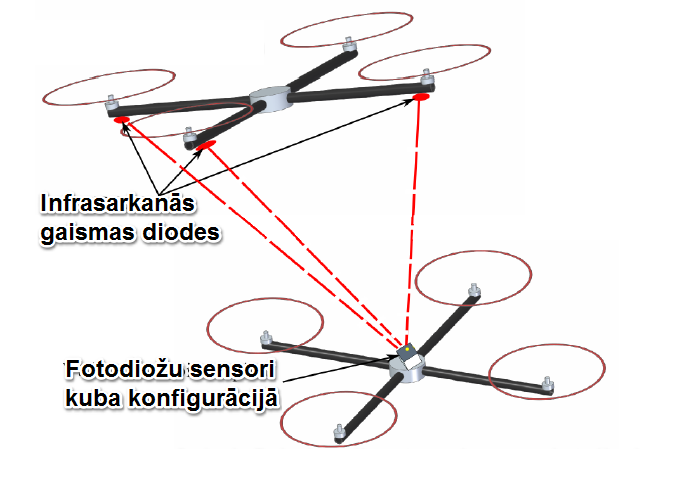
\includegraphics[width=0.5\columnwidth]{images/ThibautRaharijaona2013_3.png}
\begin{center}
\footnotesize{
\textit{\thecimages. attēls. Kvadrokopteru sistēma balstoties uz 3 aktīviem infrasarkanajiem marķieriem.}}
\end{center}
\end{center}
\end{samepage}

\par
Cilvēkam neredzamus marķierus objektu pozīcijai un orientācijai telpā var nodrošināt, izmantojot 
infrasarkanās gaismas projektoru. Šis projektors var attēlot tradicionālos kvadrātveida marķierus, kuri
ir redzami tikai infrasarkanās gaismas kamerām (\prettyref{cimages:WeiChan2010_1} attēls). 
Japāņu zinātnieku piedāvātajā risinājumā šis projektors
var attēlot arī redzamās gaismas projekcijas, tā paplašinot attēla funkcionalitāti\cite{Li-WeiChan2010}.

\refstepcounter{cimages}\label{cimages:WeiChan2010_1}
\vspace{10pt}
\begin{samepage}
\begin{center}
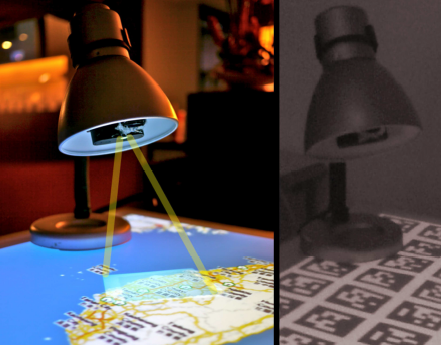
\includegraphics[width=0.5\columnwidth]{images/WeiChan2010_1.png}
\begin{center}
\footnotesize{
\textit{\thecimages. attēls. Infrasarkanās un redzamās gaismas projektors neredzamu marķieru projekcijām.}}
\end{center}
\end{center}
\end{samepage}

\par 
Neredzamus infrasarkanos kvadrātveida marķierus ir iespējams apslēpt arī vienkāršos, izdrukātos attēlos,
izmantojot pelēkos pustoņus, kurus starp attēla pikseļiem iejauc ar 3$\%$ koncentrāciju no visa attēla \cite{Hsi-ChunWang2008}.
Diemžēl šādi marķieri ir apslēpjami tikai gaišos attēlos, kā parādīts \prettyref{cimages:ChunWang2008_1} attēlā.

\refstepcounter{cimages}\label{cimages:ChunWang2008_1}
\vspace{10pt}
\begin{samepage}
\begin{center}
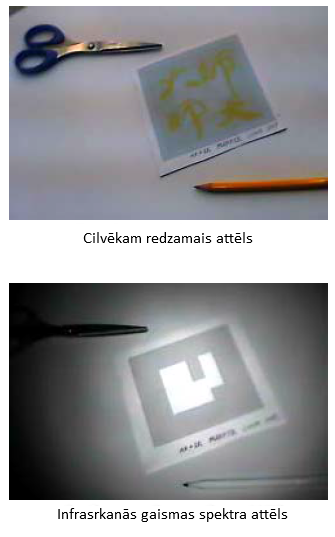
\includegraphics[width=0.3\columnwidth]{images/ChunWang2008_1.png}
\begin{center}
\footnotesize{
\textit{\thecimages. attēls. Pustoņos paslēpts infrasarkanās gaismas marķieris.}}
\end{center}
\end{center}
\end{samepage}


\refstepcounter{cimages}\label{cimages:ChunWang2008_2}
\vspace{10pt}
\begin{samepage}
\begin{center}
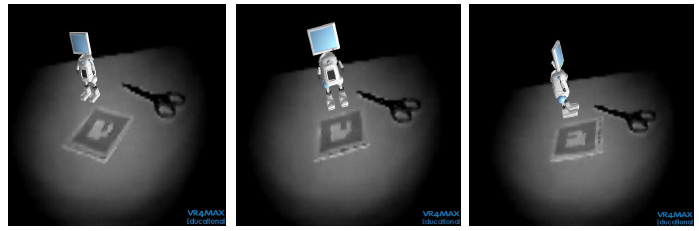
\includegraphics[width=0.7\columnwidth]{images/ChunWang2008_2.png}
\begin{center}
\footnotesize{
\textit{\thecimages. attēls. Infrasarkanās gaismas kvadrātveida marķieris virtuāla objekta pozicionēšanai telpā.}}
\end{center}
\end{center}
\end{samepage}

\par
Vēl neredzamus kvadrātveida marķierus var realizēt, izmantojot retroflektīvus marķierus jeb spoguļveida 
marķierus, kuri aktīvi neizstaro gaismu, bet atstaro uz tiem spīdošo gaismu, kas var būt arī infrasarkanajā
gaismas spektrā, padarot to atrašanu neredzamu cilvēka acij \cite{YusukeNakazato2004}. 
Šāda marķieru sistēma ir vienkārša un efektīva, taču nav adaptīva situācijām, kad telpā var būt
dažādi objekti ar vienādu kvadrātveida marķieri. Tāpat šie marķieri nevar pārraidīt kamerai nekādu
papildus dinamiski mainīgu informāciju.

\refstepcounter{cimages}\label{cimages:YusukeNakazato2004}
\vspace{10pt}
\begin{samepage}
\begin{center}
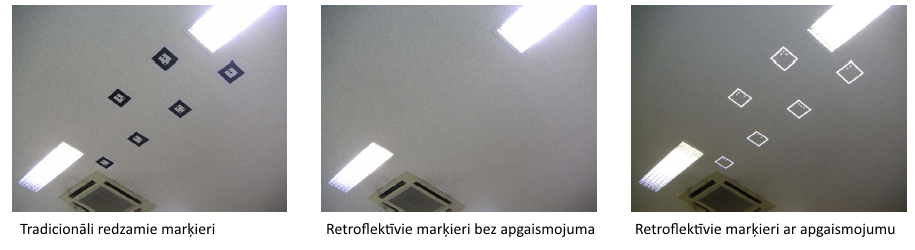
\includegraphics[width=0.8\columnwidth]{images/YusukeNakazato2004.png}
\begin{center}
\footnotesize{
\textit{\thecimages. attēls.}}
\end{center}
\end{center}
\end{samepage}

\par
Alternatīva metode neredzamu vai gaismekļos apslēptu marķieru sistēmas izveidei var tikt izveidota,
izmantojot kameras ekspozīcijas laiku un augstas frekvences (1-100 kHz) mirgojošas diodes. 
Amerikā veiktā pētījumā šādi marķieri tika apslēpti telpu gaismekļos, kuros cilvēka acs nepamana
mirgošanas izmaiņas \cite{Ye-ShengKuo2014}. Interesanti, ka arī telefona kamera ar zemu kadru frekvenci (50 Hz) nespēj
nolasīt visas mirgošanas izmaiņas, taču ir iespējams iegūt nepilnīgus attēlus atkarībā no
kameras kadra ekspozīcijas laika, no kuriem var nolasīt datus. Tādējādi ar vienu kadru var nolasīt
pat 8 un vairāk bitus. Diemžēl šādai sistēmai ir nepieciešams liels gaismu izstarojošais objekts 
vai augstas izšķirtspējas kamera. Šādu datu atkodēšana prasa arī lielākus skaitļošanas resursus. 
Pētījumā šī metode tika izmantota kameras pašlokalizācijas problēmas risināšanā, kur katrs gaismeklis
pārraidīja savu identifikatoru.

\refstepcounter{cimages}\label{cimages:ShengKuo2014_1}
\vspace{10pt}
\begin{samepage}
\begin{center}
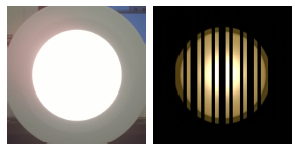
\includegraphics[width=0.5\columnwidth]{images/ShengKuo2014_1.png}
\begin{center}
\footnotesize{
\textit{\thecimages. attēls. Datu kodēšana marķieros, izmantojot kameras kadra ekspozīcijas laiku. Pa kreisi acij redzamais attēls. Pa labi kameras kadra attēls, pārraidot datus ar 1 kHz frekvenci, bet filmējot objektu ar 50 Hz frekvenci.}}
\end{center}
\end{center}
\end{samepage}

%%%%%%%%%%%%%%%%%%%%%%%%%%%%%%%%%%%%%%%%%%%%%%%%%%%%%%%%%%%%%%%%%%%%%%%%%%%%%%%%%%%%%%%%%%%%%%%%%%%%%%%%%%%%%%

\newpage
\section{Algoritms neredzamu marķieru sistēmai}\label{section_imaging}

\par
Šajā pētījumā piedāvātais risinājums fizisku objektu pozīciju noteikšanai telpā sastāv no infrasarkanās
stereo kameras un aktīviem infrasarkaniem marķieriem. Šie marķieri ir implementēti kā LED infrasarkanās
gaismas diodes, kuras izstaro gaismu 850nm gaismas viļņa garumā, kuru savukārt ir spējīga uztvert
Leap Motion kamera, kura izmanto 850nm infrasarkanās gaismas filtru. Lai aprakstītu objekta atrašanās
vietu, telpā ir nepieciešams iegūt attēlu abās stereo kameras pusēs no vismaz vienas diodes. Savukārt,
lai iegūtu objekta orientāciju telpā, ir nepieciešams iegūt vismaz 3 diožu vienlaicīgu attēlojumu abās
kamerās. Neredzamās gaismas diožu intensitāti kontrolē Arduino mikro-kontrolieris, kas pārraida, ieslēdzot 
un izslēdzot gaismas diodes to identifikācijas numurus ar 37 Hz frekvenci. 

\par

Datu nolasīšanas algoritma izpildāmie soļi:
\begin{enumerate}

\item Katrai acij uzkrāt attēlu buferi no Leap Motion (izpildīt pavedienos jeb paralēlos procesos)
\item Samazināt attēla rezolūciju, lai nodrošinātu ātrdarbību (izpildīt pavedienos jeb paralēlos procesos)
\item Adaptīvi atrast mirgojošos punktus (izpildīt pavedienos jeb paralēlos procesos):
\begin{enumerate}
\item Iteratīvi apskatīt intensitātes spektru katram attēlam, pa slāņiem, no 5 - 255 intensitātei ar 10 gradāciju soli,
lai novērstu apgaismojuma ietekmi uz signāla pārraidi.
\item Veikt attēla izpludināšanu, izmantojot Gausa sapludināšanas filtru.
\item Veikt attēla filtrāciju ar Mediānas filtru.
\item Atrast kontūras un apgabalus, kuri varētu būt gaismas diodes.
\item Filtrēt kontūras pēc laukuma.
\item Atrast kontūru centrus.
\item Saglabāt kontūru statusu. Ja eksistē, tad bita vērtība ir 1, ja neeksistē, tad 0.
\item Atkodēt datus, izmantojot Mančestras kodēšanu, kas nodrošina precīzam laikam nepiesaistītu datu pārraidi.
\item Veikt datu atkļūdošanu dažādus algoritmus, kuri aprakstīti \ref{section_protocol}.nodaļā.
\end{enumerate}
\item Salīdzināt iegūtos digitālos identifikatorus un klasificēt kontūras. 
\item Filtrēt klasificētās kontūras, izmantojot Kalmana vai daļiņu filtrus.
\item Iegūt kontūru pozīcijas no kameras attēla plaknes 3 dimensiju telpas koordinātēs. Izmantotie algoritmi aprakstīti \ref{section_stereo}.nodaļā.
\item Pēc kameras pārvietojuma datu iegūšanas (odometrijas), projicēt 3D koordinātes uz 
2D kameras attēla, lai uzlabotu precizitāti. Kameras odometrijas datus iegūst no Oculus Rift sensoriem un statiskās infrasarkanās gaismas kameras, kura nodrošina precīzu pārvietojuma noteikšanu tieši ekrānam, kas ir piestiprināts pie galvas
un pie kura, savukārt, ir piestiprinātas Leap Motion kameras.

\end{enumerate}

\par
Attēla apstrāde tiek sākta ar mediānas filtra pielietošanu. Mediānas filtra algoritms parādīts \prettyref{cimages:4_a1}. attēlā. 
Algoritms apskata definētu skaitu kaimiņu pikseļus visos virzienos katram pikselim $g(x,y)$ un sakārtot tos secīgi, lai tas saturētu centrālo vērtību.
Mediānas algoritma apgabals tika izvēlēts 2 blakus esošo pikseļu robežās.

\refstepcounter{cimages}\label{cimages:4_a1}
\vspace{10pt}
\begin{center}
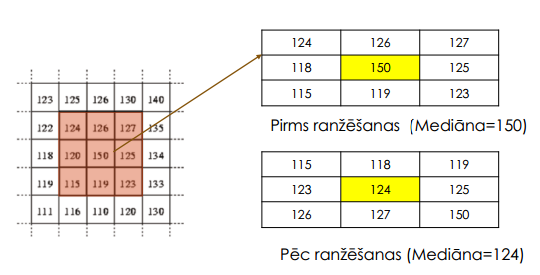
\includegraphics[width=0.6\columnwidth]{images/4_a1.png}
\begin{center}
\footnotesize{
\textit{\thecimages. attēls. Mediānas algoritma darbību piemērs.}}
\end{center}
\end{center}


\refstepcounter{cimages}\label{cimages:median}
\vspace{10pt}
\begin{samepage}
\begin{center}
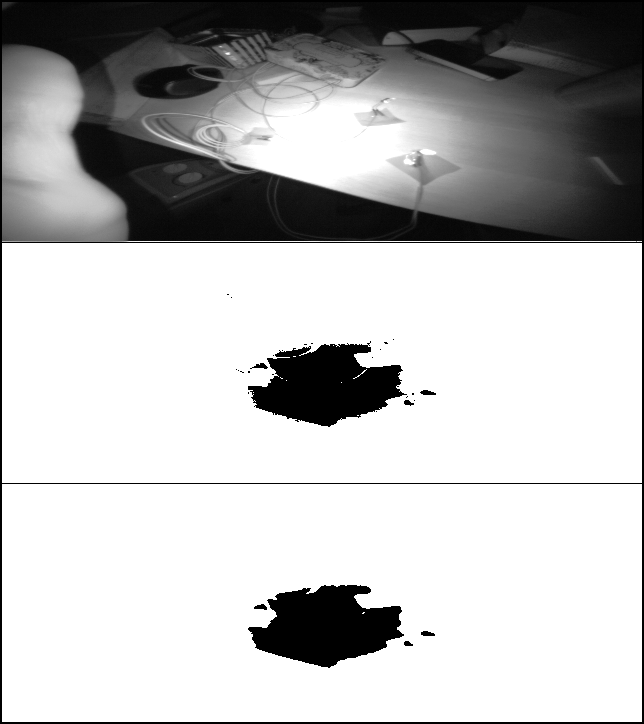
\includegraphics[width=1\columnwidth]{images/median.png}
\begin{center}
\footnotesize{
\textit{\thecimages. attēls. Augstākais no attēliem ir oriģinālais attēls, kas tiek iegūts no Leap Motion kreisās kameras. Otrais attēls ir binārais attēls ar intensitātes filtru bez mediānas filtra. Trešais attēls ir binārais attēls ar intensitātes filtru, izmantojot mediānas filtru pirms intensitātes robežas filtra.}}
\end{center}
\end{center}
\end{samepage}

\par Pēc tam attēla izmēri tika samazināti uz pusi. Samazināšanas koeficients tika izvēlēts eksperimentāli,
tā, lai marķieru izmēri 2 m attālumā aizņemtu vismaz vienu pikseli pēc attēla samazināšanas. Šis solis ir ārkārtīgi
svarīgs, jo neskatoties uz to, ka katra attēla apstrāde notiek paralēlos procesos, tomēr pilna izmēra 640x240 pikseļu attēla apstrāde ar 111Hz frekvenci abām kamerām reālā laikā
prasa pārāk daudz skaitļošanas resursu. Savukārt, izmantojot 320x120 pikseļu izmēra attēlu ir iespējams nodrošināt attēlu apstrādi un datu signālu apstrādi reālā laikā,
izmantojot pētījumā pielietoto datortehniku.

\refstepcounter{cimages}\label{cimages:scaling}
\vspace{10pt}
\begin{samepage}
\begin{center}
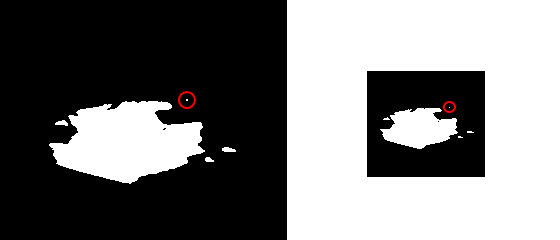
\includegraphics[width=1\columnwidth]{images/scaling.png}
\begin{center}
\footnotesize{
\textit{\thecimages. attēls. Kreisā pusē oriģinālā izmēra attēls, bet labajā pusē samazināta izmēra attēls, kurā arī iespējams saskatīt marķiera pikseļus.}}
\end{center}
\end{center}
\end{samepage}

\par
Lai segmentētu attēlā redzamos infrasarkanos marķierus, svarīga algoritma sastāvdaļa ir izslēgt vides apgaismojuma ietekmi
uz datu pārraides kvalitāti. Apgaismojuma ietekmi var mazināt, saglabājot katrā iterācijā visus marķieru kandidātus
pa 10 gradāciju vērtību intensitātes slāņiem no 5-255 (krāsu intensitāte pieejama baita robežās). 
Intensitātes filtrs pikseļiem, kuru vērtības ir lielākas par apakšējo gradācijas slieksni, bet mazākas par augšējo gradāciju slieksni, piešķir vērtību "1", bet pikseļiem, kas ir zem šī sliekšņa, piešķir vērtību 0.

\refstepcounter{cimages}\label{cimages:filter}
\vspace{10pt}
\begin{samepage}
\begin{center}
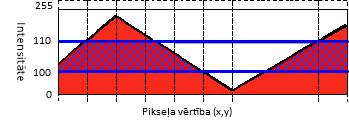
\includegraphics[width=0.5\columnwidth]{images/filter.png}
\begin{center}
\footnotesize{
\textit{\thecimages. attēls. Binārais attēla filtrs ar intensitāšu gradāciju soļiem.}}
\end{center}
\end{center}
\end{samepage}
\newpage

Ja marķiera kandidāts konkrētajā slānī pārraida datus, tad
tām jābūt redzamam, un šim kandidātam slānī jāpiešķir pilna bita vērtība, bet ja tas neraida datus, tad tam piešķir tukša bita vērtību.
Kadra attēlu kadra kandidātu vērtības tiek saglabātas virknēs, kuras tālāk izmanto signālu apstrādē datu slāņa komunikācijas protokolā, kas
aprakstīts \ref{section_protocol}.nodaļā.

\refstepcounter{cimages}\label{cimages:theresholds}
\vspace{10pt}
\begin{samepage}
\begin{center}
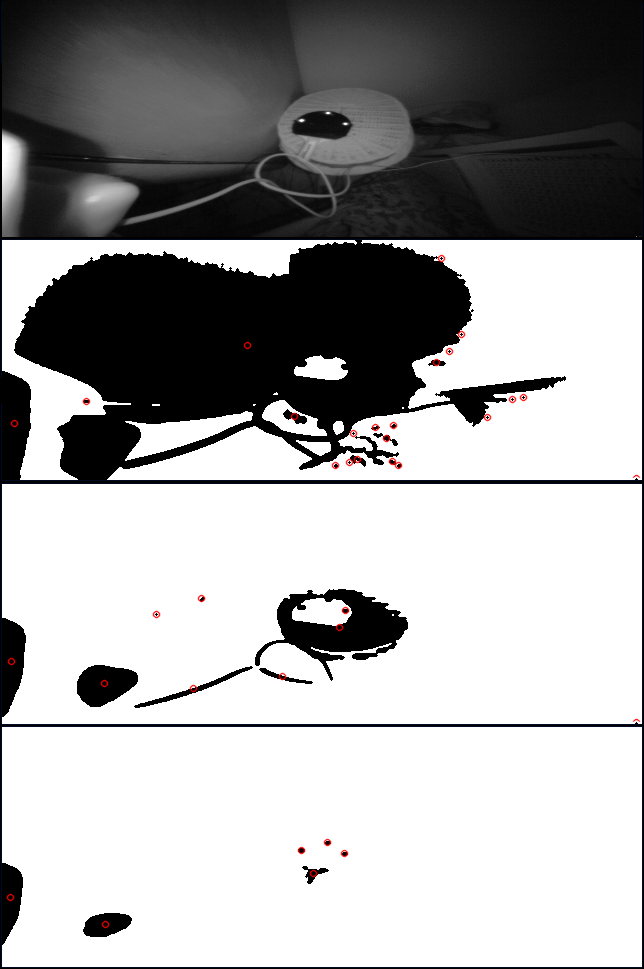
\includegraphics[height=1.2\columnwidth]{images/theresholds.png}
\begin{center}
\footnotesize{
\textit{\thecimages. attēls. Pakāpeniska pikseļu intensitātes filtrēšana pa 10 intensitāšu gradāciju vērtību slāņiem. Attēlos ir atzīmēti visas atrastās kontūras.}}
\end{center}
\end{center}
\end{samepage}
\newpage

\par
Marķieru kandidātu kontūru un to centru atrašanai tika pielietots S.Suzuki algoritms topoloģisku kontūru noteikšanai \cite{SatoshiSuzuki1985}.
Tas tika izmantots, lai pārbaudītu vai diodes kontūra nesatur citas iekšējas kontūras, kas nevarētu tur atrasties
diodes attēla gadījumā, kā arī šis algoritms ir implementēts OpenCV bibliotēkā, kas tika izmantota attēlu apstrādē.

Algoritma izpildāmie soļi:
\begin{enumerate}
\item[1] Tiek saņemts binārs attēls.
\item[2] Kontūru skaitītājs uzstādīts $N=1$.
\item[3] Pārvieto kursoru pa y rindām uz leju un x asi pa labi, līdz iegūst attēla pikseli
\item[4.1] Ja $f_{x,y} = 1$ un $f_{x-1,y}=0$. Tiek palielināta $N$ vērtība un tiek saglabāti punkti $A_{x,y}$, $B_{x-1,y}$.
\item[4.2] Ja atrod jau apskatītu pikseli $f_{x,y} \geqslant 1$ un $f_{x+1,y}=0$, tad pieņem, ka ir atrasts apakš-kontūrs, kuram
saglabā punktus $A_{x,y}$ un $B_{x+1,y}$ palielina $N$ vērtību. Jauno vērtību reģistrē kontūru koka struktūrā kā apakškopu.
\item[5] Sākot no punkta $A_{x,y}$, seko kontūrai pa x un y asīm pēc nosacījumiem sekojošos soļos. Apejot kontūru, to var saglabāt hierarhijā atsevišķā struktūrā,
jo kopējā pikseļu matrica pēc algoritma izpildes nedos skaidru informāciju par kontūru robežām, bet no tās varēs iegūt informāciju tikai par iekšējo kontūru skaitu.
\item[6.1] Ap punktu $A$ apskata 8 kaimiņu pikseļus pulksteņrādītāja virzienā, sākot no pikseļa $B$. Pirmais pikselis, kura
vērtība nav 0, tiek uzstādīts kā $C$ ar atrasto pozīciju. Ja neviens pikselis nav atrasts, tad tā vērtību uzstāda kā $-N$ un jādodas uz 3.soli. 
\item[6.2] $B \leftarrow C$ un $D \leftarrow A$
\item[6.3] Ap punktu $D$ apskata 8 kaimiņu pikseļus pretēji pulksteņrādītāja virzienam, sākot no pikseļa $B$. 
Pirmā pikseļa pozīcija, kas nav ar vērtību 0, tiek saglabāta kā $E$. Ir nepieciešams arī saglabāt apskatītos pikseļus līdz $E$, kas būs nepieciešami nākamajos apakš-soļos.
\item[6.3.1] Ja $D{x+1,y}$ vērtība ir 0 un $D{x+1,y}$ tika apskatīts 6.3 solī līdz $E$ pikselim, tad $D_{x,y} = -N$
\item[6.3.2] Ja $D{x+1,y}$ vērtība nav 0 un $D{x+1,y}$ netika apskatīts 6.3 solī līdz $E$ pikselim, tad $D_{x,y} = N$
\item[6.3.3] Pretējā gadījumā kā 6.3.1 un 6.3.2 $D$ vērtība netiek mainīta.
\item[6.4] Ja $E = A$ un $D = C$ (nonākam sākumpunktā) tad reģistrēt kontūru un doties uz 3. soli. Pretējā gadījumā 
pozīcijas tiek mainītas uz $B \leftarrow D$ un $D \leftarrow E$, un jādodas uz 6.1 soli.
\item[7] Algoritms beidz darbu, sasniedzot attēla apakšējo labo stūri iterācijā, kura aprakstīta 3.solī.
\end{enumerate}

\refstepcounter{cimages}\label{cimages:contour_algo}
\vspace{10pt}
\begin{samepage}
\begin{center}
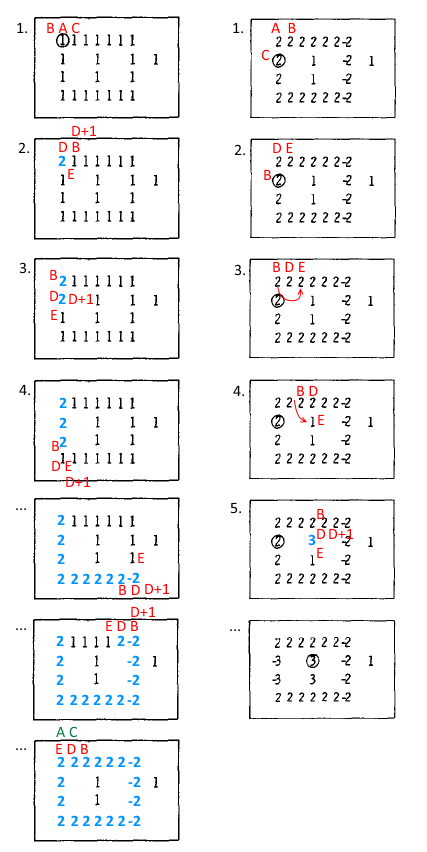
\includegraphics[height=0.95\columnwidth]{images/contour_algo.png}
\begin{center}
\footnotesize{
\textit{\thecimages. attēls. Pirmās kontūras atrašana, izmantojot S.Suzuki algoritmu (pa kreisi). Pirmās apakš-kontūras atrašana (pa labi).}}
\end{center}
\end{center}
\end{samepage}

Algoritma princips ir secīgi pulksteņrādītāja virzienā apskatīt kaimiņu pikseļus, tādējādi
iegūstot kontūras un, izmantojot arī īpašību mainīt kustības virzienu, apskatot arī apakš-kontūras.
Lai iegūtu vairākus apakš-kontūras tiek izmantota numerācijas metode, izmantojot algoritmā definētos nosacījumus.

\refstepcounter{cimages}\label{cimages:Suzuki1985_1}
\vspace{10pt}
\begin{samepage}
\begin{center}
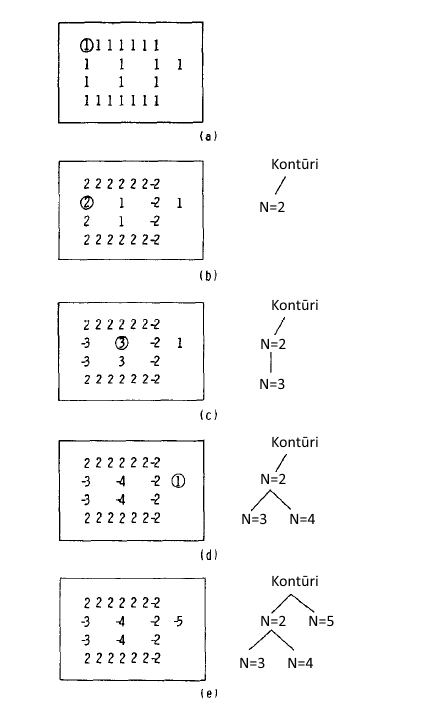
\includegraphics[height=0.85\columnwidth]{images/Suzuki1985_1.png}
\begin{center}
\footnotesize{
\textit{\thecimages. attēls. Iegūtās kontūras matrica un hierarhija, izmantojot S.Suzuki algoritmu.}}
\end{center}
\end{center}
\end{samepage}

Vēl, bez pētījumā izmantotā algoritma, var pielietot virkni citu algoritmu kontūras un tās centra noteikšanai 
\cite{LingfeiZhang2008} \cite{KeshengWu2005} \cite{YuhaiLi2010} \cite{VictorM.A.Oliveira2010}.
Ģeometriskais centrs, kas tiek uzskatīts par marķiera centru, tiek iegūts no aptverošā taisnstūra centra.
Aptverošo taisnstūri veido kontūras tālāko stūru vektoru pozīcijas.

%TODO circularity size

\newpage
\subsection{Infrasarkano marķieru implementācija}\label{section_implement}

\par 
Infrasarkanie marķieri tika izveidoti dažādās konfigurācijās atkarībā no testos izmantotā objekta
ģeometriskajām īpašībām. Objekti, kā ēkas platforma (\prettyref{cimages:uzd1model}. attēlā) vai galda tenisa
rakete (\prettyref{cimages:IMG_4364}. attēlā) tika implementēti, izmantojot plakni, kuru definē 3 diožu pozīcijas
telpā. Savukārt telpisks objekts, kā violetā rotaļlieta (\prettyref{cimages:begemot_sample_1}. attēlā) tika 
implementēta, izmantojot 5 gaismas diodes, ļaujot atpazīt objekta pozīciju un orientāciju no jebkura 
leņķa, ja rotaļlieta ir novietota uz virsmas, kā parādīts attēlā. 

\refstepcounter{cimages}\label{cimages:house_example}
\vspace{10pt}
\begin{samepage}
\begin{center}
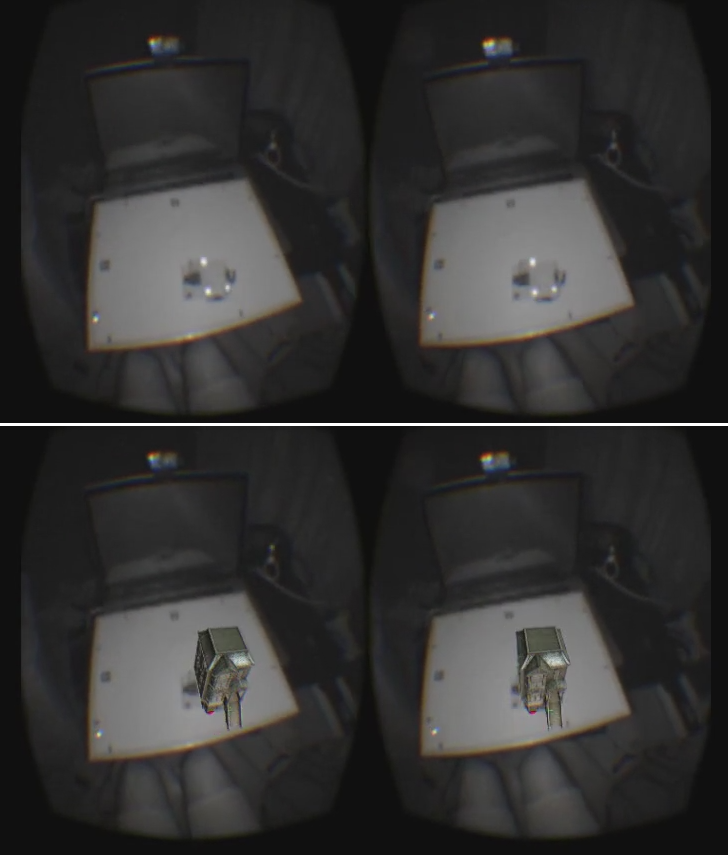
\includegraphics[width=0.6\columnwidth]{images/house_example.png}
\begin{center}
\footnotesize{
\textit{\thecimages. attēls. Ēkas platformas pozīcija un orientācija paplašinātajā realitātē, izmantojot neredzamos infrasarkanos marķierus .}}
\end{center}
\end{center}
\end{samepage}

\refstepcounter{cimages}\label{cimages:IMG_4362}
\vspace{10pt}
\begin{samepage}
\begin{center}
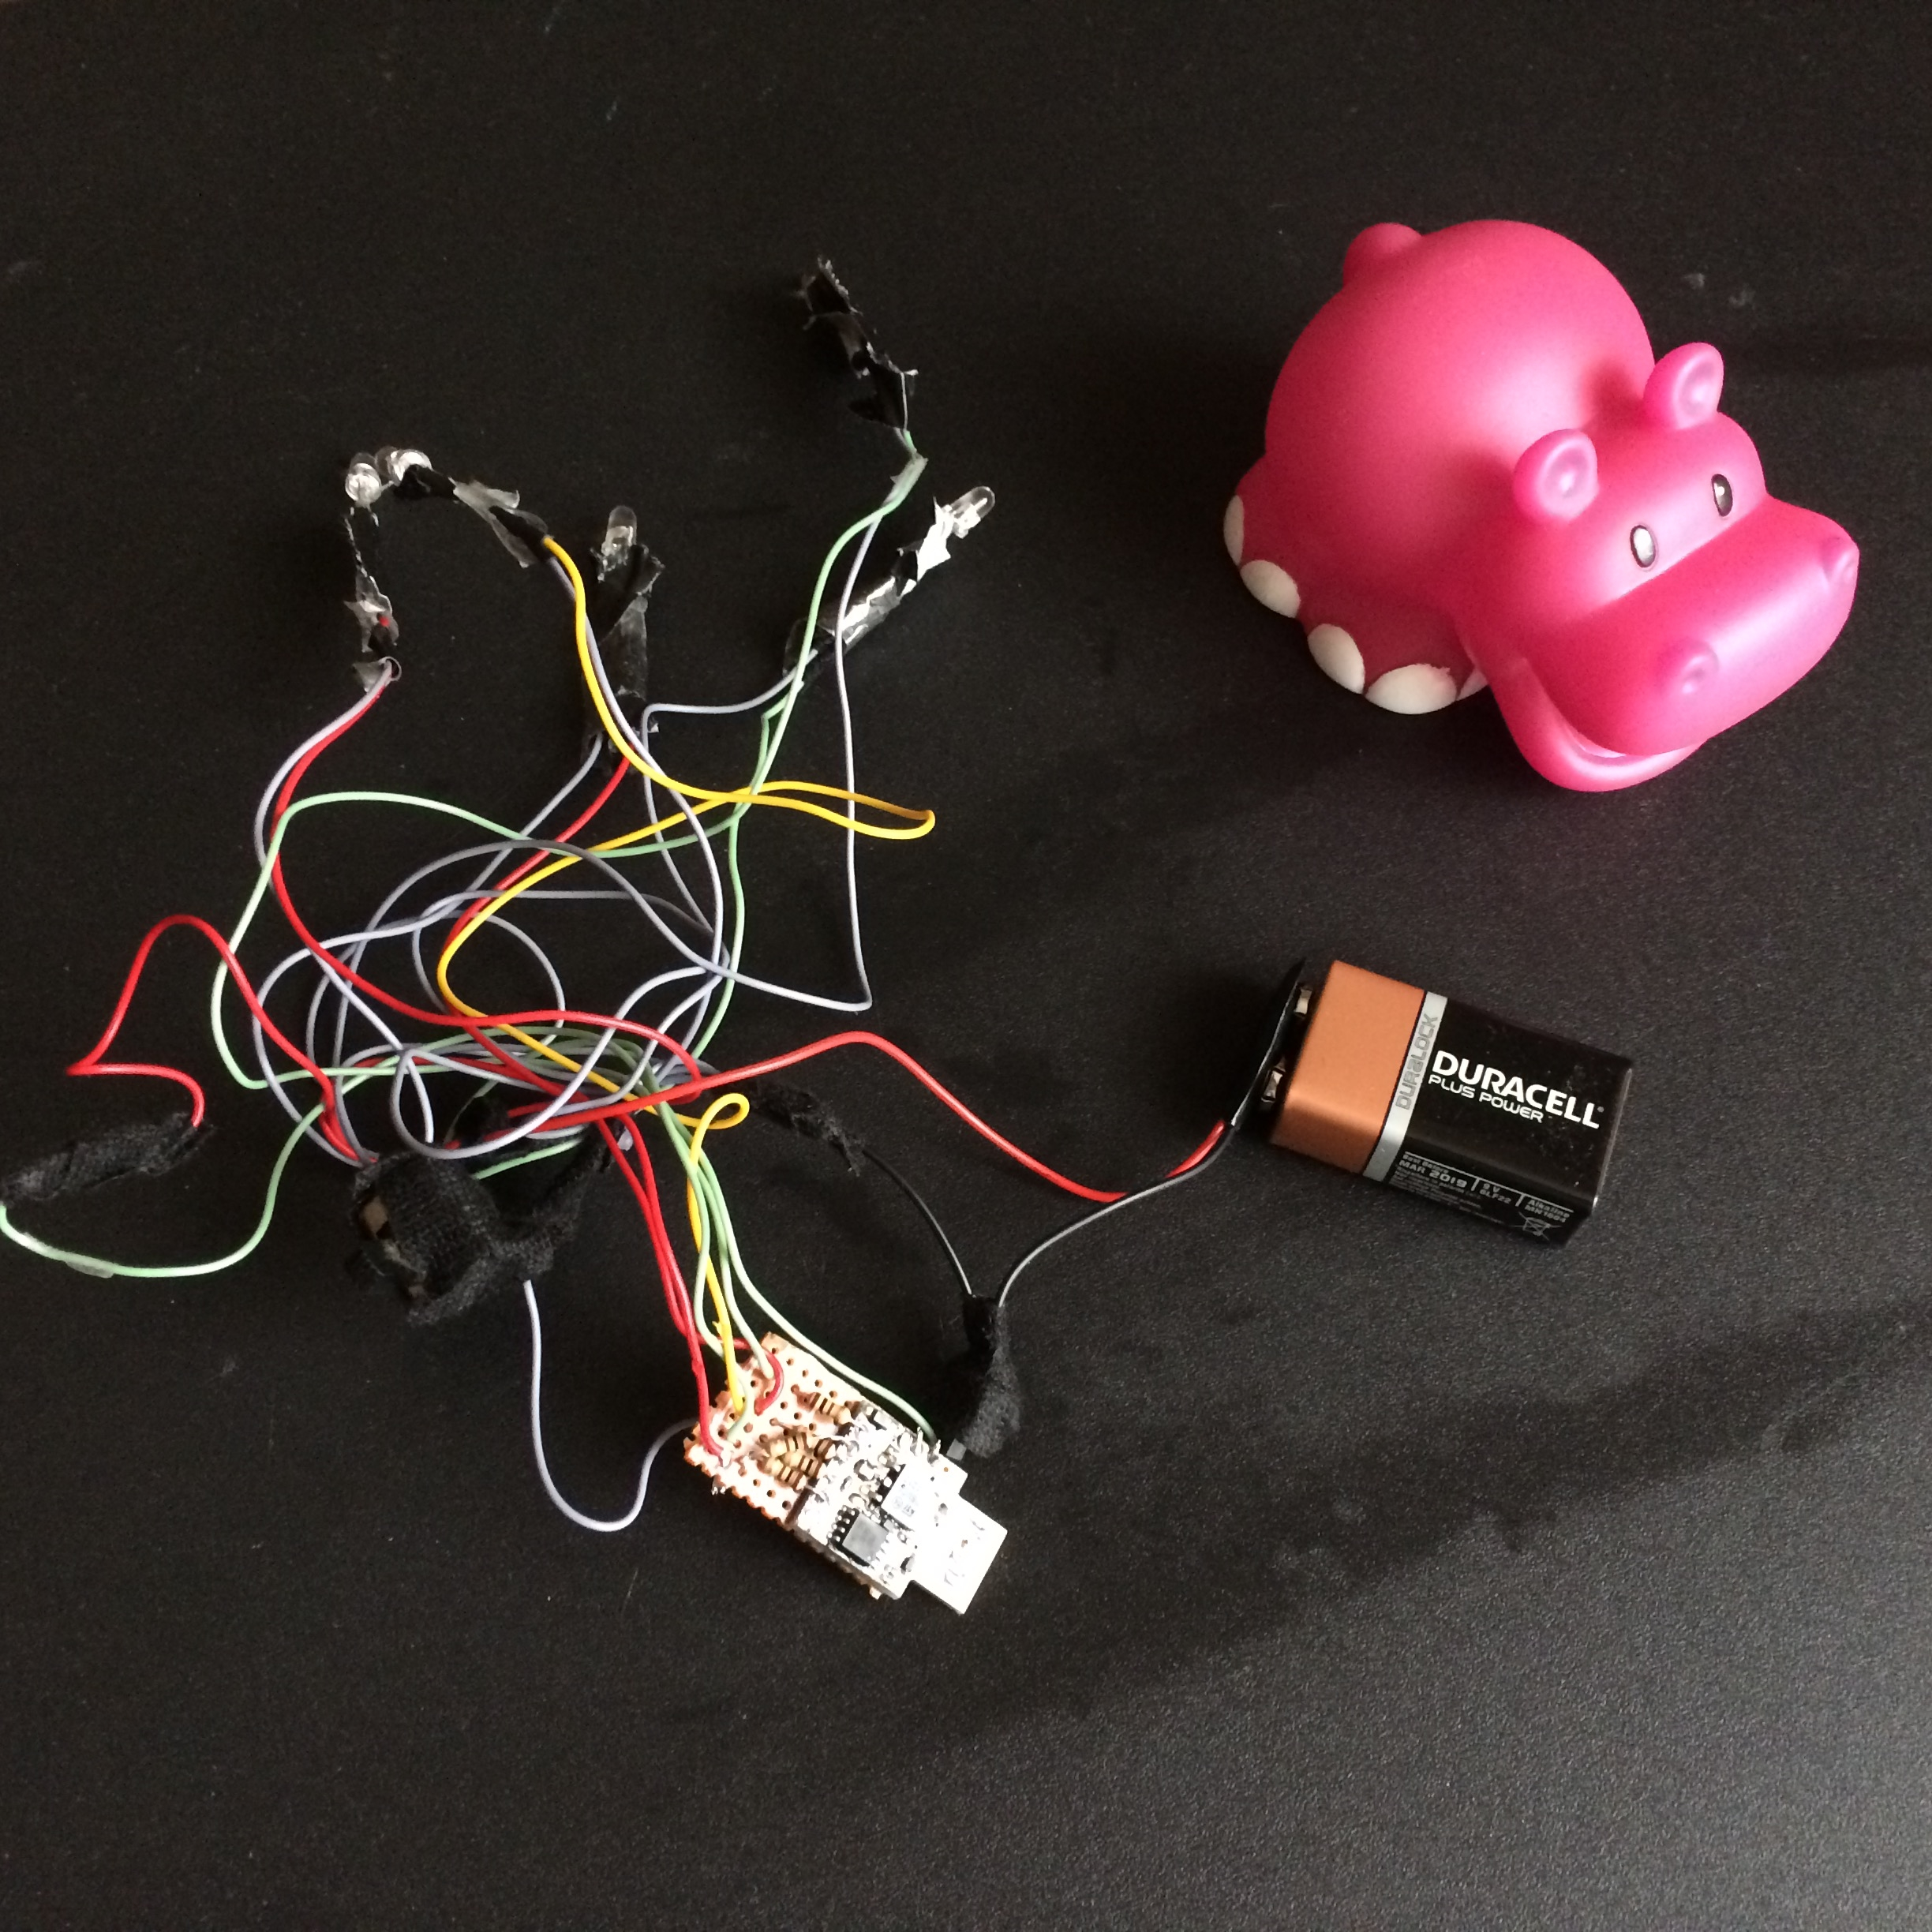
\includegraphics[width=0.6\columnwidth]{images/IMG_4362.JPG}
\begin{center}
\footnotesize{
\textit{\thecimages. attēls. Ardunio shēma ar infrasarkanās gaismas diodēm.}}
\end{center}
\end{center}
\end{samepage}

\refstepcounter{cimages}\label{cimages:begemot_sample_1}
\vspace{10pt}
\begin{samepage}
\begin{center}
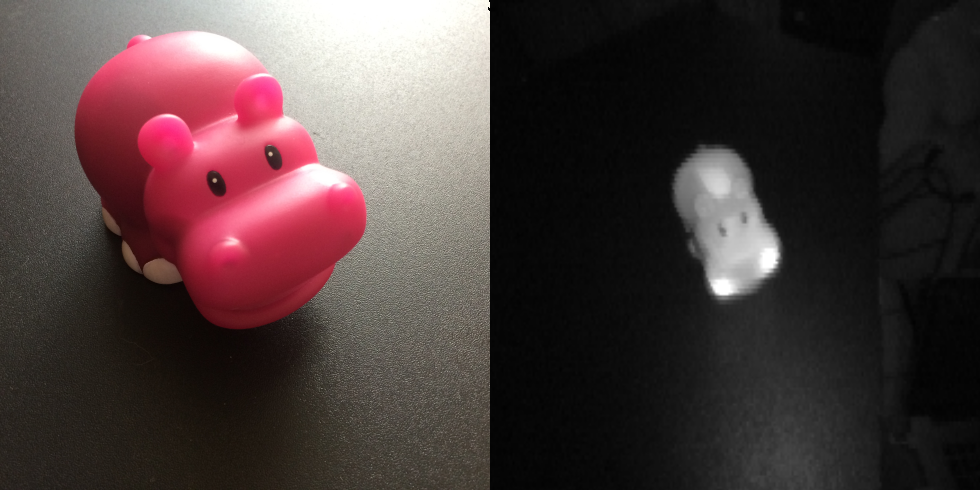
\includegraphics[width=0.6\columnwidth]{images/begemot_sample_1.png}
\begin{center}
\footnotesize{
\textit{\thecimages. attēls. Rotaļlieta ar infrasarkanajiem gaismas marķieriem, kuri nav redzami RGB attēlā pa kreisi.}}
\end{center}
\end{center}
\end{samepage}

\par
Atšķirībā no infrasarkanās gaismas tālvadības pultīm, kuras darbojas ar 33 - 40 kHz frekvencēm \cite{ThibautRaharijaona2010}, šajā pētījumā
piedāvātā sistēma ir ievērojami jūtīgāka pret datu pārraides traucējumiem. 
Šī iemesla dēļ komunikācijas protokols fiziskajā līmenī izveidots, lai iegūtie dati saturētu
pēc iespējas mazāk kļūdu, un tos būtu iespējams izlabot. Vēl atšķirībā no televīzijas un citu
ierīču tālvadības pultīm, kur tiek izmantotas pārsvarā 950nm viļņa garuma diodes,
piedāvātajā sistēmā tika izmantotas 850nm viļņa garuma diodes, jo Leap Motion kamerām ir
gaismas filtrs tieši šādai gaismas viļņa frekvencei.

\newpage
\par
Implementējot marķieru sistēmu, tika izmantota bezmaksas programmatūra un plaša patēriņa tirgū
pieejami elektroniskie komponenti, kā parādīts \prettyref{ctables:hardware}., \prettyref{ctables:software}. tabulās.

\begin{samepage}
\begin{table}[h]
\centering
\begin{tabular}{|l|l|l|}
\hline
\rowcolor[HTML]{D0D0D0} 
Nosaukums                    & Apraksts                                                                                                                 & Skaits \\ \hline
Ardunio Nano ATmega328       & 16MHz, 5V                                                                                                                & 2      \\ \hline
DigiSpark Digistump B        & 16.5MHz, 5V                                                                                                              & 1      \\ \hline
Infrasarkānās gaismas diodes & \begin{tabular}[c]{@{}l@{}}850nm, 1.5V, \\ 90mW, 50mA\end{tabular}                                                       & 3 * 2 + 5  \\ \hline
Leap Motion                  & \begin{tabular}[c]{@{}l@{}}Infrasarkanās gaismas stereo kamera\\ ar 850nm filtru\end{tabular}                            & 1      \\ \hline
Oculus Rift DK2              & \begin{tabular}[c]{@{}l@{}}Pie galvas piestiprināms virtuālās\\ realitātes ekrāns ar pozicionēšanas sistēmu\end{tabular} & 1      \\ \hline
MacBook Pro                  & \begin{tabular}[c]{@{}l@{}}nVidia GTM750 2GB, 16GB DDR3 RAM, \\ Intel i7 2.5 GHz (4 core)\end{tabular}                   & 1      \\ \hline
\end{tabular}
\end{table}
\vspace{-0.5cm}
\refstepcounter{ctables}\label{ctables:hardware}
\begin{center}
\footnotesize{
\textit{\thectables. tabula. Pētījumā izmantotā elektrotehnika.}}
\end{center}
\end{samepage}

\begin{samepage}
\begin{table}[h]
\centering
\begin{tabular}{|l|l|}
\hline
\rowcolor[HTML]{D0D0D0} 
Nosaukums             & Apraksts                                                                                                                                                    \\ \hline
Microsoft Windows 8.1 & \begin{tabular}[c]{@{}l@{}}Operētājsistēma izstrādei un testēšanai.\\ Tika izvēlēta, jo Oculus Rift piedāvā\\ paaugstinātas veiktspējas dzini.\end{tabular} \\ \hline
Unity 5               & Grafiskais dzinis iegūtās scēnas attēlošanai.                                                                                                               \\ \hline
MonoDevelop 5         & \begin{tabular}[c]{@{}l@{}}Programmatūras izstrāde datu saņemšanai\\ tika veikta, izmantojot C\# valodu.\end{tabular}                                        \\ \hline
Ardunio IDE           & \begin{tabular}[c]{@{}l@{}}Programmatūras izstrāde datu pārraidei\\ tika veikta, izmantojot C valodu.\end{tabular}                                          \\ \hline
Emgu / OpenCV 2.4     & Bibliotēka grafiskai apstrādei, izmantojot GPU.                                                                                                             \\ \hline
Oculus Rift SDK       & Oculus Rift iekārtas saskarnes bibliotēka.                                                                                                                  \\ \hline
Leap Motion SDK       & Leap Motion iekārtas saskarnes bibliotēka.                                                                                                                  \\ \hline
nVidia CUDA SDK       & Vispārīgo ēnotāju saskarnes bibliotēka, izmantojot GPU.                                                                                                                  \\ \hline
XZImg			      & \begin{tabular}[c]{@{}l@{}}Bibliotēka tradicionālo redzamo\\ marķieru pozīciju un orientācijas noteikšanai.\end{tabular}                                                                                                                   \\ \hline
\end{tabular}
\end{table}
\vspace{-0.5cm}
\refstepcounter{ctables}\label{ctables:software}
\begin{center}
\footnotesize{
\textit{\thectables. tabula. Pētījumā izmantotā programmatūra.}}
\end{center}
\end{samepage}

\refstepcounter{cimages}\label{cimages:LeapVR_schem.png}
\vspace{10pt}
\begin{samepage}
\begin{center}
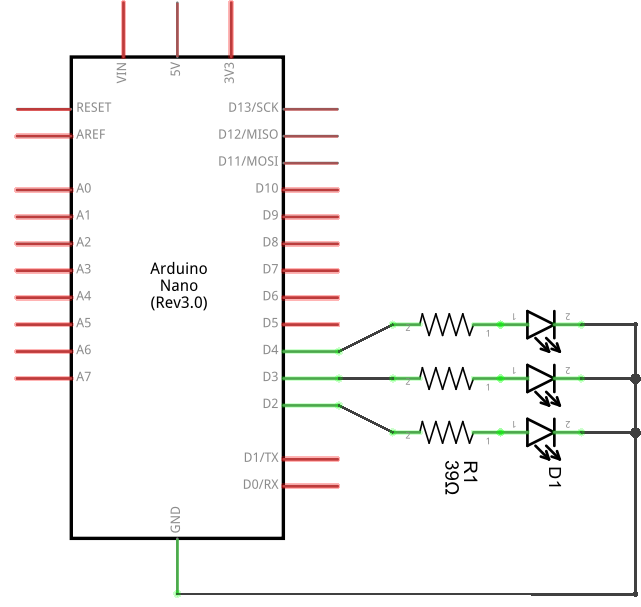
\includegraphics[width=0.5\columnwidth]{images/LeapVR_schem.png}
\begin{center}
\footnotesize{
\textit{\thecimages. attēls. Ardunio shēma, izmantojot infrasarkanās gaismas diodes marķiera pozīcijas \\ un orientācijas noteikšanai. Galda tenisa raketes shēma ar 3 diodēm.}}
\end{center}
\end{center}
\end{samepage}

\par
Marķieru sistēmas atpazīšanas programma ir implementēta .net 3.5 satvarā C\# valodā, 
izmantojot vairākus paralēlus pavedienus kā parādīts
\prettyref{cimages:threading}. attēlā. Attēlu un signālu apstrāde notiek 
pētījumā izmantotajos piemēros 2 paralēlos pavedienos jeb paralēlos procesos, katrai acij, taču
to skaitu var palielināt atkarībā no pieejamo procesoru skaita.
Attēlu apstrādes algoritmi tiek veikti, izmantojot OpenCV, kas kompilēts ar
nVidia CUDA atbalstu, lai nodrošinātu papildus pavedienu izmantošanu grafiskajā procesorā.

\refstepcounter{cimages}\label{cimages:threading}
\vspace{10pt}
\begin{samepage}
\begin{center}
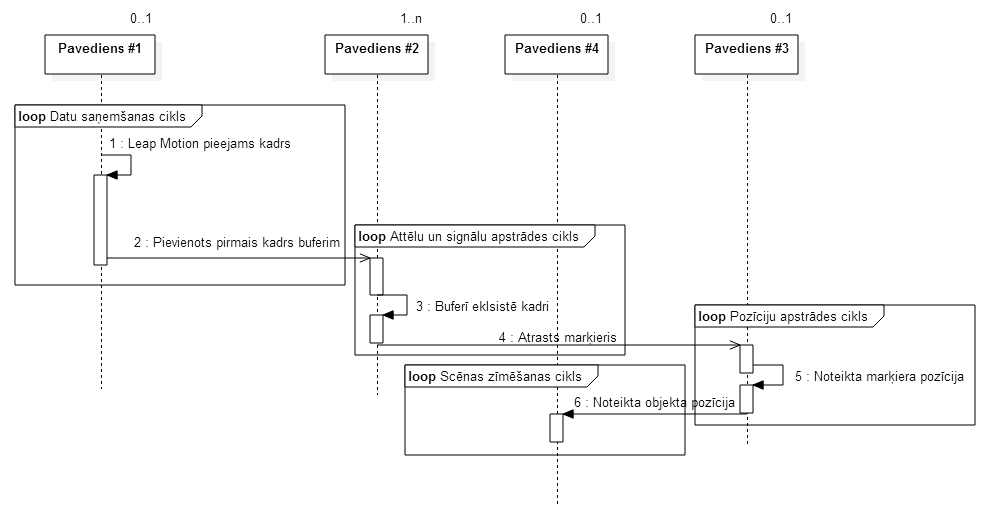
\includegraphics[width=0.9\columnwidth]{images/threading.png}
\begin{center}
\footnotesize{
\textit{\thecimages. attēls. Sistēmā izmantoto pavedienu jeb paralēlo procesu diagramma.}}
\end{center}
\end{center}
\end{samepage}

%TODO Li-Fi 

\newpage

Pētījuma ietvaros tika izveidota interaktīvas spēles programma, izmantojot galda tenisa raketi un paplašināto
realitāti. Spēlētāja virzienā lido galda tenisa bumbiņas, un tās spēlētājam ir jāatsit, izmantojot galda tenisa
raketi, kura aprīkota ar aktīviem infrasarkaniem marķieriem. Tā kā rakete strauji pārvietojas un maina
orientāciju telpā, šī programma labi demonstrē marķieru lokalizācijas veiktspēju reālā laikā.
Tenisa spēles un citu piemēru darbība ir iefilmēta video, kuri ir pieejami interneta vietnēs: \\
\url{http://tiny.cc/cp7myx} \\ \url{https://www.youtube.com/playlist?list=PLehOXo4NfxeVIWagwmKnIfyaVQdJqy8Xg}

\refstepcounter{cimages}\label{cimages:IMG_4364}
\vspace{10pt}
\begin{samepage}
\begin{center}
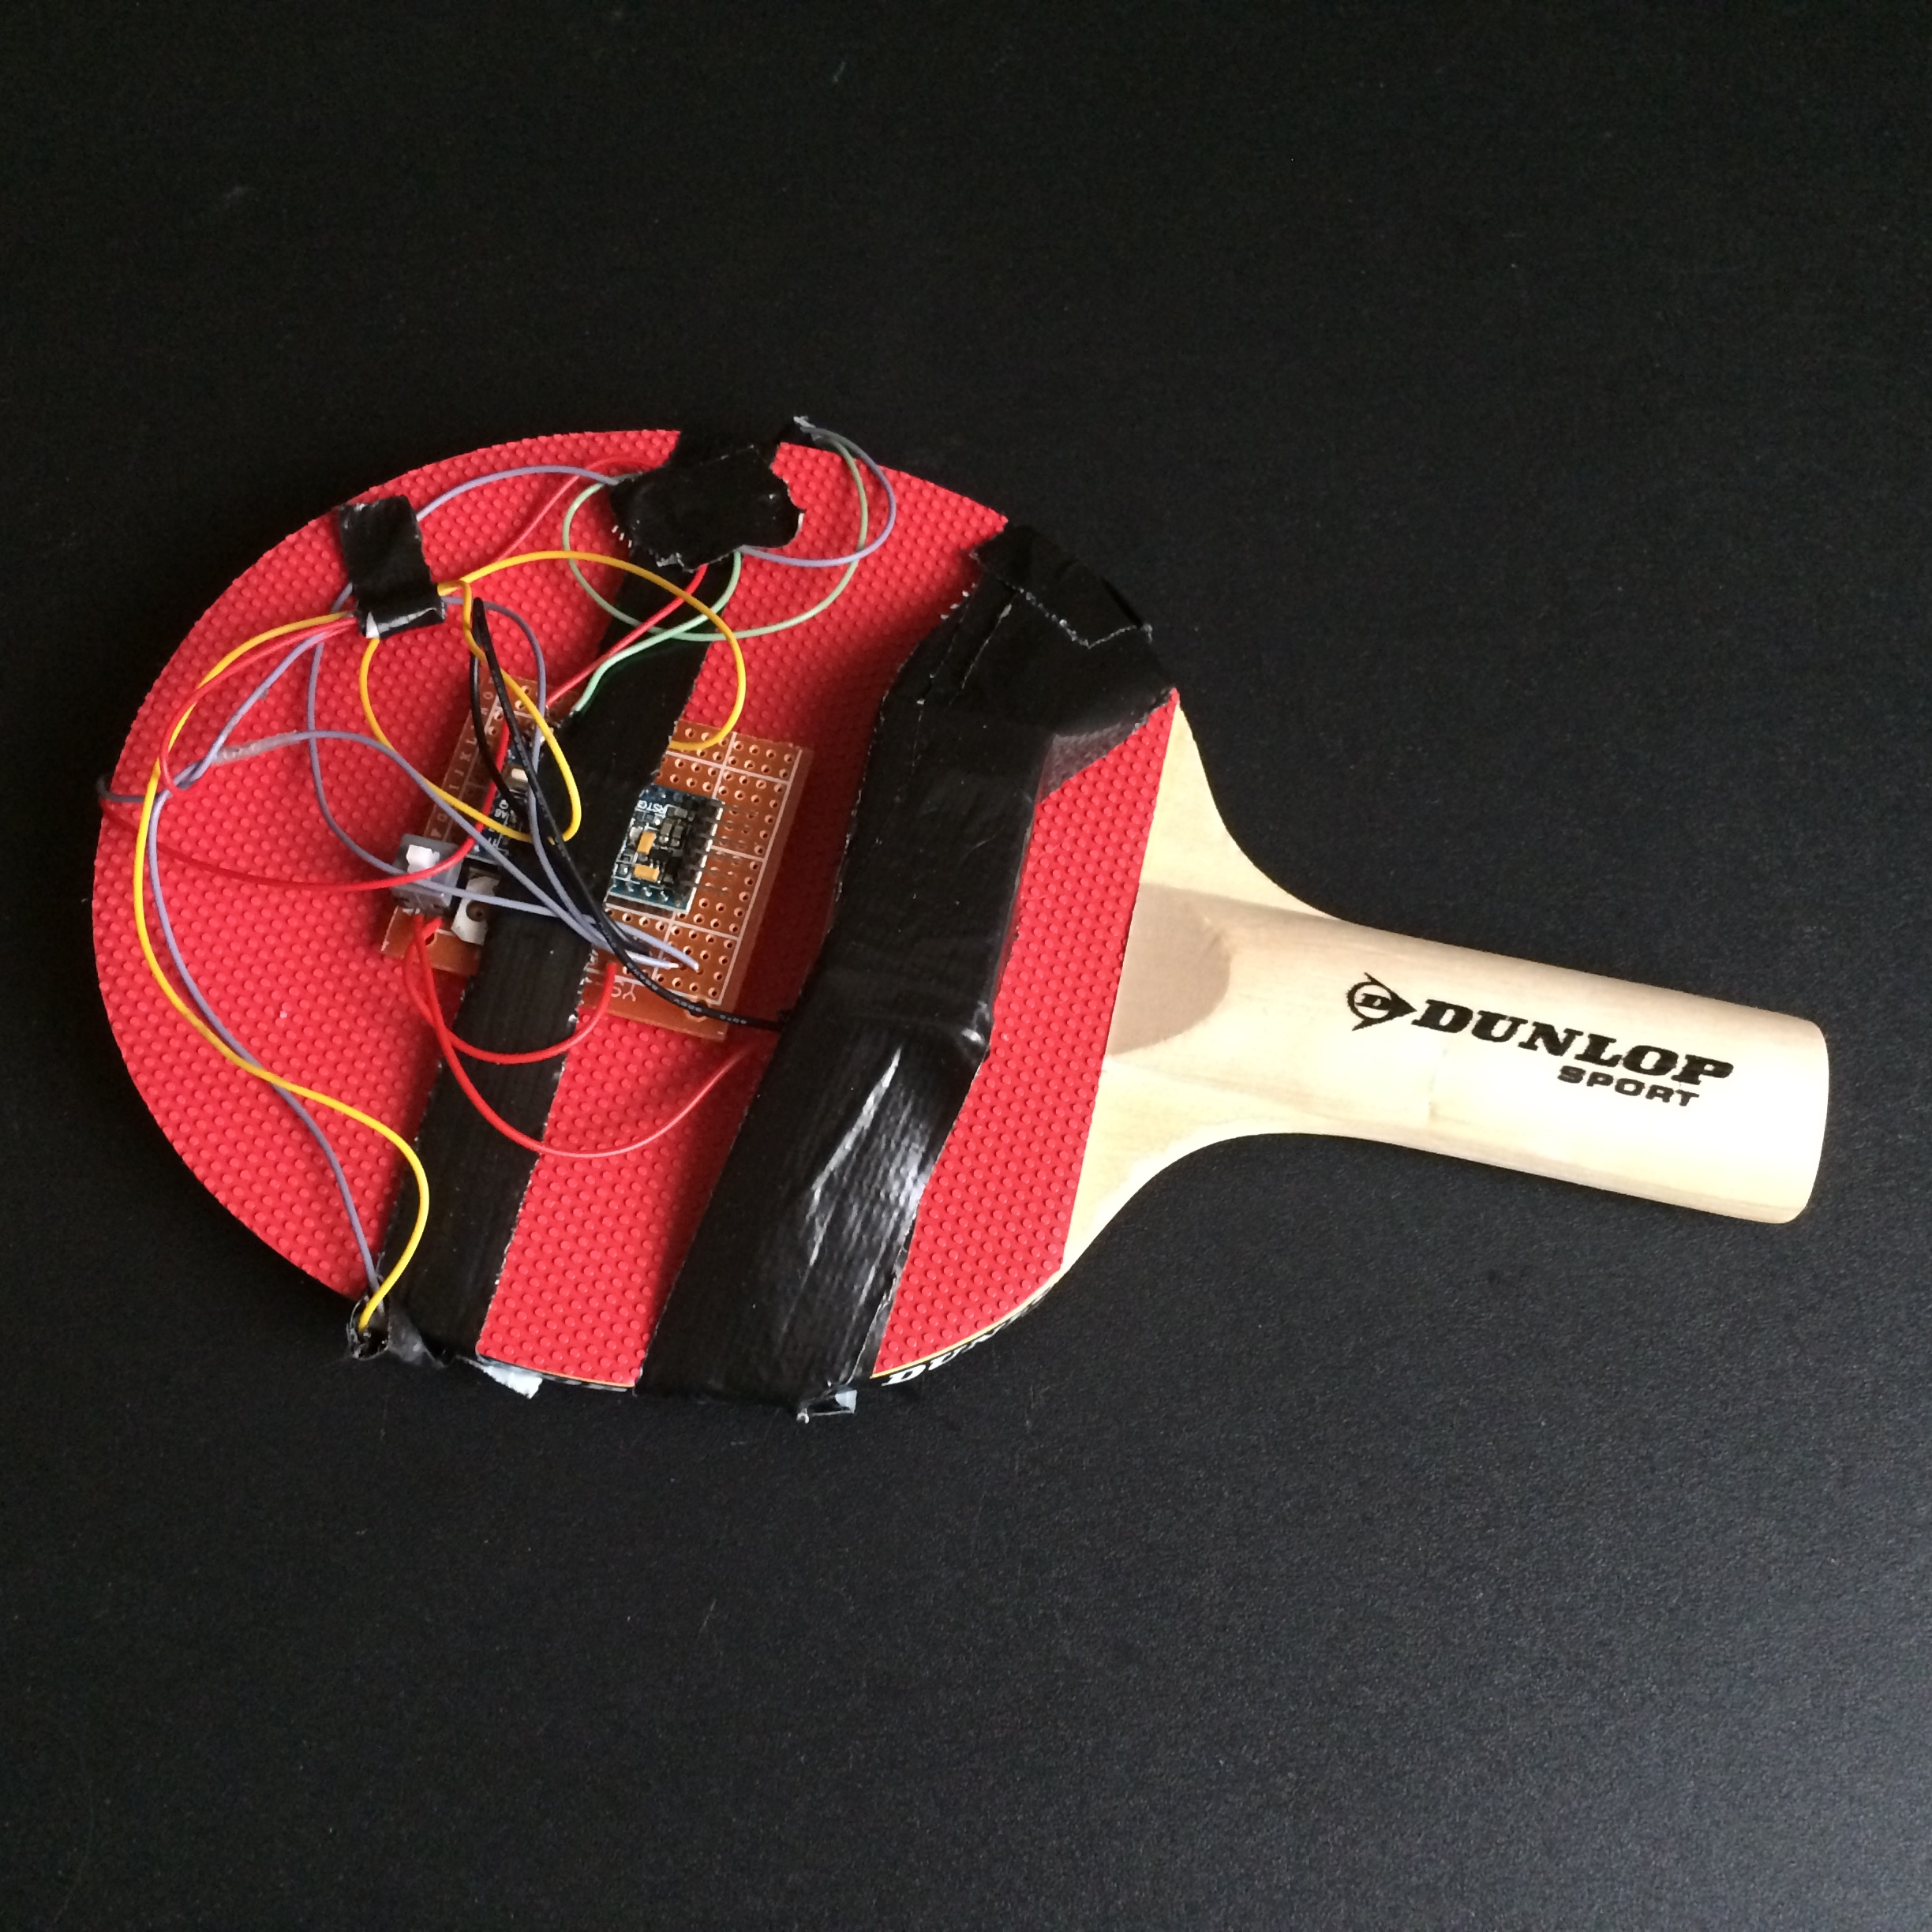
\includegraphics[width=0.6\columnwidth]{images/IMG_4364.JPG}
\begin{center}
\footnotesize{
\textit{\thecimages. attēls. Galda tenisa rakete aprīkota ar infrasarkanajiem gaismas marķieriem.}}
\end{center}
\end{center}
\end{samepage}

\refstepcounter{cimages}\label{cimages:pong_sample.png}
\vspace{10pt}
\begin{samepage}
\begin{center}
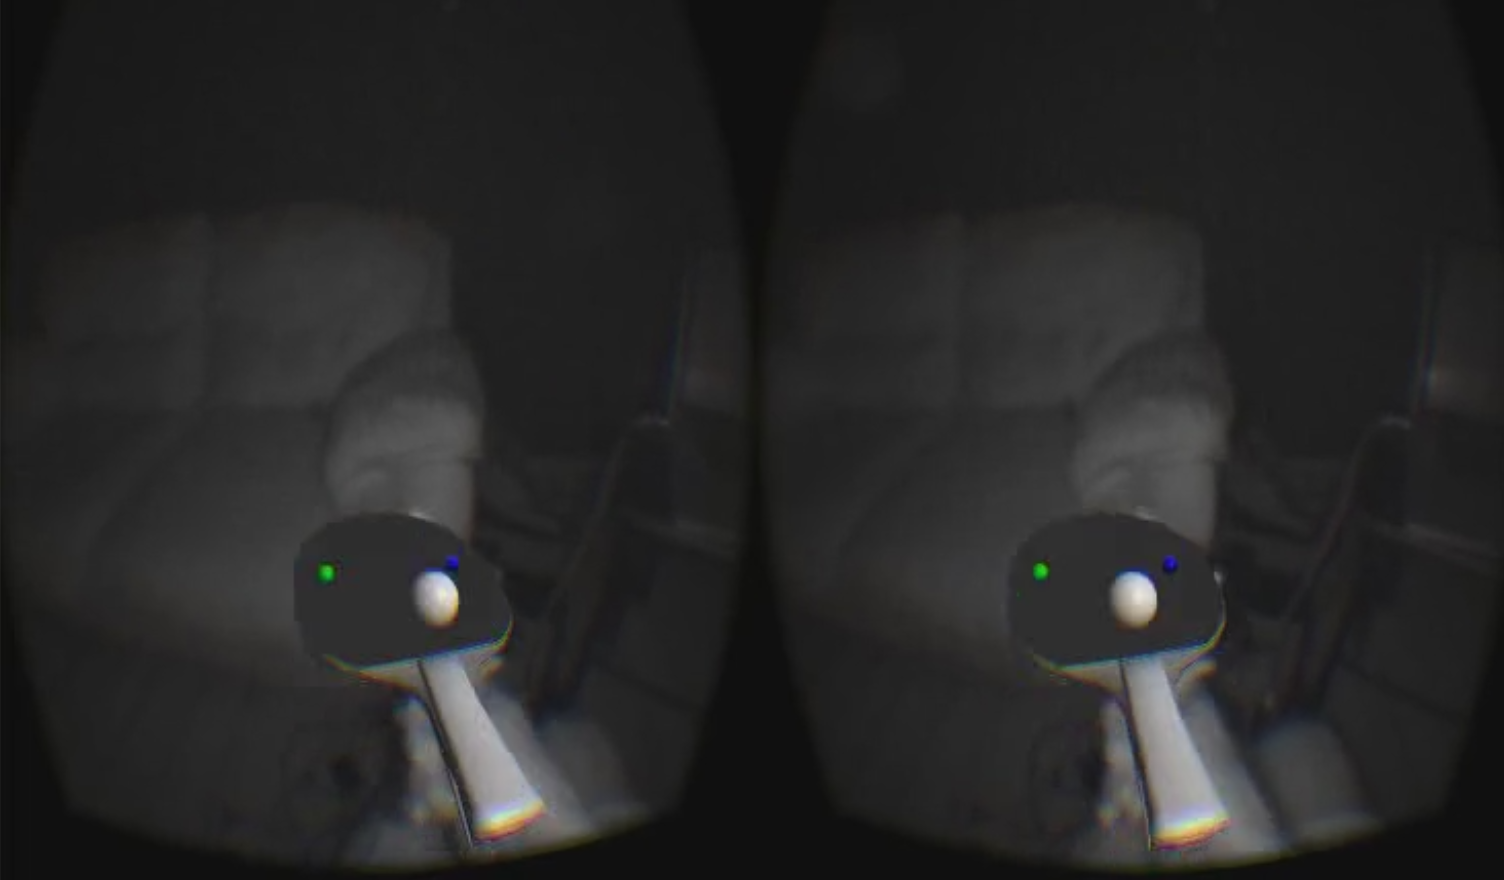
\includegraphics[width=0.6\columnwidth]{images/pong_sample.png}
\begin{center}
\footnotesize{
\textit{\thecimages. attēls. Galda tenisa raketes pozīcija iezīmēta paplašinātajā realitātē.}}
\end{center}
\end{center}
\end{samepage}

\newpage
\par
Viss šajā pētījumā izmantotais programmu primkods ir pieejams publiski pieejamā GIT repozitorijā
interneta vietnē:
\url{https://github.com/evaldsurtans/active-ir-markers}

\refstepcounter{cimages}\label{cimages:pong_raw_2.png}
\vspace{10pt}
\begin{samepage}
\begin{center}
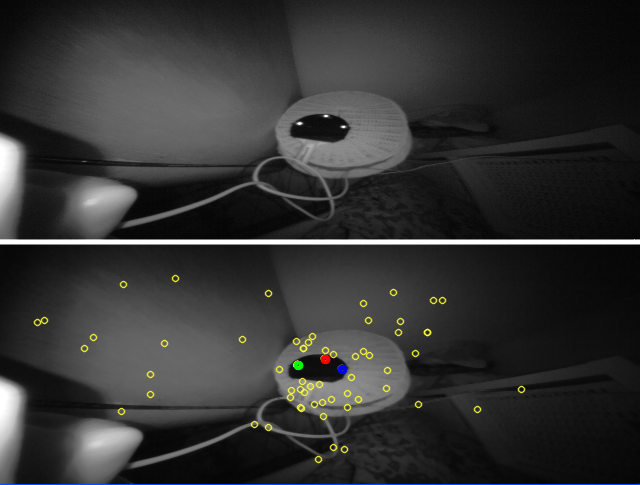
\includegraphics[width=0.9\columnwidth]{images/pong_new_1.png}
\begin{center}
\footnotesize{
\textit{\thecimages. attēls. Galda tenisa raketes pozīcija iezīmēta paplašinātajā realitātē.}}
\end{center}
\end{center}
\end{samepage}

\newpage
\subsection{Infrasarkano marķieru komunikācijas protokols}\label{section_protocol}

\par
Lai nodrošinātu marķieru identifikāciju, tika izveidots komunikācijas protokols, kas ir piemērots
datu pārraidei, izmantojot relatīvi zemas frekvences infrasarkano kameru. Šajā gadījumā datu 
nolasīšanai tika izmantotas Leap Motion infrasarkanās kameras ar 111 Hz frekvenci, kura nav stabila,
bet datu pārraide notika, mainot gaismas diodes intensitāti ar 37 Hz frekvenci.


\par
Datu pārraide notiek, izmantojot signāla kadrus, kur 3 signāla kadri paredzēti 1 bita pārraidei. Šāds
kadru sadalījums ļauj nolasītajos datos veikt ātru un efektīvu kļūdu apstrādi, izslēdzot neiespējamus
datu pārraides gadījumus. Šādu metodi nereti sauc arī par \textbf{FEC} algoritmu (\textit{Forward Error Correction}).

\begin{samepage}
\begin{table}[h]
\centering
\begin{tabular}{|l|l|l|}
\hline
\begin{tabular}[c]{@{}l@{}}Nolasītā kadru\\ vērtība\end{tabular} & \begin{tabular}[c]{@{}l@{}}Pārraidītā kadru\\ vērtība\end{tabular} & \begin{tabular}[c]{@{}l@{}}Datu bita\\ vērtība\end{tabular} \\ \hline
\cellcolor[HTML]{9AFF99}111                                      & 111                                                                & 1                                                           \\ \hline
\cellcolor[HTML]{9AFF99}000                                      & 000                                                                & 0                                                           \\ \hline
\cellcolor[HTML]{FFCCC9}001                                      & 000                                                                & 0                                                           \\ \hline
\cellcolor[HTML]{FFCCC9}010                                      & 000                                                                & 0                                                           \\ \hline
\cellcolor[HTML]{FFCCC9}100                                      & 000                                                                & 0                                                           \\ \hline
\cellcolor[HTML]{FFCCC9}110                                      & 111                                                                & 1                                                           \\ \hline
\cellcolor[HTML]{FFCCC9}101                                      & 111                                                                & 1                                                           \\ \hline
\cellcolor[HTML]{FFCCC9}011                                      & 111                                                                & 1                                                           \\ \hline
\end{tabular}
\end{table}
\vspace{-0.5cm}
\refstepcounter{ctables}\label{ctables:hamming_1}
\begin{center}
\footnotesize{
\textit{\thectables. tabula. Iespējamās kadru vērtības un to labojumi izmantojot, 3 kadrus viena bita vērtībai.}}
\end{center}
\end{samepage}


\par 
Datu nolasīšana ar kameras attēliem diemžēl nenotiek stabili ar 111 Hz frekvenci, taču ir iespējams
iegūt laika mērījumus starp katru iegūto attēlu. No šiem mērījumiem var aprēķināt, cik kadri ir izlaisti
laika posmā kopš pēdējā apskatītā kadra. Izlaisto kadru dati katram potenciālajam marķieru punktam 
tiek saglabāti kā biti ar nenoteiktu vērtību, kas var būt 1 vai 0 datu pēcapstrādē. 
Piemēram, nolasot datu signālu no kadriem, kuri ierodas ar 9 ms (111 Hz) laika nobīdi, var iegūt precīzu
informāciju par kadru vērtībām, taču regulāri kadri no kameras tiek iegūti ar dažādu laika nobīdi, kura
var būt 18ms, 20ms, utt. Šādos gadījumos tiek saglabāta īpaša bita vērtība "?", kura var vienlaicīgi būt
gan 1 vai 0 pēc nepieciešamības tālākajā datu apstrādē. Šādu vērtību visērtāk apstrādāt, ja tālākā atkļūdošanā
netiek izmantoti Haminga algoritmi, taču, izveidojot papildus kombināciju slāni, to var pielietot arī šajos
atkļūdošanas algoritmos. Šāda problēma ar nepastāvīgu laiku starp kadriem Leap Motion sensoram ir novērota arī citu pētnieku darbos \cite{JozeGuna2014}.

\begin{samepage}
\begin{table}[h]
\centering
\begin{tabular}{|l|l|l|l|l|l|l|l|}
\hline
Kadra laika nobīde & 9ms & 8ms & 9ms & \multicolumn{2}{l|}{18ms}     & 7ms & 9ms \\ \hline
Punkta vērtība     & 1   & 0   & 1   & 1 & \cellcolor[HTML]{FFCCC9}? & 1   & 0   \\ \hline
\end{tabular}
\end{table}
\vspace{-0.5cm}
\refstepcounter{ctables}\label{ctables:hamming_1}
\begin{center}
\footnotesize{
\textit{\thectables. tabula. Neregulāras kameras kadru frekvences labojuma bitu piemērs.}}
\end{center}
\end{samepage}

\par
Komunikācijas protokola izveidē tika apvienoti pētījumi par signālu apstrādi, kurus izmanto infrasarkanās
gaismas komunikācijā, izmantojot analogās shēmas, piemēram, televīzijas un citās bezvadu pultīs.
Iekārtu tālvadības pultīs, kas darbojas ar infrasarkano gaismu, pārsvarā izmanto 2 veidu fiziskā līmeņa protokolus \cite{ThibautRaharijaona2010}:
\begin{itemize}
\item Impulsa distances kodēšana, kur biti tiek iegūti mērot impulsa garumu laikā. Šādās shēmās nepieciešama laika
sinhronizācija, izmantojot sinhronizētus pulksteņus. Oculus Rift infrasarkanā kamera izmanto speciālu papildus
vadu no kameras līdz diodēm, lai panāktu šādu sinhronizāciju. Šāda metode nav piemērota, ja marķieri 
tiek iebūvēti ikdienas objektos, kuri nav savienoti ar vadiem, kā arī gadījumos, kad iebūvētajās shēmās
nav stabilas takts frekvences vai pulkstenis.
\item Mančestras kodēšana, kur biti tiek iegūti no signāla amplitūdas kāpuma un krituma bez laika sinhronizācijas.
Šīs kodēšanas princips ir līdzīgs Morzes kodam, kur eksistē tikai gari vai īsi signāli, nemērot laiku starp signāliem.
Atšķirībā no Morzes koda šī kodēšana nodrošina, ka netiek lieki aizņemts pārraides laiks un signāla amplitūdas 
mainās nepārtraukti ar vienādu frekvenci, bet pie bita maiņas maina tikai pārraides fāzi.
\end{itemize}


\par
Piedāvātais komunikācijas protokols darbojas vienā virzienā - datu pārraidei no \\ marķieriem uz infrasarkano
kameru. Lai vienkāršotu un nesadārdzinātu digitālo datu pārraides shēmu, mikrokontrolieris neizmanto precīzu pulksteņa mehānismu,
bet tikai takts frekvenci, kura nav pilnīgi stabila.
Tā kā datu pārraidei netiek izmantots stabils pulkstenis, tad visi pārraidītie dati tiek kodēti,
izmantojot Mančestras kodēšanas algoritmu, kas nodrošina datu pārraidi mainīga mikrokontroliera pulksteņa
gadījumā. Mančestras kodējumā katrs intensitātes jeb amplitūdas pieaugums tiek uzskatīts kā pilns bits
jeb 1, un katrs intensitātes kritums tiek uzskatīts kā tukšs bits jeb 0. Ja laika periods līdz
nākamai intensitātes izmaiņai ir mazāks par pusi no datu kadra ilguma, tad saglabājas iepriekšējā
bita vērtība \cite{ThibautRaharijaona2010}.

\refstepcounter{cimages}\label{cimages:ThibautRaharijaona2010_1.png}
\vspace{10pt}
\begin{samepage}
\begin{center}
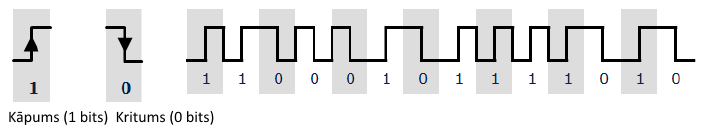
\includegraphics[width=0.8\columnwidth]{images/ThibautRaharijaona2010_1.png}
\begin{center}
\footnotesize{
\textit{\thecimages. attēls. Mančestras kodēšanas piemērs.}}
\end{center}
\end{center}
\end{samepage}

\refstepcounter{cimages}\label{cimages:machester_2.png}
\vspace{10pt}
\begin{samepage}
\begin{center}
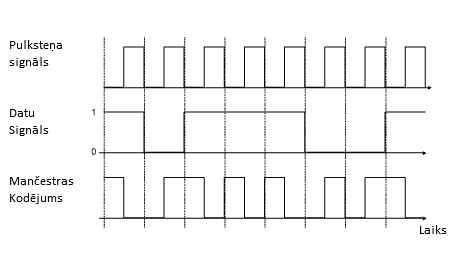
\includegraphics[width=0.8\columnwidth]{images/machester_2.png}
\begin{center}
\footnotesize{
\textit{\thecimages. attēls. Mančestras kodēšana, izmantojot pārraidītāja pulksteni.}}
\end{center}
\end{center}
\end{samepage}

Pirms katra skaitļa pārraides tiek pārraidīts signāls datu pārraides sākšanai. Piedāvātajā protokolā
tas ir 3 bitu ilgs zemas intensitātes signāls "0" un 1 bita augstas intensitātes signāls "1". Pārtraukuma signāls
nevar sastāvēt tikai no "0" vai "1", jo paši datu signāli var sākties un beigties ar "0" un "1". Vēl jāņem
vērā arī katra izvēlētā pārraidāmā identifikatora kodējums, jo, piemēram, Mančestras kodējumā ilgākais
signāls var būt 2 biti, tāpēc pārtraukuma signālam jābūt garākam par 2 bitiem. Gadījumā,
ja pārraidāmie dati vienmēr sākas vai beidzas ar "1", tad pārtraukuma signālā papildus bits nav nepieciešams, kā tas
parādīts \prettyref{ctables:idc_1}.tabulā. Gadījumos, kad identifikācijas kodi virknē nepārklājas, ir iespējams
vispār nepārraidīt pārtraukuma kodu. Šāda implementācija nebūs universāli izmantojama, taču kontrolētā
vidē tā var būt noderīga, lai samazinātu pārraidāmo datu apjomu.

\begin{samepage}
\begin{table}[h]
\centering
\begin{tabular}{|l|l|}
\hline
\rowcolor[HTML]{D0D0D0} 
Identifikācijas kods & Apraksts                         \\ \hline
10100                & 1. marķiera identifikācijas kods \\ \hline
10101                & 2. marķiera identifikācijas kods \\ \hline
11100                & 3. marķiera identifikācijas kods \\ \hline
000                  & Pārtraukuma kods                 \\ \hline
\end{tabular}
\end{table}
\begin{table}[h]
\centering
\begin{tabular}{|l|l|l|l|l|
>{\columncolor[HTML]{9AFF99}}l |
>{\columncolor[HTML]{9AFF99}}l |
>{\columncolor[HTML]{9AFF99}}l |
>{\columncolor[HTML]{9AFF99}}l |
>{\columncolor[HTML]{9AFF99}}l |l|l|l|l|l|l|l|l|l|l|}
\hline
1 & 0 & 1 & 0 & 0 & 1 & 0 & 1 & 0 & 0 & 1 & 0 & 1 & 0 & 0 & 1 & 0 & 1 & 0 & 0 \\ \hline
1 & 0 & 1 & 0 & 1 & 1 & 0 & 1 & 0 & 1 & 1 & 0 & 1 & 0 & 1 & 1 & 0 & 1 & 0 & 1 \\ \hline
1 & 1 & 1 & 0 & 0 & 1 & 1 & 1 & 0 & 0 & 1 & 1 & 1 & 0 & 0 & 1 & 1 & 1 & 0 & 0 \\ \hline
\end{tabular}
\end{table}
\begin{table}[h]
\centering
\begin{tabular}{|l|l|l|l|l|
>{\columncolor[HTML]{CBCEFB}}l |
>{\columncolor[HTML]{CBCEFB}}l |
>{\columncolor[HTML]{CBCEFB}}l |
>{\columncolor[HTML]{9AFF99}}l |
>{\columncolor[HTML]{9AFF99}}l |
>{\columncolor[HTML]{9AFF99}}l |
>{\columncolor[HTML]{9AFF99}}l |
>{\columncolor[HTML]{9AFF99}}l |
>{\columncolor[HTML]{CBCEFB}}l |
>{\columncolor[HTML]{CBCEFB}}l |
>{\columncolor[HTML]{CBCEFB}}l |
>{\columncolor[HTML]{FFFFFF}}l |
>{\columncolor[HTML]{FFFFFF}}l |
>{\columncolor[HTML]{FFFFFF}}l |l|}
\hline
1 & 0 & 1 & 0 & 0 & 0 & 0 & 0 & 1 & 0 & 1 & 0 & 0 & 0 & 0 & 0 & 1 & 0 & 1 & 0 \\ \hline
1 & 0 & 1 & 0 & 1 & 0 & 0 & 0 & 1 & 0 & 1 & 0 & 1 & 0 & 0 & 0 & 1 & 0 & 1 & 0 \\ \hline
1 & 1 & 1 & 0 & 0 & 0 & 0 & 0 & 1 & 1 & 1 & 0 & 0 & 0 & 0 & 0 & 1 & 1 & 1 & 0 \\ \hline
\end{tabular}
\end{table}
\vspace{-0.5cm}
\refstepcounter{ctables}\label{ctables:idc_1}
\begin{center}
\footnotesize{
\textit{\thectables. tabula. Marķieru identifikācijas kodi un pārtraukuma kods. Piemēri pārraidot datus virknē bez pārtraukuma koda, un, izmantojot pārtraukuma kodu.}}
\end{center}
\end{samepage}

\newpage

\begin{samepage}
\begin{table}[h]
\centering
\begin{tabular}{|l|l|}
\hline
\rowcolor[HTML]{D0D0D0} 
Identifikācijas kods & Apraksts                         \\ \hline
00110                & 1. marķiera identifikācijas kods \\ \hline
10101                & 2. marķiera identifikācijas kods \\ \hline
11100                & 3. marķiera identifikācijas kods \\ \hline
000                  & Pārtraukuma kods                 \\ \hline
\end{tabular}
\end{table}
\vspace{-0.5cm}
\refstepcounter{ctables}\label{ctables:idc_1}
\begin{center}
\footnotesize{
\textit{\thectables. tabula. Marķieru identifikācijas kodi un pārtraukuma kods gadījumā, kad pārraidāmie dati nav noteikti.}}
\end{center}
\end{samepage}


\begin{samepage}
\begin{table}[h]
\centering
\begin{tabular}{|l|l|l|l|l|
>{\columncolor[HTML]{CBCEFB}}l |
>{\columncolor[HTML]{CBCEFB}}l |
>{\columncolor[HTML]{CBCEFB}}l |
>{\columncolor[HTML]{9AFF99}}l |
>{\columncolor[HTML]{9AFF99}}l |
>{\columncolor[HTML]{9AFF99}}l |
>{\columncolor[HTML]{9AFF99}}l |
>{\columncolor[HTML]{9AFF99}}l |
>{\columncolor[HTML]{CBCEFB}}l |
>{\columncolor[HTML]{CBCEFB}}l |
>{\columncolor[HTML]{CBCEFB}}l |
>{\columncolor[HTML]{FFFFFF}}l |
>{\columncolor[HTML]{FFFFFF}}l |
>{\columncolor[HTML]{FFFFFF}}l |l|}
\hline
0 & 0 & 1 & 0 & \cellcolor[HTML]{FFFFFF}0 & \cellcolor[HTML]{FFFFFF}0 & \cellcolor[HTML]{FFFFFF}0 & \cellcolor[HTML]{FFCCC9}0 & \cellcolor[HTML]{FFCCC9}0 & \cellcolor[HTML]{FFCCC9}0 & 1 & 0 & 0 & \cellcolor[HTML]{9AFF99}0 & \cellcolor[HTML]{9AFF99}0 & \cellcolor[HTML]{FFCCC9}0 & \cellcolor[HTML]{FFCCC9}0 & \cellcolor[HTML]{FFCCC9}0 & 1 & 0 \\ \hline
1 & 0 & 1 & 0 & 1                         & 0                         & 0                         & 0                         & 1                         & 0                         & 1 & 0 & 1 & 0                         & 0                         & 0                         & 1                         & 0                         & 1 & 0 \\ \hline
1 & 1 & 1 & 0 & 0                         & 0                         & 0                         & 0                         & 1                         & 1                         & 1 & 0 & 0 & 0                         & 0                         & 0                         & 1                         & 1                         & 1 & 0 \\ \hline
\end{tabular}
\end{table}
\vspace{-0.5cm}
\refstepcounter{ctables}\label{ctables:idc_1}
\begin{center}
\footnotesize{
\textit{\thectables. tabula. Ja tiek izmantots pārtraukuma kods "000", tad rodas kļūda 1. marķiera datu pārraidē, jo pārtraukuma kods pārklājas ar pārraidāmo datu iespējamajiem kodiem.}}
\end{center}
\end{samepage}

\begin{samepage}
\begin{table}[h]
\centering
\begin{tabular}{|l|l|l|l|l|
>{\columncolor[HTML]{CBCEFB}}l |
>{\columncolor[HTML]{CBCEFB}}l |
>{\columncolor[HTML]{CBCEFB}}l |
>{\columncolor[HTML]{CBCEFB}}l |
>{\columncolor[HTML]{9AFF99}}l |
>{\columncolor[HTML]{9AFF99}}l |
>{\columncolor[HTML]{9AFF99}}l |
>{\columncolor[HTML]{9AFF99}}l |
>{\columncolor[HTML]{9AFF99}}l |
>{\columncolor[HTML]{CBCEFB}}l |
>{\columncolor[HTML]{CBCEFB}}l |
>{\columncolor[HTML]{CBCEFB}}l |
>{\columncolor[HTML]{CBCEFB}}l |
>{\columncolor[HTML]{FFFFFF}}l |
>{\columncolor[HTML]{FFFFFF}}l |
>{\columncolor[HTML]{FFFFFF}}l |}
\hline
0 & 0 & 1 & 0 & \cellcolor[HTML]{FFFFFF}0 & 0 & 0 & 0 & 1 & 0 & 0 & 1 & 0 & 0 & 0 & 0 & 0 & 1 & 0 & 0 & 1 \\ \hline
1 & 0 & 1 & 0 & 1                         & 0 & 0 & 0 & 1 & 1 & 0 & 1 & 0 & 1 & 0 & 0 & 0 & 1 & 1 & 0 & 1 \\ \hline
1 & 1 & 1 & 0 & 0                         & 0 & 0 & 0 & 1 & 1 & 1 & 1 & 0 & 0 & 0 & 0 & 0 & 1 & 1 & 1 & 1 \\ \hline
\end{tabular}
\end{table}
\vspace{-0.5cm}
\refstepcounter{ctables}\label{ctables:idc_1}
\begin{center}
\footnotesize{
\textit{\thectables. tabula. Pareizi izvēlēts pārtraukuma signāla kods, lai varētu apstrādāt jebkādus datus, kuru bitu virknes nesastāv no vairāk nekā 2 vienādiem blakusesošiem bitiem, piemēram, Mančestras kodējumā.}}
\end{center}
\end{samepage}

\par 
Nodrošinot datu posma slāni, sūtītie dati tiek kodēti, izmantojot pāra bita algoritmu (\textit{parity bit}), kas nodrošina datu kļūdas labojumu,
ja kļūda ir konstatēta vienā no pārraidītā ciparu signāla bitiem. Šis kodējums tiek pielietots
pārraidāmajiem datiem pirms Mančestras kodējuma.
Pāra bitu algoritmā starp pārraidāmajiem bitiem katrā bita vietā, kura indekss ir $2^k$ pakāpe tiek
ievietots papildus bits, kurš tiek aprēķināts pēc sekojoša algoritma. Katra atkļūdošanas bita indekss $k$
norāda uz šī bita aprēķina virknes skaitļiem jeb bitiem. Piemēram, ja $k = 1$, tad, aprēķinot pārbaudes bitu, 
pozīcijā $b_1$ tiek ņemts vērā pirmais bits, tad tiek viens izlaists, tad atkal tiek saglabāts viens bits, tad
atkal tiek viens izlaists. Tā tiek saglabāti visi biti līdz rindas beigām. Ja $k = 2$ tad tiek saglabāti pirmie 2 biti,
tad 2 tiek izlaisti, tad atkal 2 tiek saglabāti. Tā atkal tiek saglabāta bitu virkne $b_2$ līdz rindas beigām.
Katra bitu virkne tiek saglabāta sākot ar $k$ bita indeksu no aprēķināma $b_k$ bita. Ja ir sasniegtas bitu virknes beigas,
tad vairāk biti netiek saglabāti virknē. Piemēram, 8 bitu virknē $b_4$ un $b_8$ būs tikai 4 bitu gara virkne. 
Kad ir iegūtas atkļūdošanas bitu virknes, tad iegūtie biti tiek saskaitīti decimālajā sistēmā, un, ja
summa ir pāra skaitlis, tad bita vērtība tiek piešķirta kā 0, bet ja tā ir nepāra skaitlis, tad bita vērtība
tiek piešķirta kā vērtība "1".
\newpage
\par 
Piemērā ir dots pāru bitu algoritma pielietojums 8 bitu datu pārraidei. Pārraidāmā
datu virkne ir $D$, kas satur bitu vērtības, datu virkne ar pāru bitu atkļūdošanas bitiem ir $D'$,
bet $b_1$, $b_2$, $b_4$, $b_8$ ir pāru jeb atkļūdošanas biti.
$$
D = \{0,1,0,0,1,1,0,1\} \\
$$
$$
D' = \{b_1,b_2,0,b_4,1,0,0,b_8,1,1,0,1\} = \{0,1,0,0,1,0,0,1,1,1,0,1\} 
$$
$$
b_1 \rightarrow \{b_1,0,1,0,1,0\} \rightarrow 0 + 1 + 0 + 1 + 0 = 2 \rightarrow 2\ MOD\ 2 = 0
$$
$$
b_2 \rightarrow \{b_2,0,0,0,1,0\} \rightarrow 0 + 0 + 0 + 1 + 0 = 1 \rightarrow 1\ MOD\ 2 = 1
$$
$$
b_4 \rightarrow \{b_4,1,0,0,1\} \rightarrow 1 + 0 + 0 + 1 = 2 \rightarrow 2\ MOD\ 2 = 0
$$
$$
b_8 \rightarrow \{b_8,1,1,0,1\} \rightarrow 1 + 1 + 0 + 1 = 3 \rightarrow 3\ MOD\ 2 = 1
$$

\par
Pēc datu saņemšanas pāru bitu tiek pārbaudīti un ir iespējams izlabot viena bita kļūdu, neizmantojot nekādu
papildus informāciju, kā tikai pāru bitu vērtības. Vispirms tiek saglabātas pāru bitu vērtības
tieši tāpat kā pirms sūtīšanas, pēc tam tiek salīdzinātas $b_k$ vērtības ar aprēķinātajām, un 
visbeidzot, visu kļūdaino $b_k$ bitu pakāpju vērtības $k$ tiek saskaitītas. Iegūtā summa norāda uz kļūdaino
bitu, kurš jāmaina uz pretējo vērtību.

\par 
Pāru bitu algoritma atkļūdošanas piemērs dots sekojošā aprēķinā, kur $D''$ ir saņemtā bitu
virkne ar kļūdu, bet $D'$ ir iepriekš aprēķinātā bitu virkne bez kļūdas.
$$
D'' = \{0,1,0,0,1,0,0,1,1,1,1,1\} 
$$
$$
b_1 = 1 \rightarrow \{b_1,0,1,0,1,1\} \rightarrow 0 + 1 + 0 + 1 + 1 = 3 \rightarrow 3\ MOD\ 2 \neq 0
$$
$$
b_2 = 1 \rightarrow \{b_2,0,0,0,1,1\} \rightarrow 0 + 0 + 0 + 1 + 1 = 2 \rightarrow 2\ MOD\ 2 \neq 1
$$
$$
b_4 = 0 \rightarrow \{b_4,1,0,0,1\} \rightarrow 1 + 0 + 0 + 1 = 2 \rightarrow 2\ MOD\ 2 = 0
$$
$$
b_8 = 1 \rightarrow \{b_8,1,1,1,1\} \rightarrow 1 + 1 + 1 + 1 = 4 \rightarrow 4\ MOD\ 2 \neq 1
$$
Kļūdas ir $b_1$, $b_2$ un $b_8$ bitos, kuriem nepieciešams saskaitīt pakāpju vērtības.
$$
s = 1 + 2 + 8 = 11
$$
Iegūtā vērtība $s$ norāda uz bitu, kurš ir kļūdains. Kā redzams, nomainot $D''$ kļūdainās virknes 11 bitu uz
pretējo vērtību tā sakrīt ar sākotnējo $D'$ bitu virkni.
Lai iegūtu sākotnējo datu virkni nepieciešams vienkārši izņemt pāru bitus no $D'$ virknes.

\newpage
\par
Haminga kodējuma algoritmu parasti implementē, izmantojot "izslēdzošo vai" operatoru (XOR).
Izmantojot iepriekšējā piemērā doto bitu virkni, algoritma izpildāmie soļi ir sekojošie \cite{HenryS.Warren2012}:
$$
D = \{0,1,0,0,1,1,0,1\} 
$$

\begin{samepage}
\vspace{-0.5cm}
\begin{table}[h]
\centering
\begin{tabular}{|l|l|l|l|l|l|l|l|l|l|l|l|}
\hline
1 & 2 & 3 & 4 & \cellcolor[HTML]{77FF77}5 & 6 & 7 & 8 & \cellcolor[HTML]{77FF77}9 & \cellcolor[HTML]{77FF77}10 & 11 & \cellcolor[HTML]{77FF77}12 \\ \hline
\cellcolor[HTML]{FFFFC7}$b_1$  & \cellcolor[HTML]{FFFFC7}$b_2$  & 0 & \cellcolor[HTML]{FFFFC7}$b_4$  & \cellcolor[HTML]{77FF77}1 & 0 & 0 & \cellcolor[HTML]{FFFFC7}$b_8$  & \cellcolor[HTML]{77FF77}1 & \cellcolor[HTML]{77FF77}1  & 0  & \cellcolor[HTML]{77FF77}1  \\ \hline
\end{tabular}
\end{table}
\vspace{-0.5cm}
\refstepcounter{ctables}\label{ctables:hamming_1}
\begin{center}
\footnotesize{
\textit{\thectables. tabula. Bitu virkne ar indeksiem un pāru bitiem $b_k$.}}
\end{center}
\end{samepage}

\begin{samepage}
\begin{table}[h]
\centering
\begin{tabular}{|l|l|l|l|l|}
\hline
\rowcolor[HTML]{FFFFC7} 
\begin{tabular}[c]{@{}l@{}}Bitu indeksi\\ ar vērtībām "1"\end{tabular}                                                & $b_8$       & $b_4$       & $b_2$       & $b_1$       \\ \hline
\cellcolor[HTML]{77FF77}\begin{tabular}[c]{@{}l@{}}5 (decimālais skaitlis) = \\ 0101 (binārais skaitlis)\end{tabular} & 0          & 1          & 0          & 1          \\ \hline
\cellcolor[HTML]{77FF77}9 = 1001                                                                                      & 1          & 0          & 0          & 1          \\ \hline
\cellcolor[HTML]{77FF77}10 = 1010                                                                                     & 1          & 0          & 1          & 0          \\ \hline
\cellcolor[HTML]{77FF77}12 = 1100                                                                                     & 1          & 1          & 0          & 0          \\ \hline
\rowcolor[HTML]{EFEFEF} 
\cellcolor[HTML]{EFEFEF}\begin{tabular}[c]{@{}l@{}}$b_k$ vērtība veicot XOR\\ starp vērtībām\end{tabular}              & \textbf{1} & \textbf{0} & \textbf{1} & \textbf{0} \\ \hline
\end{tabular}
\end{table}
\vspace{-0.5cm}
\refstepcounter{ctables}\label{ctables:hamming_1}
\begin{center}
\footnotesize{
\textit{\thectables. tabula. No bitu virknes, izmantojot XOR operatoru apvienot bitus, kas atbilst indeksu skaitļiem, pie kuriem virknē $D'$ vērtības ir "1" jeb pilns bits.}}
\end{center}
\end{samepage}


Iegūtais $D'$ sakrīt ar iepriekš apskatītajā piemērā iegūto ciparu virkni, izmantojot decimālo skaitīšanu.

$$
D' = \{0,1,0,0,1,0,0,1,1,1,0,1\} 
$$

\begin{samepage}
\vspace{-0.5cm}
\begin{table}[h]
\centering
\begin{tabular}{|l|l|l|l|l|l|l|l|l|l|l|l|}
\hline
1 & 2 & 3 & 4 & 5 & 6 & 7 & 8 & 9 & 10 & 11 & 12 \\ \hline
\cellcolor[HTML]{FFFFC7}0 & \cellcolor[HTML]{FFFFC7}1 & 0 & \cellcolor[HTML]{FFFFC7}0 & 1 & 0 & 0 & \cellcolor[HTML]{FFFFC7}1 & 1 & 1  & 0  & 1  \\ \hline
\end{tabular}
\end{table}
\vspace{-0.5cm}
\refstepcounter{ctables}\label{ctables:hamming_1}
\begin{center}
\footnotesize{
\textit{\thectables. tabula. Iegūtā bitu virkne $D'$ ar Hamminga kodējumu.}}
\end{center}
\end{samepage}

Lai paskaidrotu datu atkļūdošanu, izmantosim iepriekš apskatīto kļūdaino virkni $D''$, kur kļūdains ir 11 bits.

$$
D'' = \{0,1,0,0,1,0,0,1,1,1,1,1\} 
$$

\newpage
\begin{samepage}
\begin{table}[h]
\centering
\begin{tabular}{|l|l|l|l|l|l|l|l|l|l|l|l|}
\hline
1 & 2 & 3 & 4 & 5 & 6 & 7 & 8 & 9 & 10 & 11 & 12 \\ \hline
\cellcolor[HTML]{FFFFC7}0 & \cellcolor[HTML]{FFFFC7}1 & 0 & \cellcolor[HTML]{FFFFC7}0 & 1 & 0 & 0 & \cellcolor[HTML]{FFFFC7}1 & 1 & 1  & \cellcolor[HTML]{FFCCC9}1  & 1  \\ \hline
\end{tabular}
\end{table}
\vspace{-0.5cm}
\refstepcounter{ctables}\label{ctables:hamming_1}
\begin{center}
\footnotesize{
\textit{\thectables. tabula. Kļūdainā virkne $D''$ (11. bitā kļūda).}}
\end{center}
\end{samepage}

\begin{samepage}
\begin{table}[h]
\centering
\begin{tabular}{|l|l|l|l|l|}
\hline
\rowcolor[HTML]{FFFFC7} 
                                                                                           & $b_8$         & $b_4$         & $b_2$         & $b_1$         \\ \hline
\cellcolor[HTML]{FFFFC7}Saņemtie pāru biti                                                 & 1          & 0          & 1          & 0          \\ \hline
\cellcolor[HTML]{FFFFC7}Aprēķinātie pāru biti                                              & 0          & 0          & 0          & 1          \\ \hline
\rowcolor[HTML]{EFEFEF} 
\begin{tabular}[c]{@{}l@{}}Sindroma vērtība\\ (XOR)\end{tabular}                           & \textbf{1} & \textbf{0} & \textbf{1} & \textbf{1} \\ \hline
Sindroma vērtība                                                                            & \multicolumn{4}{l|}{11}                            \\ \hline
\begin{tabular}[c]{@{}l@{}}Kļūdainā bita indekss\end{tabular} & \multicolumn{4}{l|}{11}                  \\ \hline
\end{tabular}
\end{table}
\refstepcounter{ctables}\label{ctables:hamming_1}
\begin{center}
\footnotesize{
\textit{\thectables. tabula. Sindroma vērtības un kļūdainā bita indekss.}}
\end{center}
\end{samepage}

Hamminga kodējumā atkļūdošanas XOR rezultātu sauc par sindromu, kurš norāda uz kļūdaino bitu.
Šo algoritmu nereti sauc arī par SEC (\textit{single error correcting}) Hamminga algoritmu.

\par
Vēl sūtītajiem datiem tiek pievienots papildus bits, lai varētu veikt arī divu kļūdainu bitu labošanu,
izmantojot paplašināto Haminga attāluma algoritmu (\textit{Extended Hamming distance}).
Šo algoritmu nereti sauc arī par SEC-DEC (\textit{double error detecting}) Hamminga algoritmu.

Lai novērstu 2 bitu kļūdu, nepieciešams pievienot papildus bitu, kas ir visu pārējo bitu XOR kopējā vērtība \cite{HenryS.Warren2012}.
Papildus pārbaudes bita vērtība $b_{13}$ aprēķināta dotajā piemērā no sākotnējās virknes ar pāru bitiem $D'$.

\begin{equation}\label{eq:eq_1}
b_{13} = 0 \oplus 1 \oplus 0 \oplus 0 \oplus 1 \oplus 0 \oplus 0 \oplus 1 \oplus 1 \oplus 1 \oplus 0 \oplus 1 = 0
\end{equation}

$$
E' = \{0,1,0,0,1,0,0,1,1,1,0,1,0\} 
$$
\begin{samepage}
\begin{table}[h]
\centering
\begin{tabular}{|l|l|l|l|l|l|l|l|l|l|l|l|l|}
\hline
1                         & 2                         & 3 & 4                         & 5 & 6 & 7 & 8                         & 9 & 10 & 11 & 12 & 13                        \\ \hline
\cellcolor[HTML]{FFFFC7}0 & \cellcolor[HTML]{FFFFC7}1 & 0 & \cellcolor[HTML]{FFFFC7}0 & 1 & 0 & 0 & \cellcolor[HTML]{FFFFC7}1 & 1 & 1  & 0  & 1  & \cellcolor[HTML]{ECF4FF}0 \\ \hline
\end{tabular}
\end{table}
\refstepcounter{ctables}\label{ctables:hamming_1}
\begin{center}
\footnotesize{
\textit{\thectables. tabula. Iegūtā virkne ar pareiziem pāru bitiem $E'$.}}
\end{center}
\end{samepage}

\newpage
Papildinot iepriekšējo piemēru $D''$ zemāk dota virkne $E''$ ar 2 kļūdām.

$$
E'' = \{0,0,0,0,1,0,0,1,1,1,1,1,0\} 
$$

\begin{samepage}
\begin{table}[h]
\centering
\begin{tabular}{|l|l|l|l|l|l|l|l|l|l|l|l|l|}
\hline
1                         & 2                         & 3 & 4                         & 5 & 6 & 7 & 8                         & 9 & 10 & 11                        & 12 & 13                        \\ \hline
\cellcolor[HTML]{FFFFC7}0 & \cellcolor[HTML]{FFCCC9}0 & 0 & \cellcolor[HTML]{FFFFC7}0 & 1 & 0 & 0 & \cellcolor[HTML]{FFFFC7}1 & 1 & 1  & \cellcolor[HTML]{FFCCC9}1 & 1  & \cellcolor[HTML]{ECF4FF}0 \\ \hline
\end{tabular}
\end{table}
\refstepcounter{ctables}\label{ctables:hamming_1}
\begin{center}
\footnotesize{
\textit{\thectables. tabula. Virkne $E''$ ar 2 kļūdām. Viena no kļūdām ir pirmā līmeņa 2. pāra bitā.}}
\end{center}
\end{samepage}

Lai atkļūdotu doto virkni, tiek pielietota sekojoša likumu kopa.

\begin{samepage}
\begin{table}[h]
\centering
\begin{tabular}{|l|l|l|l|}
\hline
\multicolumn{2}{|l|}{Likumi}                                                                                                     & \multicolumn{2}{l|}{Secinājumi}                                                                                                                                                                  \\ \hline
\begin{tabular}[c]{@{}l@{}}Vai papildus\\ bits sakrīt?\end{tabular} & \begin{tabular}[c]{@{}l@{}}Sindroma\\ vērtība\end{tabular} & Kļūdu skaits & Apraksts                                                                                                                                                                          \\ \hline
$b_{13}'' = b_{13}'$                                                & 0                                                          & 0            & Nav kļūdu                                                                                                                                                                         \\ \hline
$b_{13}'' \neq b_{13}'$                                             & 0                                                          & 1            & Kļūda ir $b_{13}$ bitā                                                                                                                                                              \\ \hline
$b_{13}'' \neq b_{13}'$                                             & $\neq 0$                                                   & 1            & Sindroma vērtība norāda uz kļūdu                                                                                                                                                  \\ \hline
$b_{13}'' = b_{13}'$                                                & $\neq 0$                                                   & 2            & \begin{tabular}[c]{@{}l@{}}Nepieciešams pārbaudīt visas iespējamās\\ kombinācijas mainot SEC bitu pusē k=1..12\\ mainot pa vienam bitam un pārbaudot dotos\\ likumus\end{tabular} \\ \hline
\end{tabular}
\end{table}
\refstepcounter{ctables}\label{ctables:hamming_1}
\begin{center}
\footnotesize{
\textit{\thectables. tabula. Likumu kopa 2 bitu atkļūdošanai 8 bitu datu pārraidei.}}
\end{center}
\end{samepage}

\par
Dotajā piemērā pirmajā iterācijā tiks noskaidrots, ka $E''$ satur 2 kļūdas. Otrajā iterācijā
$b_1$ vērtība tiks nomainīta uz 1, un, atkārtojot likuma kopu, tiks noteikts, ka vēl joprojām ir vismaz 2
kļūdas. Pēc tam $b_2$ vērtība tiks nomainīta uz 1 un tiks noskaidrots, ka ir tikai viena kļūda,
kura atrodas 11. bitā, izmantojot sindroma vērtību.

\begin{samepage}
\begin{table}[h]
\centering
\begin{tabular}{|l|l|l|l|l|l|l|l|l|l|l|l|l|}
\hline
1                         & 2                         & 3 & 4                         & 5 & 6 & 7 & 8                         & 9 & 10 & 11                        & 12 & 13                        \\ \hline
\cellcolor[HTML]{9AFF99}1 & \cellcolor[HTML]{9AFF99}0 & 0 & \cellcolor[HTML]{FFFFC7}0 & 1 & 0 & 0 & \cellcolor[HTML]{FFFFC7}1 & 1 & 1  & \cellcolor[HTML]{FFCCC9}1 & 1  & \cellcolor[HTML]{ECF4FF}0 \\ \hline
\end{tabular}
\end{table}
\refstepcounter{ctables}\label{ctables:hamming_1}
\begin{center}
\footnotesize{
\textit{\thectables. tabula. Virkne $E''$ pēc 1. iterācijas pārbaudot pirmo kombināciju.}}
\end{center}
\end{samepage}


\newpage

\begin{samepage}
\begin{table}[h]
\centering
\begin{tabular}{|l|l|l|l|l|l|l|l|l|l|l|l|l|}
\hline
1                         & 2                         & 3 & 4                         & 5 & 6 & 7 & 8                         & 9 & 10 & 11                        & 12 & 13                        \\ \hline
\cellcolor[HTML]{FFFFC7}0 & \cellcolor[HTML]{FFFFC7}1 & 0 & \cellcolor[HTML]{FFFFC7}0 & 1 & 0 & 0 & \cellcolor[HTML]{FFFFC7}1 & 1 & 1  & \cellcolor[HTML]{FFCCC9}1 & 1  & \cellcolor[HTML]{ECF4FF}0 \\ \hline
\end{tabular}
\end{table}
\refstepcounter{ctables}\label{ctables:hamming_1}
\begin{center}
\footnotesize{
\textit{\thectables. tabula. Virkne $E''$ pēc 2. iterācijas, pārbaudot pirmo kombināciju. Virknē paliek viena kļūda, kuru atrisina, izmantojot sindroma vērtību.}}
\end{center}
\end{samepage}

\par
Ja kombināciju pārbaudes laikā netiek atrasta tikai viena kļūda, tad tiek pieņemts, ka virknē ir vairāk nekā 2 kļūdas un
tā nav labojama. Tāpat pastāv varbūtība, ka pie lielāka daudzuma kļūdu atkļūdotā vērtība arī var nebūt patiesa,
bet, neskatoties uz to, ja signāla traucējumi ir nelieli šāda metode stabili atkļūdo 2 bitu kļūdas 13 bitu virknes pārraidē.

\par
Lai veiktu 8 bitu atkļūdošanu, izmantojot Haminga kodējumu 2 bitu atkļūdošanai ir nepieciešams
pievienot papildus 5 pāru atkļūdošanas bitus. Nepieciešamo bitu skaitu var aprēķināt, izmantojot
Haminga likumu \prettyref{eq:eq_hamming}. 

\begin{equation}\label{eq:eq_hamming}
2^m \geq m + k + 1
\end{equation}

\begin{samepage}
\begin{table}[h]
\centering
\begin{tabular}{|l|l|l|}
\hline
\begin{tabular}[c]{@{}l@{}}Datu bitu \\ skaits k\end{tabular} & \begin{tabular}[c]{@{}l@{}}Papildu bitu\\ skaits m, viena\\ bita atkļūdošanai\\ SEC\end{tabular} & \begin{tabular}[c]{@{}l@{}}Papildu bitu\\ skaits m, divu\\ bitu atkļūdošanai\\ SEC-DED\end{tabular} \\ \hline
1                                                             & 2                                                                                                & 3                                                                                                   \\ \hline
2 līdz 4                                                      & 3                                                                                                & 4                                                                                                   \\ \hline
5 līdz 11                                                     & 4                                                                                                & 5                                                                                                   \\ \hline
12 līdz 26                                                    & 5                                                                                                & 6                                                                                                   \\ \hline
27 līdz 57                                                    & 6                                                                                                & 7                                                                                                   \\ \hline
58 līdz 120                                                   & 7                                                                                                & 8                                                                                                   \\ \hline
121 līdz 247                                                  & 8                                                                                                & 9                                                                                                   \\ \hline
248 līdz 502                                                  & 9                                                                                                & 10                                                                                                  \\ \hline
\end{tabular}
\end{table}
\refstepcounter{ctables}\label{ctables:hamming_1}
\begin{center}
\footnotesize{
\textit{\thectables. tabula. Nepieciešamais papildu bitu skaits $m$ pārraidot datu virkni ar $k$ bitiem, izmantojot SEC vai SEC-DED.}}
\end{center}
\end{samepage}

\par
Datu pārraides datu posma līmeņa komunikācijas protokola izpildāmie soļi:
\begin{enumerate}

\item Tiek saņemts pārraidāmais 4 bitu garš skaitlis (var būt jebkāda garuma).
\item Ievietot pāra bitus, izmantojot SEC algoritmu (pāru biti). Tiek iegūts 7 bitu garš skaitlis.
\item Pievienot paplašināto Haminga bitu pēc SEC-DEC algoritma. Tiek iegūts 8 bitu skaitlis.
\item Pievienot Mančestras kodējuma bitus. Tiek iegūts 16 bitu skaitlis.
\item Pievienot pārraides sākumā pārraides signāla 3 bitus. Tiek iegūts 19 bitu skaitlis.
\item Pārraidīt iegūtu skaitli ar 37 Hz frekvenci, izmantojot gaismas diodes. Divu kļūdu gadījumā, nodrošina 486 ms datu pārraidi šim skaitlim.

\end{enumerate} 

\par
Datu pārraides datu posma līmeņa komunikācijas protokola izpildāmie soļi:
\begin{enumerate}

\item Tiek saņemts attēls no infrasarkanās kameras.
\item Tiek iegūts kadru saraksts, kur katri 3 kadri satur 1 bita vērtību.
\item Iztrūkstošo kadru vērtības tiek aizstātas ar nejaušu bitu vērtībām.
\item Tiek veikta kadru labošana izmantojot FEC algoritmu
\item Tiek atrasts datu pārraides sākuma signāls.
\item Tiek atkodēts Mančestras kodējums.
\item Ja tiek noteikta kļūda, tiek veikts kļūdu labojums, izmantojot Haminga bitu SEC-DEC (tiek pārbaudītas iespējamās kombinācijas)
\item Ja tiek noteikta kļūda, tiek veikts kļūdu labojums, izmantojot pāra bitus (\textit{parity bit}) un sindroma vērtību.
\item Tiek iegūti pārraidīti dati, kas tiek nodoti datu pēcapstrādei augstākā komunikācijas protokola līmenī. Šajā pētījumā iegūtie dati tiek apstrādāti ar \ref{section_stereo}.nodaļā aprakstītajiem algoritmiem.

\end{enumerate} 

\par
Lai novērstu pārraidīto signālu sadursmi un marķieru identifikācijas problēmas, piedāvātā
sistēma katram marķierim piešķir iepriekš zināmas nejaušu skaitļu virknes, gadījumā, ja
telpā ir paredzēts izvietot vairākus objektus, kas izmanto šo komunikācijas protokolu.
Skaitļu virknes nodrošina lielu varbūtību, ka marķieri savā starpā netiks sajaukti.
Piemēram, trīs 4 bitu nejaušu ciparu secība nodrošina datu sadursmes varbūtību $\frac{1}{16^3} = 0.02\%$.
Pie tam šādas sadursmes, lai arī maz ticamas, var tikt nofiltrētas datu pēcapstrādē,
zinot marķieru konfigurāciju, interesējošam objektam. Problēma šādai protokola implementācijai
ir tā, ka pie 37 Hz datu pārraides 4 bitu 3 ciparu virknei, īsākais identifikācijas laiks būs 1.46 sek.,
kas samazina šādas sistēmas praktisku pielietojamību.

\par
Alternatīva metode ir izmantot laika zīmoga identifikatorus, to sadursmju varbūtība
būs atkarīga no šī laika zīmoga precizitātes un kodētās virknes garuma.

\par
Piedāvātā sistēma var ne tikai pārraidīt identifikācijas datus katram no marķieriem, bet
arī citu interaktīvu informāciju bez citu komunikācijas rīku pielietošanas.
Piemēram, ja pie marķiera ir pievienota poga, tad šīs pogas nospiešanas signālu arī ir
iespējams pārraidīt ar to pašu aktīvo marķieri, ar kuru tiek noteikta šī objekta
identifikācija un atrašanās vieta telpā.

\newpage
\subsection{Infrasarkano marķieru pozicionēšana telpā}\label{section_stereo}

\par
Tiklīdz ir iegūta marķieru identifikācija, var iegūt to pozīcijas telpā, izmantojot projekcijas no 
Leap Motion stereo kamerām. Ja ir pieejami vismaz 3 vienam objektam piederoši punkti, tad ir iespējams
arī iegūt objekta orientāciju telpā, izmantojot vektoriālo reizinājumu (\textit{cross product}) pa pāriem,
reizinot punktu vektorus.

\par 
Piemērā dotajā \prettyref{cimages:stereo_1.png}. attēlā parādīts situācijas zīmējums, kur
$f$ ir fokusa attālums, kas Leap Motion gadījumā ir 1.24 mm. Attālums starp kamerām $b$, kas Leap Motion gadījumā ir 40mm.
Pozīcijas $(x_0, y_0)$ ir attēla plaknes centri, bet pozīcijas $(x,y)$ ir marķiera $P$ projekcijas uz attēla plaknes.
Savukārt $z$ ir attālums no kamerām līdz marķierim. 

\refstepcounter{cimages}\label{cimages:stereo_1.png}
\vspace{10pt}
\begin{samepage}
\begin{center}
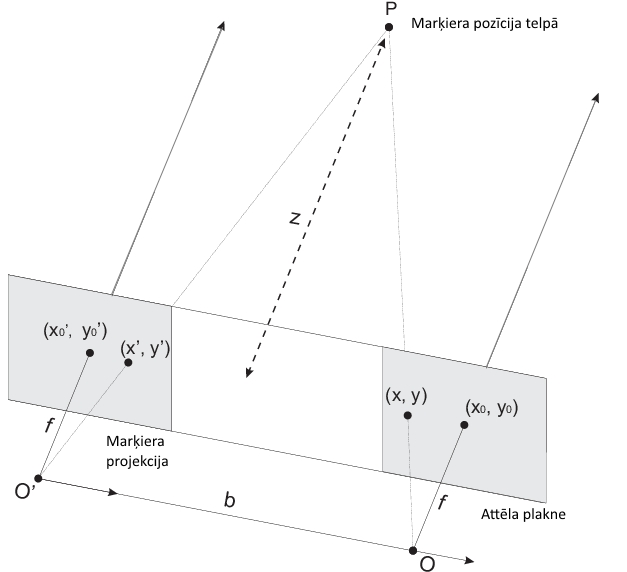
\includegraphics[width=0.8\columnwidth]{images/stereo_1.png}
\begin{center}
\footnotesize{
\textit{\thecimages. attēls. Marķieru pozīciju atrašana 3 dimensiju telpā, izmantojot stereo attēlu projekcijas.}}
\end{center}
\end{center}
\end{samepage}

Uzdevums ir aprēķināt marķiera koordinātes telpā $P_c = (x_c, y_c, z_c)$.
Lai aprēķinātu attālumu līdz marķierim $z_c$, tiek izmantota starpības vērtība $d$ (\textit{disparity}) \cite{AndersonA.S.Souza2012}.

\begin{equation}
d = x' - x
\end{equation}

\begin{equation}
z_c = f \cdot \frac{b}{d}
\end{equation}

\begin{equation}
x_c = z_c \cdot \frac{(x - x_0) + (x' - x_0')}{2 \cdot f}
\end{equation}

\begin{equation}
y_c = z_c \cdot \frac{(y - y_0) + (y' - y_0')}{2 \cdot f}
\end{equation}

Kad ir zināma $P_c$ pozīcija attiecībā pret kameru, lai noteiktu marķiera pozīciju telpā,
nepieciešams izmantot no Oculus Rift iegūto kameras rotācijas matricu $R$ un translācijas vektoru $T$.

\begin{equation}
P_w = R^T \cdot P_c + T
\end{equation}


\refstepcounter{cimages}\label{cimages:online_sample.png}
\vspace{10pt}
\begin{samepage}
\begin{center}
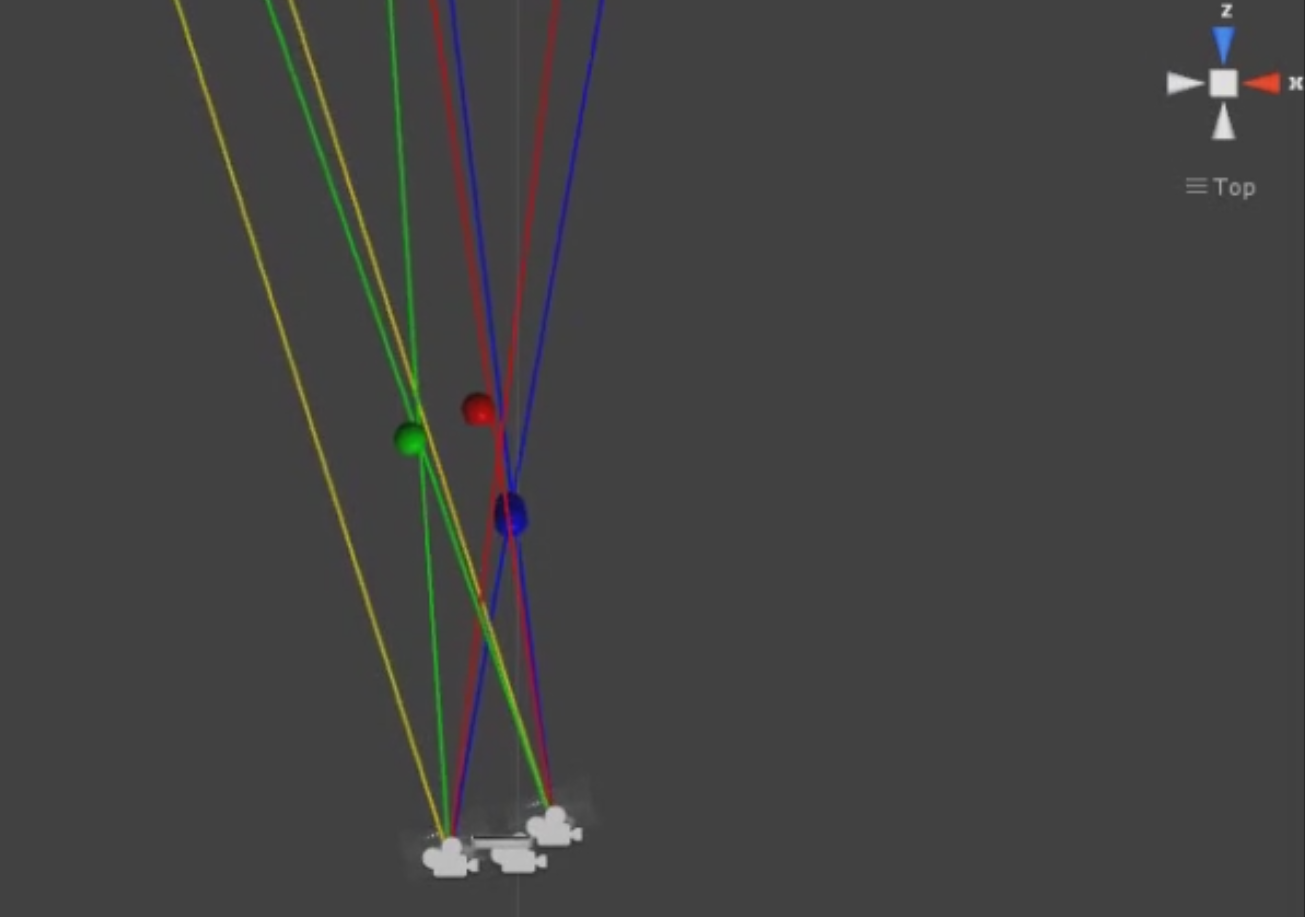
\includegraphics[width=0.5\columnwidth]{images/online_sample.png}
\begin{center}
\footnotesize{
\textit{\thecimages. attēls. Piemērs no Unity 5 dziņa marķieru pozīciju atrašanai telpā. Attēla apakšējā daļā attēlotas Leap Motion kameru pozīcijas.}}
\end{center}
\end{center}
\end{samepage}

\par
Teorētiski, izmantojot infrasarkanās gaismas intensitāti no aktīvajiem marķieriem, kuru uztver 
kamera ar infrasarkanās gaismas filtru, var iegūt objekta pozīciju un orientāciju ar tikai 2 aktīviem marķieriem,
kā to ir demonstrējuši pētnieki no Korejas \cite{ChangHoHan2009}, izmantojot PlayStation 2 kameru.
Šādai sistēmai ir nepieciešamas ātras darbības gaismas diodes, lai varētu ne tikai noteikt
to attālumu, izmantojot intensitātes vērtības, bet arī būtu iespējams pārraidīt datus, ieslēdzot
un izslēdzot tās.

%TODO PnP Solve
% Perspective-n-Point 

\par
Kad ir iegūtas marķieru pozīcijas telpā, un tās identificētas pēc pārraidītā signāla, kas
aprakstīts \ref{section_protocol}. nodaļā, tad ir nepieciešams veikt pozīciju filtrēšanu no
trokšņiem jeb nobīdēm no patiesās pozīcijas. Šādu filtrēšanu ir nepieciešams veikt 2 slāņos.
Vispirms jāfiltrē katra objekta marķiera pozīcijas, lai tām nebūtu novērojama oscilācija,
un pēc tam jāfiltrē arī katrs marķieru kopums, kas apraksta fiziska objekta pozīciju un orientāciju telpā.
Piemēram, galda tenisa raketes ierīcei nepieciešams filtrēt katras diodes pozīciju telpā, tad
pašas raketes pozīciju telpā, kuru nosaka pēc 3 diožu pozīcijām, un visbeidzot raketes orientācijas
filtrāciju, kuru nosaka ar Eilera leņķiem pret plakni, kuru veido 3 diožu pozīcijas.

\par
Kalmana filtra algoritmu \cite{JiangWan1992} diožu pozīcijām telpā var izveidot, izmantojot sekojošus iteratīvus aprēķinus.
Vienādojumos ar \textbf{\textcolor{darkgreen}{zaļu}} krāsu iekrāsoti mainīgie, 
kuru vērtības ir svarīgas tikai algoritma iterācijas ietvaros,
ar \textbf{\textcolor{blue}{zilu}} krāsu iekrāsoti mainīgie, kuri tiek saņemti Kalmana filtra funkcijā, 
ar \textbf{\textcolor{red}{sarkanu}} krāsu iekrāsoti mainīgie, kuri ir rezultāts Kalmana filtra funkcijai, 
bet ar melnu \textbf{krāsu} iekrāsotas konstantes.
\par
Algoritms sastāv no izpildāmiem soļiem:
\begin{enumerate}

\item Prognozēšanas solis. \\
Šajā aprēķinā $x_n$ ir pašreizējās vērtības pozīcijai, jeb vektors $x_n = \{x, y, z\}$. $x_n'$ ir prognozētā
pozīcija, izmantot matemātisko modeli, kas šajā gadījumā balstās uz pārvietojuma ātrumu kopš iepriekšējā kadra
$u_n = \{vx, vy, vz\}$. $x_{n-1}$ ir iepriekšējā iterācijā noteiktā marķiera pozīcija. Sākotnēji
to pieņem kā pirmo mērījumu $z_n$. Savukārt konstante $A$ ir stāvokļa pārvietojuma matrica, kas ir atkarīga
tikai no $x_n$ vērtībām un laika. Marķieru pozīciju filtrācijā tās vērtība ir identitātes matrica,
bet konstante $B$ it kontroles matrica, kura ir atkarīga tikai no laika un $u_n$. Šajā gadījumā $B$ ir
veiktā ceļa aprēķins, zinot pēdējo zināmo pārvietošanās ātrumu un laika starpību
 
\begin{equation}\label{eq:k_1}
\textcolor{darkgreen}{x_{n}'} = A \textcolor{darkgreen}{x_{n-1}}+ B \textcolor{blue}{u_{n}}
\end{equation}

\begin{equation}\label{eq:k_2}
A =  \begin{pmatrix}
1 & 0 & 0\\
0 & 1 & 0\\
0 & 0 & 1
\end{pmatrix}
\end{equation}

\begin{equation}
B = \begin{pmatrix}
\Delta t & 0 & 0\\
0 & \Delta t & 0\\
0 & 0 & \Delta t
\end{pmatrix} 
\end{equation}

Matrica $Q$ ir prognozēšanas soļa kovariance jeb matrica, kas apraksta kļūdas varbūtību \ref{eq:k_1} aprēķinā.
Šīs matricas vērtību var noteikt eksperimentāli, kas šajā implementācijā tika pieņemta 10\% robežās. 

\begin{equation}
\textcolor{darkgreen}{P_{n}'} = A \textcolor{darkgreen}{P_{n-1}} A^T + Q
\end{equation}

\begin{equation}
Q = \begin{pmatrix}
0.1 t & 0 & 0\\
0 & 0.1 t & 0\\
0 & 0 & 0.1 t
\end{pmatrix} 
\end{equation}

\item Novērojumu solis. \\
Šajā solī vienādojumos tiek iekļauta informācija par pašlaik novērotajām marķiera pozīcijām $z_n = \{x, y, z\}$. Ja
marķiera pozīcija īslaicīgi netiek novērota, tad par marķiera pozīciju $x_n$ var pieņemt $x_n'$.
Matrica $H$ apraksta korelāciju starp $x_n$ un $z_n$ jeb cik liela nobīde var būt starp mērījumu un patieso pozīciju,
ja mērījumā nav kļūdas.
Šajā gadījumā situācijā $H$ arī ir identitātes matrica, jo mērījumi bez kļūdām atbilst pozīcijai.

\begin{equation}
\textcolor{darkgreen}{x_n''} = \textcolor{blue}{z_{n}} - H \textcolor{darkgreen}{x_{n}'}
\end{equation}

\begin{equation}
H =  \begin{pmatrix}
1 & 0 & 0\\
0 & 1 & 0\\
0 & 0 & 1
\end{pmatrix}
\end{equation}

Matrica $R$ ir mērījumu kļūdas matrica, kas tiek iegūta eksperimentāli, kur 25\% gadījumu mērījumi ir kļūdaini. 
Aprēķinātā matrica $S$ ir ir inovācijas kovariance, kura ir iekšējais mainīgais katrā iterācijā.
Savukārt matrica $K$ ir Kalmana pieauguma matrica, kura arī ir iekšējais mainīgais katrā iterācijā.

\begin{equation}
\textcolor{darkgreen}{S} = H \textcolor{darkgreen}{P_{n}'} H^T + R
\end{equation}

\begin{equation}
R = \begin{pmatrix}
0.25 t & 0 & 0\\
0 & 0.25 t & 0\\
0 & 0 & 0.25 t
\end{pmatrix} 
\end{equation}

\begin{equation}
\textcolor{darkgreen}{K} = \textcolor{darkgreen}{P_{n}'} H^T S^{-1}
\end{equation}

\item Atjaunināšanas solis. \\
Visbeidzot tiek aprēķināta filtrēta marķiera pozīcija $x_n$ un kovariances matrica.
Abas šīs vērtības tiek nodotas līdz ar jauno mērījumu $z_{n+1}$ nākamajā iterācijā un filtrēšana
atsākas no pirmā soļa. Vienādojumos zemāk $I$ ir identitātes matrica.

\begin{equation}
I =  \begin{pmatrix}
1 & 0 & 0\\
0 & 1 & 0\\
0 & 0 & 1
\end{pmatrix}
\end{equation}

\begin{equation}
\textcolor{red}{x_n} = \textcolor{darkgreen}{x_{n}'} + \textcolor{darkgreen}{K x_{n}''}
\end{equation}

\begin{equation}
\textcolor{red}{P_n} = (I + \textcolor{darkgreen}{K} H) \textcolor{darkgreen}{P_{n}'}
\end{equation}

\end{enumerate}

\refstepcounter{cimages}\label{cimages:kalman_example}
\vspace{10pt}
\begin{samepage}
\begin{center}
\includegraphics[width=0.6\columnwidth]{images/kalman_example.png}
\begin{center}
\footnotesize{
\textit{\thecimages. attēls. Kalmana filtra pielietojuma piemērs marķiera izsekošanai 2D telpā.}}
\end{center}
\end{center}
\end{samepage}

\par 
Izmantojot marķieru pozīciju un orientācijas filtrāciju, tiek iegūta augstāka precizitāte un
stabilitāte sistēmas lietotājam, pārvietojot galvu vai priekšmetu, pie kura piestiprināti marķieri.
Tā kā marķieru pozīcijas tiek klasificētas pēc marķiera sūtītā signāla, kurš nereti ir satur kļūdas,
tad ir nepieciešams projicēt punktus kameras attēla plaknē un pārbaudīt to identifikāciju paralēli 
to pārvietojuma aprēķinam. Šādā veidā ir iespējams iegūt pārraidītos datus pat tad, ja marķieris tiek pārvietots
starp kadriem. Alternatīvi Kalmana filtra algoritmam, ir iespējams pielietot Monte Carlo daļiņu filtru
vai citu filtrēšanas metodi ar prognozēšanas funkcijām.

%%%%%%%%%%%%%%%%%%%%%%%%%%%%%%%%%%%%%%%%%%%%%%%%%%%%%%%%%%%%%%%%%%%%%%%%%%%%%%%%%%%%%%%%%%%%%%%%%%%%%%%%%%%%%%

\newpage
\section{Marķieru sistēmas novērtējums}

\par
Šajā darbā izveidotā cilvēka acij neredzamo marķieru sistēma ir spējīga iegūt objektu pozīcijas un
to orientācijas reālā laikā ar aptuveni 290 ms laika intervālu no brīža, kad nav pieejama informācija
par nekādām marķieru pozīcijām telpā. 
Iegūstot sākotnējās marķieru pozīcijas, to pārvietojuma izmaiņas
var iegūt ātrāk, ņemot vērā, ka no Oculus Rift ir iespējams iegūt kameras odometrijas datus, un 37 Hz
datu pārraides frekvence nodrošina, ka pie ne pārāk straujiem pārvietojumiem ir iespējams izsekot marķieru
pozīcijām un prognozēt to pārvietojumu no kameras iegūtajiem attēliem. Tāpat arī Kalmana filtra implementācija,
kura aprakstīta \ref{section_stereo}.nodaļā, nodrošina sākotnēji iegūtā marķiera pozīcijas nepazaudēšanu.

\par
Sistēmas implementācijā izmantotie algoritmi tika izvēlēti atbilstoši, taču darba izstrādes laikā
atklājās, ka signālu apstrādes algoritmu nozīme ir daudz mazāka kā sākotnēji tika plānots, jo
marķieriem tiešā redzamības zonā nav citu trokšņu kā vien attēla īslaicīga graudainība mainoties apgaismojumam
ar kuru veiksmīgi tiek galā attēla apstrādes algoritmi.

\par
Infrasarkanie aktīvie marķieri jeb infrasarkanās gaismas diodes spēj veiksmīgi pārraidīt datus, kurus
var nolasīt ar Leap Motion infrasarkano kameru. Datu pārraides stabilitāti pie dažādām intensitātēm 
nodrošina attēla apstrādes filtri, taču tā kā 
Leap Motion katram pikselim gaismas intensitāti apraksta baita vērtība (0-255), tad smalkāka gradācija
par to nav pieejama, kas arī pasliktina datu kvalitāti.
Neskatoties uz to, sistēma strādā ļoti stabili, un galvenais veiktspēju ierobežojošais faktors ir kameras
frekvence. No grafika \prettyref{cimages:merijumi_garums_bitos.png}. attēlā var redzēt, ka marķiera identifikatora
garumam ir tieša korelācija ar saņemtā mērījuma laiku no brīža, kad nav informācijas par marķieru pozīcijām līdz brīdim, kad
tas ir ticis atrasts. Saņemtais mērījums ienāk aptuveni pēc 2 reizes ilgāka laika kā ziņojuma pārraides laiks,
jo pārraides sākuma brīdis nav zināms kamerai, kura vēro scēnu. Sinhronizācija notiek tikai pēc pirmā
identifikatora iegūšanas, un marķieris var tikt sākts lasīt, kad tas ir pārraidījis jau pusi datu, ja nav
atrasts datu pārraides sākums. Ar šo sistēmu, izmantošanas laikā, vidēji marķieru atpazīšana notiks 2 reizes
ilgākā laikā kā marķiera pārraides laiks.

\refstepcounter{cimages}\label{cimages:merijumi_garums_bitos.png}
\vspace{10pt}
\begin{samepage}
\begin{center}
\includegraphics[width=0.7\columnwidth]{images/merijumi_garums_bitos.png}
\begin{center}
\footnotesize{
\textit{\thecimages. attēls. Infrasarkano marķieru veiktspēja atkarība no marķiera identifikatora garuma bitos.}}
\end{center}
\end{center}
\end{samepage}

% xzimg

Lai salīdzinātu sistēmas veiktspēju ar tradicionālām redzamo marķieru sistēmām, tika izmantota komerciāla
marķieru bibliotēka XZImg, kura spējīga reālā laikā atrast marķieru pozīcijas un orientācijas dažādos apgaismojumos.
Tā izmanto cilvēka acij redzamus kvadrātveida divkrāsainus jeb bihromatiskus marķierus. 

\refstepcounter{cimages}\label{cimages:merijumi_distance.png}
\vspace{10pt}
\begin{samepage}
\begin{center}
\includegraphics[width=0.7\columnwidth]{images/merijumi_distance.png}
\begin{center}
\footnotesize{
\textit{\thecimages. attēls. Marķieru sistēmu salīdzinājums pēc to darbības attāluma.}}
\end{center}
\end{center}
\end{samepage}

Salīdzinot marķieru sistēmas, tika noskaidrots, ka kvadrātveida redzamās gaismas marķieru sistēma, izmantojot Leap Motion
kamerai līdzvērtīgu 320 x 240 rezolūciju un 11 x 11 cm izmēra drukātu marķieri, darbojas 2 reizes lielākā attālumā,
taču jāņem vērā, ka infrasarkanās gaismas diodes ir neliela izmēra un Leap Motion kameru \\ 640 x 240 rezolūcija arī nav liela. 
Lai iegūtu lielāku darbības attālumu, būtu nepieciešama augstākas izšķirtspējas infrasarkanā kamera.
Vēl interesanti novērot, ka mērījumu laiks ir neatkarīgs no attāluma, un to ietekmē tikai kameras rezolūcija.
Atšķirībā no bezvadu komunikācijas, izmantojot radioviļņus, troksni ir iespējams pilnībā nofiltrēt un attālums
neietekmē signāla kvalitāti.

\refstepcounter{cimages}\label{cimages:xzimg.png}
\vspace{10pt}
\begin{samepage}
\begin{center}
\includegraphics[width=0.4\columnwidth]{images/xzimg.jpg}
\begin{center}
\footnotesize{
\textit{\thecimages. attēls. XZImg komerciālā kvadrātveida bihromatiskā redzamo marķieru implementācija.}}
\end{center}
\end{center}
\end{samepage}

\newpage
\par
Salīdzinot veiktspēju starp tradicionālo marķieru sistēmu un neredzamo infrasarkano marķieru dažādiem kodējumiem,
tika noskaidrots, ka piedāvātā marķieru sistēma, izmantojot Leap Motion 111 Hz kameru ir vismaz 3 reizes lēnāka
kā statisku marķieru sistēma. Neskatoties uz to, piedāvātā infrasarkano marķieru sistēma ir pielietojama 
reālā laikā, kā to parāda \ref{section_implement}.nodaļā aprakstītā galda tenisa spēles implementācija.
Lai iegūtu līdzvērtīgu marķieru atpazīšanas ātrumu, būtu nepieciešama aptuveni 300 Hz frekvences kamera.
Vēl interesanti novērot, ka Mančestras un pāru bitu kodējuma slāņi neuzlabo sistēmas ātrdarbību.
Noteicošais faktors ir tikai pārraidāmā marķiera identifikatora garums bitos. Atkļūdošana nav nepieciešama,
ja vidē nav kameru traucējoši faktori kā, piemēram, sniegs, migla vai putekļi. Iekštelpās kameras attēla troksni pilnībā
likvidē \ref{section_imaging}.nodaļā aprakstītie algoritmi, tāpēc, lai uzlabotu sistēmas ātrdarbību vidē, kurā
nav daudz traucēkļu, kuri aizsedz marķieri, ieteicams neizmantot papildus signāla kodēšanas slāņus, kuri
samazina sistēmas veiktspēju, jo tiem nepieciešams lielāks pārraidāmo bitu apjoms. Neskatoties uz to, ir 
ieteicams izmantot FEC kodēšanu, jo Leap Motion kameras frekvence nav stabila un īslaicīgu kadru iztrūkumu gadījumā
šis kodējums efektīvi palīdz novērst kļūdas.

\refstepcounter{cimages}\label{cimages:merijumi_comparison.png}
\vspace{10pt}
\begin{samepage}
\begin{center}
\includegraphics[width=0.8\columnwidth]{images/merijumi_comparison.png}
\begin{center}
\footnotesize{
\textit{\thecimages. attēls. Infrasarkano marķieru sistēmas slāņu veiktspējas salīdzinājums ar kvadrātveida bihromatiskā marķiera veiktspēju.}}
\end{center}
\end{center}
\end{samepage}

\newpage
\par 
Pētījuma ietvaros tika veikti testi, salīdzinot signāla atkļūdošanas algoritmu darbību dažādās
vidēs. Gadījumā, ja marķiera attēlu aizsedza ūdens tvaiks, tā pārraides ātrums nemainījās, izmantojot
pāru bitu atkļūdošanu. Kā var redzēt \prettyref{cimages:merijumi_parity_tvaikaa_error.png}. attēla grafikā,
tad ūdens tvaiks ietekmēja saņemto datu kvalitāti, un pāru bitu algoritmam nācās labot datus 5 reizes biežāk nekā
vidē bez ūdens tvaikiem. Šādās infrasarkano marķieru sistēmās, ja ir pieejamas kameras ar augstāku frekvenci, būtu ieteicams
implementēt visus atkļūdošanas slāņus, lai nodrošinātu sistēmas stabilitāti jebkādos vides apstākļos.

\refstepcounter{cimages}\label{cimages:vapour.png}
\vspace{10pt}
\begin{samepage}
\begin{center}
\includegraphics[width=0.7\columnwidth]{images/vapour.png}
\begin{center}
\footnotesize{
\textit{\thecimages. attēls. Marķieru sistēmas testēšana, turot Leap Motion sensoru virs verdoša ūdens katla.}}
\end{center}
\end{center}
\end{samepage}


\newpage

\par
Pārraidot papildu informāciju no objekta, pie kura piestiprināti marķieri, kā, piemēram, lietotāja saņemtās komandas 
vai sensoru mērījumus, tā ir jāpārraida, izmantojot Mančestras kodējumu vai arī jāizveido datu apstrādes slānis,
kas nodrošinātu, ka pārraidāmie dati netiktu sajaukti ar pārtraukuma signālu, kas aprakstīts \ref{section_protocol}.nodaļā.

\refstepcounter{cimages}\label{cimages:merijumi_parity_tvaikaa.png}
\vspace{10pt}
\begin{samepage}
\begin{center}
\includegraphics[width=0.8\columnwidth]{images/merijumi_parity_tvaikaa.png}
\begin{center}
\footnotesize{
\textit{\thecimages. attēls. SEC (pāra bitu) atkļūdošanas pārraides ātrums gaisā un ūdens tvaikā.}}
\end{center}
\end{center}
\end{samepage}

\refstepcounter{cimages}\label{cimages:merijumi_parity_tvaikaa_error.png}
\vspace{10pt}
\begin{samepage}
\begin{center}
\includegraphics[width=0.8\columnwidth]{images/merijumi_parity_tvaikaa_error.png}
\begin{center}
\footnotesize{
\textit{\thecimages. attēls. SEC (pāra bitu) atkļūdošanas veiktspēja gaisā un ūdens tvaikā.}}
\end{center}
\end{center}
\end{samepage}



%%%%%%%%%%%%%%%%%%%%%%%%%%%%%%%%%%%%%%%%%%%%%%%%%%%%%%%%%%%%%%%%%%%%%%%%%%%%%%%%%%%%%%%%%%%%%%%%%%%%%%%%%%%%%%

\newpage
\section{Turpmākie pētījumi}\label{section_futher}

\par
Pētījumā tika izveidota infrasarkano marķieru sistēma, izmantojot pašlaik komerciāli brīvi
pieejamas datorsistēmu ierīces. Iegūtās sistēmas vājā vieta ir šo sistēmu piedāvātajās
iespējās un veiktspējā. Piemēram, Leap Motion stereo kamerai ir tikai 111 Hz attēla frekvence,
kura regulāri kadrus filmē ar nobīdēm laikā, kuru dēļ nav iespējams paļauties uz tās 
attēlu frekvenci. Tāpat šai kamerai rezolūcija ir tikai 640 x 240 pikseļi un tās optika
nav piemērota nelielu punktu izšķiršanai lielā attālumā. Kameru savstarpējais attālums arī
neatbilst cilvēka acu attālumam, un galvenais Leap Motion kameru trūkums ir redzamās gaismas
attēla neesamība. Drīzumā tirgū būs pieejamas šādas kameras arī ar redzamās gaismas attēlu,
tāpēc būtu nepieciešams turpināt pētījumus ar jaunākām ierīcēm un izveidot programmas,
kur sistēmas lietotājs nemaz nemana infrasarkano marķieru klātesamību.
\par
Alternatīvi infrasarkano marķieru signālus, iespējams, varētu nolasīt, izmantojot arī 
citu veidu kameras, kā, piemēram, Microsoft Kinect, un šo marķieru pozīcijas izrēķināt
ar Solve PnP algoritmu palīdzību. Šādas implementācijas arī būtu nepieciešams atsevišķi
pētīt un analizēt to veiktspēju.
\par
Šajā darbā maz tika pētīti izveidotās infrasarkano marķieru sistēmas blakusprodukti, kā, 
piemēram, iespēja pārraidīt lietotāja ievades signālus un citus sensoru datus,
izmantojot tos pašus marķierus, kuri ir paredzēti pozīciju noteikšanai. Būtu nepieciešams
veikt papildus pētījumus šādu funkciju veiktspējai.
\par
Vēl būtu nepieciešams veikt pētījumus ar dažādām diožu konfigurācijām, izmēriem un veidiem.
Iespējams, gaismas izkliedējoši ietvari ap diodēm varētu palielināt marķieru atpazīšanas
attālumu.

%%%%%%%%%%%%%%%%%%%%%%%%%%%%%%%%%%%%%%%%%%%%%%%%%%%%%%%%%%%%%%%%%%%%%%%%%%%%%%%%%%%%%%%%%%%%%%%%%%%%%%%%%%%%%%


\newpage
\section{Secinājumi}\label{secinajumi}

\par
Maģistra darba mērķis bija izveidot datorsistēmu, kura nodrošina, ka tās lietotājs
var manipulēt ar fiziskiem objektiem virtuālajā un paplašinātajā realitātē,
izmantojot \\ infrasarkano marķieru sistēmu. Darbā tika aplūkotas jau esošās metodes un
pētījumi redzamo un neredzamo marķieru sistēmām. Tika arī aplūkotas virtuālās
un paplašinātās realitātes attēlošanas iespējas un izvēlēta platforma piedāvātās
sistēmas implementācijai. Pētījuma ietvaros veiksmīgi tika izveidota praktiski izmantojama
sistēma infrasarkano marķieru pozīciju noteikšanai, izmantojot infrasarkanās gaismas
diodes. Iegūtā sistēma ir spējīga darboties reālā laikā, ko pierāda galda tenisa 
sistēmas implementācija, kur objekta pozīcijas un orientācija strauji mainās atkarībā
no raketes novietojuma.
\par
Sistēmas darbību galvenokārt ietekmē Leap Motion infrasarkanās kameras kadru \\ iegūšanas ātrums
un konsistence. Ar pašreizējo Leap Motion kameras versiju ir iespējams iegūt sistēmu, kuras
veiktspēja ir 2 reizes sliktāka nekā tradicionālo marķieru sistēmām, taču jāņem vērā, ka
aktīvajai infrasarkano marķieru sistēmai ir citas priekšrocības, kuras nav iespējamas
tradicionālo marķieru sistēmām. Aktīvo infrasarkano marķieru sistēmu ir iespējams apslēpt
zem fizisku objektu virsmas, kā to pierādīja Begemota rotaļlietas programmas implementācija.
Pie tam fiziskā objekta virsmai var būt nenoteiktas formas. Tāpat ar piedāvāto marķieru
sistēmu ir iespējams pārraidīt papildus datus kā, piemēram, lietotāja darbību signālus
vai sensoru mērījumu datus.
\par
Piedāvātā marķieru sistēma efektīvi darbojas līdz 1.5 m attālumam. Lai iegūtu lielāku
darbības rādiusu, ir nepieciešama augstākas izšķirtspējas kamera un labāka optiskā sistēma.
Kameras iegūtajos attēlos visus trokšņus vairumā gadījumu ir iespējams attīrīt, izmantojot
attēlu apstrādes algoritmus. Bet, ja sistēmu ir paredzēts izmantot vidēs, kur gaisā starp
kameru un marķieri var būt traucēkļi kā, piemēram, sniegs vai migla, tad signālu apstrādes
kļūdu labošanas algoritmi veiksmīgi var uzlabot signāla kvalitāti, neskatoties uz attēlā
esošajiem trokšņiem. 
\par
Iegūtās objektu pozīcijas un orientācijas sakrīt ar reālā vidē esošo objektu pozīcijām.
To parāda izveidotajās programmās fizisko objektu 3D repliku pārklājumu sakritība ar 
no Leap Motion stereo kamerām iegūto fona attēlu, kurā ir redzami šie fiziskie objekti.
Neskatoties uz to, ka attālums starp Leap Motion kamerām nesakrīt ar attālumu starp cilvēka
acīm, iegūtā paplašinātās realitātes ilūzija, kura tiek projicēta acu priekšā, izmantojot
Oculus Rift DK2, ir ar pietiekami augstu ticamību, lai tās lietotājs varētu komfortabli izmantot
šajā pētījumā izveidotās programmas.
\par
Visi sistēmas izveidošanai nepieciešamie datorsistēmu un programmatūras komponenti ir brīvi
pieejami tirgū, un to var pielietot ļoti dažādiem mērķiem. Galvenais pielietojums, kas tika
notestēts ar izveidotajām programmām, ir paplašinātās realitātes nodrošināšanā, lai programmatūra
varētu noteikt fizisku objektu atrašanās vietas. Diemžēl no šobrīd pieejamās Leap Motion
stereo kameras ir iespējams iegūt tikai augstas frekvences \\ infrasarkano attēlu, taču
tuvākajā laikā tirgū būs pieejami jaunāku versiju kameru modeļi, no kuriem būs iegūstams
arī redzamās gaismas attēls. Izmantojot šādas iekārtas, būs iespējams pilnībā noslēpt
marķieru klātbūtni no sistēmas lietotāja redzamā attēla. 
\par
Vēl praktiski pielietojumi izveidotajai sistēmai būtu robotikā neregulāru priekšmetu pozīciju un
orientāciju precīzākai noteikšanai. Atšķirībā no citām šajā pētījumā apskatītājam attēlu apstrādes metodēm, šajā 
pētījumā piedāvātā marķieru sistēma iegūst viennozīmīgas marķieru pozīcijas, kuras
nevar sajaukt ar citiem punktiem dinamiskā vidē.


%%%%%%%%%%%%%%%%%%%%%%%%%%%%%%%%%%%%%%%%%%%%%%%%%%%%%%%%%%%%%%%%%%%%%%%%%%%%%%%%%%%%%%%%%%%%%%%%%%%%%%%%%%%%%%

\newpage
\section{Terminu vārdnīca}\label{section_futher}

\begin{itemize}

% Aa, Āā, Bb, Cc, Čč, Dd, Ee, Ēē, Ff, Gg, Ģģ, Hh, Ii, Īī, Jj, Kk, Ķķ, Ll, Ļļ, Mm, Nn, Ņņ, Oo, Pp, Rr, Ss, Šš, Tt, Uu, Ūū, Vv, Zz, Žž.

\item \textbf{Aktīvais marķieris} - marķieris, kas var dinamiski mainīt pārraidāmos identifikācijas datus laikā bez ārējām fiziskām manipulācijām.

\item \textbf{Haptiskā atgriezeniskā saite} – taustes sajūtu izraisošs datorsistēmas interfeiss.

\item \textbf{DEC (Double bit Error Correction) – divu bitu automātiska atkļūdošana} – 
Algoritms, kas paredzēts datu signāla virknes 2 kļūdainu bitu atkļūdošanai bez papildus pieprasījumiem.

\item \textbf{EKF-SLAM (Extended Kalman Filter - Simultaneous Localization And Mapping)} - algoritms, kas veic kartēšanu un pašlokalizāciju iepriekš nezināmās vidēs, izmantojot paplašināto Kalmana filtru.

\item \textbf{HMD (Head Mounted Display) – pie galvas piestiprināts ekrāns } – iekārta, kura tiek piestiprināta pie galvas, aizklājot visu vai daļu no redzes lauka, kurā tiek katrai acij projicēts savs virtuāls attēls.

\item \textbf{FEC (Forward Error Correction) – uz priekšu ejoša automātiska atkļūdošana} – 
Datu signāla atkļūdošanas algoritms, izmantojot papildus signāla dublikātu kadrus

\item \textbf{FOV (Field of View) – redzes lauks} – redzes lauks no acij pa abscisu vai ordinātu asi, parasti tiek mērīts ar leņķi grādos

\item \textbf{Infrasarkanā gaisma} – gaisma neredzamās gaismas spektrā ar viļņa garumu no 700 nm līdz 1 mm.

\item \textbf{Li-Fi (Light Fidelity)} – datu apmaiņas sistēma, izmantojot redzamās vai neredzamās gaismas raidītājus un uztvērējus.

\item \textbf{Marķieris} - punkts telpā, kas pievienots objekta, un palīdz noteikt tā pozīciju. Vairāki marķieri kopā palīdz noteikt arī šī objekta orientāciju telpā. 

\item \textbf{Monochromatic markers – monohromatiskie marķieri - divkrāsaini marķieri} – parasti melni kvadrātveida
marķieri, kas nodrukāti uz baltas lapas.

\item \textbf{Odometrija} - sensoru dati par objekta pārvietojumu un orientāciju laikā.

\item \textbf{Paplašinātā realitāte - Augmented reality} - Datorā veidota mākslīga 3D vide, kura tiek attēlota pāri cilvēkam redzamajai videi, saglabājot redzamu arī apkārtējo dabīgo vidi. 

\item \textbf{Pasīvais marķieris} - marķieris, kas var nevar mainīt savu identifikācijas informāciju laikā bez ārējām fiziskām manipulācijām.

\item \textbf{Pavediens - thread} - paralēls izpildāmais process programmatūrā.

\item \textbf{SEC (Single bit Error Correction) – viena bitu automātiska atkļūdošana} – 
Algoritms, kas paredzēts datu signāla virknes viena kļūdaina bita atkļūdošanai bez papildus pieprasījumiem.

\item \textbf{Solve PnP (Solve Perspective-n-Point problem) - Perspektīvas un punkta problēmas algoritms} – Algoritms, kas
paredzēts, lai no viena 2D attēla iegūtu izdalītu un iepriekš zināmu ģeometrisku punktu konfigurāciju pozīciju un orientāciju
3D telpā. Standarta risinājumos ir nepieciešama vismaz 3 punktu konfigurācija.

\item \textbf{Stereo kamera} - divas kameras, kuras pozicionētas vienā virzienā un atrodas vienā plaknē ar noteiktu attālumu.

\item \textbf{VR (Virtuālā realitāte) - Virtual reality} - Datorā veidota mākslīga trīsdimensiju vide, kas rada realitātes ilūziju.

\item \textbf{VRD (Virtual Retina Display) - Virtuālais tīklenes ekrāns} - sistēma, kas attēlu projicē tieši uz acs tīklenes, neizmantojot acij priekšā stāvošufield ov ekrānu tehnoloģiju.

\item \textbf{XOR} - izslēdzošais "vai" operators bitu aritmētikā.

\end{itemize}

%%%%%%%%%%%%%%%%%%%%%%%%%%%%%%%%%%%%%%%%%%%%%%%%%%%%%%%%%%%%%%%%%%%%%%%%%%%%%%%%%%%%%%%%%%%%%%%%%%%%%%%%%%%%%%



\newpage
\nocite{*} % include all bibliography
\addcontentsline{toc}{section}{8. Izmantotā literatūra}
\renewcommand{\refname}{8. Izmantotā literatūra}
\bibliographystyle{deplain}
\bibliography{bibliography}


\end{document}